\NeedsTeXFormat{LaTeX2e}
%\documentstyle[makeidx]{cmmp}
\documentclass[11pt,a4paper]{book}

\usepackage{makeidx}
% \usepackage{astron}
\usepackage{psfig}
\newcommand{\psdir}{/export/home/starck/Main/sadam/tex/report/FIG}
\psfigurepath{\psdir/mr1:\psdir/demo:\psdir/cours:\psdir/edge:\psdir/compress:\psdir/fractal:\psdir/detect:\psdir/book98:\psdir/entropy:\psdir/iso:\psdir/cours}


\def\aa{{A\&A } }
\def\aj{{AJ} }
\def\apj{{ApJ\ }}
\def\va{{ Vistas in Astronomy}}
\def\pasp{{ PASP\ }}
 
\def\projmw{MR/2 }
\def\defprojmw{Multiscale Entropy and Applications}

% \makeindex
%% Psfig/TeX 
\def\PsfigVersion{1.9}
% dvips version
%
% All psfig/tex software, documentation, and related files
% in this distribution of psfig/tex are 
% Copyright 1987, 1988, 1991 Trevor J. Darrell
%
% Permission is granted for use and non-profit distribution of psfig/tex 
% providing that this notice is clearly maintained. The right to
% distribute any portion of psfig/tex for profit or as part of any commercial
% product is specifically reserved for the author(s) of that portion.
%
% *** Feel free to make local modifications of psfig as you wish,
% *** but DO NOT post any changed or modified versions of ``psfig''
% *** directly to the net. Send them to me and I'll try to incorporate
% *** them into future versions. If you want to take the psfig code 
% *** and make a new program (subject to the copyright above), distribute it, 
% *** (and maintain it) that's fine, just don't call it psfig.
%
% Bugs and improvements to trevor@media.mit.edu.
%
% Thanks to Greg Hager (GDH) and Ned Batchelder for their contributions
% to the original version of this project.
%
% Modified by J. Daniel Smith on 9 October 1990 to accept the
% %%BoundingBox: comment with or without a space after the colon.  Stole
% file reading code from Tom Rokicki's EPSF.TEX file (see below).
%
% More modifications by J. Daniel Smith on 29 March 1991 to allow the
% the included PostScript figure to be rotated.  The amount of
% rotation is specified by the "angle=" parameter of the \psfig command.
%
% Modified by Robert Russell on June 25, 1991 to allow users to specify
% .ps filenames which don't yet exist, provided they explicitly provide
% boundingbox information via the \psfig command. Note: This will only work
% if the "file=" parameter follows all four "bb???=" parameters in the
% command. This is due to the order in which psfig interprets these params.
%
%  3 Jul 1991	JDS	check if file already read in once
%  4 Sep 1991	JDS	fixed incorrect computation of rotated
%			bounding box
% 25 Sep 1991	GVR	expanded synopsis of \psfig
% 14 Oct 1991	JDS	\fbox code from LaTeX so \psdraft works with TeX
%			changed \typeout to \ps@typeout
% 17 Oct 1991	JDS	added \psscalefirst and \psrotatefirst
%

% From: gvr@cs.brown.edu (George V. Reilly)
%
% \psdraft	draws an outline box, but doesn't include the figure
%		in the DVI file.  Useful for previewing.
%
% \psfull	includes the figure in the DVI file (default).
%
% \psscalefirst width= or height= specifies the size of the figure
% 		before rotation.
% \psrotatefirst (default) width= or height= specifies the size of the
% 		 figure after rotation.  Asymetric figures will
% 		 appear to shrink.
%
% \psfigurepath#1	sets the path to search for the figure
%
% \psfig
% usage: \psfig{file=, figure=, height=, width=,
%			bbllx=, bblly=, bburx=, bbury=,
%			rheight=, rwidth=, clip=, angle=, silent=}
%
%	"file" is the filename.  If no path name is specified and the
%		file is not found in the current directory,
%		it will be looked for in directory \psfigurepath.
%	"figure" is a synonym for "file".
%	By default, the width and height of the figure are taken from
%		the BoundingBox of the figure.
%	If "width" is specified, the figure is scaled so that it has
%		the specified width.  Its height changes proportionately.
%	If "height" is specified, the figure is scaled so that it has
%		the specified height.  Its width changes proportionately.
%	If both "width" and "height" are specified, the figure is scaled
%		anamorphically.
%	"bbllx", "bblly", "bburx", and "bbury" control the PostScript
%		BoundingBox.  If these four values are specified
%               *before* the "file" option, the PSFIG will not try to
%               open the PostScript file.
%	"rheight" and "rwidth" are the reserved height and width
%		of the figure, i.e., how big TeX actually thinks
%		the figure is.  They default to "width" and "height".
%	The "clip" option ensures that no portion of the figure will
%		appear outside its BoundingBox.  "clip=" is a switch and
%		takes no value, but the `=' must be present.
%	The "angle" option specifies the angle of rotation (degrees, ccw).
%	The "silent" option makes \psfig work silently.
%

% check to see if macros already loaded in (maybe some other file says
% "\input psfig") ...
\ifx\undefined\psfig\else\endinput\fi

%
% from a suggestion by eijkhout@csrd.uiuc.edu to allow
% loading as a style file. Changed to avoid problems
% with amstex per suggestion by jbence@math.ucla.edu

\let\LaTeXAtSign=\@
\let\@=\relax
\edef\psfigRestoreAt{\catcode`\@=\number\catcode`@\relax}
%\edef\psfigRestoreAt{\catcode`@=\number\catcode`@\relax}
\catcode`\@=11\relax
\newwrite\@unused
\def\ps@typeout#1{{\let\protect\string\immediate\write\@unused{#1}}}
\ps@typeout{psfig/tex \PsfigVersion}

%% Here's how you define your figure path.  Should be set up with null
%% default and a user useable definition.

\def\figurepath{./}
\def\psfigurepath#1{\edef\figurepath{#1}}

%
% @psdo control structure -- similar to Latex @for.
% I redefined these with different names so that psfig can
% be used with TeX as well as LaTeX, and so that it will not 
% be vunerable to future changes in LaTeX's internal
% control structure,
%
\def\@nnil{\@nil}
\def\@empty{}
\def\@psdonoop#1\@@#2#3{}
\def\@psdo#1:=#2\do#3{\edef\@psdotmp{#2}\ifx\@psdotmp\@empty \else
    \expandafter\@psdoloop#2,\@nil,\@nil\@@#1{#3}\fi}
\def\@psdoloop#1,#2,#3\@@#4#5{\def#4{#1}\ifx #4\@nnil \else
       #5\def#4{#2}\ifx #4\@nnil \else#5\@ipsdoloop #3\@@#4{#5}\fi\fi}
\def\@ipsdoloop#1,#2\@@#3#4{\def#3{#1}\ifx #3\@nnil 
       \let\@nextwhile=\@psdonoop \else
      #4\relax\let\@nextwhile=\@ipsdoloop\fi\@nextwhile#2\@@#3{#4}}
\def\@tpsdo#1:=#2\do#3{\xdef\@psdotmp{#2}\ifx\@psdotmp\@empty \else
    \@tpsdoloop#2\@nil\@nil\@@#1{#3}\fi}
\def\@tpsdoloop#1#2\@@#3#4{\def#3{#1}\ifx #3\@nnil 
       \let\@nextwhile=\@psdonoop \else
      #4\relax\let\@nextwhile=\@tpsdoloop\fi\@nextwhile#2\@@#3{#4}}
% 
% \fbox is defined in latex.tex; so if \fbox is undefined, assume that
% we are not in LaTeX.
% Perhaps this could be done better???
\ifx\undefined\fbox
% \fbox code from modified slightly from LaTeX
\newdimen\fboxrule
\newdimen\fboxsep
\newdimen\ps@tempdima
\newbox\ps@tempboxa
\fboxsep = 3pt
\fboxrule = .4pt
\long\def\fbox#1{\leavevmode\setbox\ps@tempboxa\hbox{#1}\ps@tempdima\fboxrule
    \advance\ps@tempdima \fboxsep \advance\ps@tempdima \dp\ps@tempboxa
   \hbox{\lower \ps@tempdima\hbox
  {\vbox{\hrule height \fboxrule
          \hbox{\vrule width \fboxrule \hskip\fboxsep
          \vbox{\vskip\fboxsep \box\ps@tempboxa\vskip\fboxsep}\hskip 
                 \fboxsep\vrule width \fboxrule}
                 \hrule height \fboxrule}}}}
\fi
%
%%%%%%%%%%%%%%%%%%%%%%%%%%%%%%%%%%%%%%%%%%%%%%%%%%%%%%%%%%%%%%%%%%%
% file reading stuff from epsf.tex
%   EPSF.TEX macro file:
%   Written by Tomas Rokicki of Radical Eye Software, 29 Mar 1989.
%   Revised by Don Knuth, 3 Jan 1990.
%   Revised by Tomas Rokicki to accept bounding boxes with no
%      space after the colon, 18 Jul 1990.
%   Portions modified/removed for use in PSFIG package by
%      J. Daniel Smith, 9 October 1990.
%
\newread\ps@stream
\newif\ifnot@eof       % continue looking for the bounding box?
\newif\if@noisy        % report what you're making?
\newif\if@atend        % %%BoundingBox: has (at end) specification
\newif\if@psfile       % does this look like a PostScript file?
%
% PostScript files should start with `%!'
%
{\catcode`\%=12\global\gdef\epsf@start{%!}}
\def\epsf@PS{PS}
%
\def\epsf@getbb#1{%
%
%   The first thing we need to do is to open the
%   PostScript file, if possible.
%
\openin\ps@stream=#1
\ifeof\ps@stream\ps@typeout{Error, File #1 not found}\else
%
%   Okay, we got it. Now we'll scan lines until we find one that doesn't
%   start with %. We're looking for the bounding box comment.
%
   {\not@eoftrue \chardef\other=12
    \def\do##1{\catcode`##1=\other}\dospecials \catcode`\ =10
    \loop
       \if@psfile
	  \read\ps@stream to \epsf@fileline
       \else{
	  \obeyspaces
          \read\ps@stream to \epsf@tmp\global\let\epsf@fileline\epsf@tmp}
       \fi
       \ifeof\ps@stream\not@eoffalse\else
%
%   Check the first line for `%!'.  Issue a warning message if its not
%   there, since the file might not be a PostScript file.
%
       \if@psfile\else
       \expandafter\epsf@test\epsf@fileline:. \\%
       \fi
%
%   We check to see if the first character is a % sign;
%   if so, we look further and stop only if the line begins with
%   `%%BoundingBox:' and the `(atend)' specification was not found.
%   That is, the only way to stop is when the end of file is reached,
%   or a `%%BoundingBox: llx lly urx ury' line is found.
%
          \expandafter\epsf@aux\epsf@fileline:. \\%
       \fi
   \ifnot@eof\repeat
   }\closein\ps@stream\fi}%
%
% This tests if the file we are reading looks like a PostScript file.
%
\long\def\epsf@test#1#2#3:#4\\{\def\epsf@testit{#1#2}
			\ifx\epsf@testit\epsf@start\else
\ps@typeout{Warning! File does not start with `\epsf@start'.  It may not be a PostScript file.}
			\fi
			\@psfiletrue} % don't test after 1st line
%
%   We still need to define the tricky \epsf@aux macro. This requires
%   a couple of magic constants for comparison purposes.
%
{\catcode`\%=12\global\let\epsf@percent=%\global\def\epsf@bblit{%BoundingBox}}
%
%
%   So we're ready to check for `%BoundingBox:' and to grab the
%   values if they are found.  We continue searching if `(at end)'
%   was found after the `%BoundingBox:'.
%
\long\def\epsf@aux#1#2:#3\\{\ifx#1\epsf@percent
   \def\epsf@testit{#2}\ifx\epsf@testit\epsf@bblit
	\@atendfalse
        \epsf@atend #3 . \\%
	\if@atend	
	   \if@verbose{
		\ps@typeout{psfig: found `(atend)'; continuing search}
	   }\fi
        \else
        \epsf@grab #3 . . . \\%
        \not@eoffalse
        \global\no@bbfalse
        \fi
   \fi\fi}%
%
%   Here we grab the values and stuff them in the appropriate definitions.
%
\def\epsf@grab #1 #2 #3 #4 #5\\{%
   \global\def\epsf@llx{#1}\ifx\epsf@llx\empty
      \epsf@grab #2 #3 #4 #5 .\\\else
   \global\def\epsf@lly{#2}%
   \global\def\epsf@urx{#3}\global\def\epsf@ury{#4}\fi}%
%
% Determine if the stuff following the %%BoundingBox is `(atend)'
% J. Daniel Smith.  Copied from \epsf@grab above.
%
\def\epsf@atendlit{(atend)} 
\def\epsf@atend #1 #2 #3\\{%
   \def\epsf@tmp{#1}\ifx\epsf@tmp\empty
      \epsf@atend #2 #3 .\\\else
   \ifx\epsf@tmp\epsf@atendlit\@atendtrue\fi\fi}


% End of file reading stuff from epsf.tex
%%%%%%%%%%%%%%%%%%%%%%%%%%%%%%%%%%%%%%%%%%%%%%%%%%%%%%%%%%%%%%%%%%%

%%%%%%%%%%%%%%%%%%%%%%%%%%%%%%%%%%%%%%%%%%%%%%%%%%%%%%%%%%%%%%%%%%%
% trigonometry stuff from "trig.tex"
\chardef\psletter = 11 % won't conflict with \begin{letter} now...
\chardef\other = 12

\newif \ifdebug %%% turn me on to see TeX hard at work ...
\newif\ifc@mpute %%% don't need to compute some values
\c@mputetrue % but assume that we do

\let\then = \relax
\def\r@dian{pt }
\let\r@dians = \r@dian
\let\dimensionless@nit = \r@dian
\let\dimensionless@nits = \dimensionless@nit
\def\internal@nit{sp }
\let\internal@nits = \internal@nit
\newif\ifstillc@nverging
\def \Mess@ge #1{\ifdebug \then \message {#1} \fi}

{ %%% Things that need abnormal catcodes %%%
	\catcode `\@ = \psletter
	\gdef \nodimen {\expandafter \n@dimen \the \dimen}
	\gdef \term #1 #2 #3%
	       {\edef \t@ {\the #1}%%% freeze parameter 1 (count, by value)
		\edef \t@@ {\expandafter \n@dimen \the #2\r@dian}%
				   %%% freeze parameter 2 (dimen, by value)
		\t@rm {\t@} {\t@@} {#3}%
	       }
	\gdef \t@rm #1 #2 #3%
	       {{%
		\count 0 = 0
		\dimen 0 = 1 \dimensionless@nit
		\dimen 2 = #2\relax
		\Mess@ge {Calculating term #1 of \nodimen 2}%
		\loop
		\ifnum	\count 0 < #1
		\then	\advance \count 0 by 1
			\Mess@ge {Iteration \the \count 0 \space}%
			\Multiply \dimen 0 by {\dimen 2}%
			\Mess@ge {After multiplication, term = \nodimen 0}%
			\Divide \dimen 0 by {\count 0}%
			\Mess@ge {After division, term = \nodimen 0}%
		\repeat
		\Mess@ge {Final value for term #1 of 
				\nodimen 2 \space is \nodimen 0}%
		\xdef \Term {#3 = \nodimen 0 \r@dians}%
		\aftergroup \Term
	       }}
	\catcode `\p = \other
	\catcode `\t = \other
	\gdef \n@dimen #1pt{#1} %%% throw away the ``pt''
}

\def \Divide #1by #2{\divide #1 by #2} %%% just a synonym

\def \Multiply #1by #2%%% allows division of a dimen by a dimen
       {{%%% should really freeze parameter 2 (dimen, passed by value)
	\count 0 = #1\relax
	\count 2 = #2\relax
	\count 4 = 65536
	\Mess@ge {Before scaling, count 0 = \the \count 0 \space and
			count 2 = \the \count 2}%
	\ifnum	\count 0 > 32767 %%% do our best to avoid overflow
	\then	\divide \count 0 by 4
		\divide \count 4 by 4
	\else	\ifnum	\count 0 < -32767
		\then	\divide \count 0 by 4
			\divide \count 4 by 4
		\else
		\fi
	\fi
	\ifnum	\count 2 > 32767 %%% while retaining reasonable accuracy
	\then	\divide \count 2 by 4
		\divide \count 4 by 4
	\else	\ifnum	\count 2 < -32767
		\then	\divide \count 2 by 4
			\divide \count 4 by 4
		\else
		\fi
	\fi
	\multiply \count 0 by \count 2
	\divide \count 0 by \count 4
	\xdef \product {#1 = \the \count 0 \internal@nits}%
	\aftergroup \product
       }}

\def\r@duce{\ifdim\dimen0 > 90\r@dian \then   % sin(x+90) = sin(180-x)
		\multiply\dimen0 by -1
		\advance\dimen0 by 180\r@dian
		\r@duce
	    \else \ifdim\dimen0 < -90\r@dian \then  % sin(-x) = sin(360+x)
		\advance\dimen0 by 360\r@dian
		\r@duce
		\fi
	    \fi}

\def\Sine#1%
       {{%
	\dimen 0 = #1 \r@dian
	\r@duce
	\ifdim\dimen0 = -90\r@dian \then
	   \dimen4 = -1\r@dian
	   \c@mputefalse
	\fi
	\ifdim\dimen0 = 90\r@dian \then
	   \dimen4 = 1\r@dian
	   \c@mputefalse
	\fi
	\ifdim\dimen0 = 0\r@dian \then
	   \dimen4 = 0\r@dian
	   \c@mputefalse
	\fi
%
	\ifc@mpute \then
        	% convert degrees to radians
		\divide\dimen0 by 180
		\dimen0=3.141592654\dimen0
%
		\dimen 2 = 3.1415926535897963\r@dian %%% a well-known constant
		\divide\dimen 2 by 2 %%% we only deal with -pi/2 : pi/2
		\Mess@ge {Sin: calculating Sin of \nodimen 0}%
		\count 0 = 1 %%% see power-series expansion for sine
		\dimen 2 = 1 \r@dian %%% ditto
		\dimen 4 = 0 \r@dian %%% ditto
		\loop
			\ifnum	\dimen 2 = 0 %%% then we've done
			\then	\stillc@nvergingfalse 
			\else	\stillc@nvergingtrue
			\fi
			\ifstillc@nverging %%% then calculate next term
			\then	\term {\count 0} {\dimen 0} {\dimen 2}%
				\advance \count 0 by 2
				\count 2 = \count 0
				\divide \count 2 by 2
				\ifodd	\count 2 %%% signs alternate
				\then	\advance \dimen 4 by \dimen 2
				\else	\advance \dimen 4 by -\dimen 2
				\fi
		\repeat
	\fi		
			\xdef \sine {\nodimen 4}%
       }}

% Now the Cosine can be calculated easily by calling \Sine
\def\Cosine#1{\ifx\sine\UnDefined\edef\Savesine{\relax}\else
		             \edef\Savesine{\sine}\fi
	{\dimen0=#1\r@dian\advance\dimen0 by 90\r@dian
	 \Sine{\nodimen 0}
	 \xdef\cosine{\sine}
	 \xdef\sine{\Savesine}}}	      
% end of trig stuff
%%%%%%%%%%%%%%%%%%%%%%%%%%%%%%%%%%%%%%%%%%%%%%%%%%%%%%%%%%%%%%%%%%%%

\def\psdraft{
	\def\@psdraft{0}
	%\ps@typeout{draft level now is \@psdraft \space . }
}
\def\psfull{
	\def\@psdraft{100}
	%\ps@typeout{draft level now is \@psdraft \space . }
}

\psfull

\newif\if@scalefirst
\def\psscalefirst{\@scalefirsttrue}
\def\psrotatefirst{\@scalefirstfalse}
\psrotatefirst

\newif\if@draftbox
\def\psnodraftbox{
	\@draftboxfalse
}
\def\psdraftbox{
	\@draftboxtrue
}
\@draftboxtrue

\newif\if@prologfile
\newif\if@postlogfile
\def\pssilent{
	\@noisyfalse
}
\def\psnoisy{
	\@noisytrue
}
\psnoisy
%%% These are for the option list.
%%% A specification of the form a = b maps to calling \@p@@sa{b}
\newif\if@bbllx
\newif\if@bblly
\newif\if@bburx
\newif\if@bbury
\newif\if@height
\newif\if@width
\newif\if@rheight
\newif\if@rwidth
\newif\if@angle
\newif\if@clip
\newif\if@verbose
\def\@p@@sclip#1{\@cliptrue}


\newif\if@decmpr

%%% GDH 7/26/87 -- changed so that it first looks in the local directory,
%%% then in a specified global directory for the ps file.
%%% RPR 6/25/91 -- changed so that it defaults to user-supplied name if
%%% boundingbox info is specified, assuming graphic will be created by
%%% print time.
%%% TJD 10/19/91 -- added bbfile vs. file distinction, and @decmpr flag

\def\@p@@sfigure#1{\def\@p@sfile{null}\def\@p@sbbfile{null}
	        \openin1=#1.bb
		\ifeof1\closein1
	        	\openin1=\figurepath#1.bb
			\ifeof1\closein1
			        \openin1=#1
				\ifeof1\closein1%
				       \openin1=\figurepath#1
					\ifeof1
					   \ps@typeout{Error, File #1 not found}
						\if@bbllx\if@bblly
				   		\if@bburx\if@bbury
			      				\def\@p@sfile{#1}%
			      				\def\@p@sbbfile{#1}%
							\@decmprfalse
				  	   	\fi\fi\fi\fi
					\else\closein1
				    		\def\@p@sfile{\figurepath#1}%
				    		\def\@p@sbbfile{\figurepath#1}%
						\@decmprfalse
	                       		\fi%
			 	\else\closein1%
					\def\@p@sfile{#1}
					\def\@p@sbbfile{#1}
					\@decmprfalse
			 	\fi
			\else
				\def\@p@sfile{\figurepath#1}
				\def\@p@sbbfile{\figurepath#1.bb}
				\@decmprtrue
			\fi
		\else
			\def\@p@sfile{#1}
			\def\@p@sbbfile{#1.bb}
			\@decmprtrue
		\fi}

\def\@p@@sfile#1{\@p@@sfigure{#1}}

\def\@p@@sbbllx#1{
		%\ps@typeout{bbllx is #1}
		\@bbllxtrue
		\dimen100=#1
		\edef\@p@sbbllx{\number\dimen100}
}
\def\@p@@sbblly#1{
		%\ps@typeout{bblly is #1}
		\@bbllytrue
		\dimen100=#1
		\edef\@p@sbblly{\number\dimen100}
}
\def\@p@@sbburx#1{
		%\ps@typeout{bburx is #1}
		\@bburxtrue
		\dimen100=#1
		\edef\@p@sbburx{\number\dimen100}
}
\def\@p@@sbbury#1{
		%\ps@typeout{bbury is #1}
		\@bburytrue
		\dimen100=#1
		\edef\@p@sbbury{\number\dimen100}
}
\def\@p@@sheight#1{
		\@heighttrue
		\dimen100=#1
   		\edef\@p@sheight{\number\dimen100}
		%\ps@typeout{Height is \@p@sheight}
}
\def\@p@@swidth#1{
		%\ps@typeout{Width is #1}
		\@widthtrue
		\dimen100=#1
		\edef\@p@swidth{\number\dimen100}
}
\def\@p@@srheight#1{
		%\ps@typeout{Reserved height is #1}
		\@rheighttrue
		\dimen100=#1
		\edef\@p@srheight{\number\dimen100}
}
\def\@p@@srwidth#1{
		%\ps@typeout{Reserved width is #1}
		\@rwidthtrue
		\dimen100=#1
		\edef\@p@srwidth{\number\dimen100}
}
\def\@p@@sangle#1{
		%\ps@typeout{Rotation is #1}
		\@angletrue
%		\dimen100=#1
		\edef\@p@sangle{#1} %\number\dimen100}
}
\def\@p@@ssilent#1{ 
		\@verbosefalse
}
\def\@p@@sprolog#1{\@prologfiletrue\def\@prologfileval{#1}}
\def\@p@@spostlog#1{\@postlogfiletrue\def\@postlogfileval{#1}}
\def\@cs@name#1{\csname #1\endcsname}
\def\@setparms#1=#2,{\@cs@name{@p@@s#1}{#2}}
%
% initialize the defaults (size the size of the figure)
%
\def\ps@init@parms{
		\@bbllxfalse \@bbllyfalse
		\@bburxfalse \@bburyfalse
		\@heightfalse \@widthfalse
		\@rheightfalse \@rwidthfalse
		\def\@p@sbbllx{}\def\@p@sbblly{}
		\def\@p@sbburx{}\def\@p@sbbury{}
		\def\@p@sheight{}\def\@p@swidth{}
		\def\@p@srheight{}\def\@p@srwidth{}
		\def\@p@sangle{0}
		\def\@p@sfile{} \def\@p@sbbfile{}
		\def\@p@scost{10}
		\def\@sc{}
		\@prologfilefalse
		\@postlogfilefalse
		\@clipfalse
		\if@noisy
			\@verbosetrue
		\else
			\@verbosefalse
		\fi
}
%
% Go through the options setting things up.
%
\def\parse@ps@parms#1{
	 	\@psdo\@psfiga:=#1\do
		   {\expandafter\@setparms\@psfiga,}}
%
% Compute bb height and width
%
\newif\ifno@bb
\def\bb@missing{
	\if@verbose{
		\ps@typeout{psfig: searching \@p@sbbfile \space  for bounding box}
	}\fi
	\no@bbtrue
	\epsf@getbb{\@p@sbbfile}
        \ifno@bb \else \bb@cull\epsf@llx\epsf@lly\epsf@urx\epsf@ury\fi
}	
\def\bb@cull#1#2#3#4{
	\dimen100=#1 bp\edef\@p@sbbllx{\number\dimen100}
	\dimen100=#2 bp\edef\@p@sbblly{\number\dimen100}
	\dimen100=#3 bp\edef\@p@sbburx{\number\dimen100}
	\dimen100=#4 bp\edef\@p@sbbury{\number\dimen100}
	\no@bbfalse
}
% rotate point (#1,#2) about (0,0).
% The sine and cosine of the angle are already stored in \sine and
% \cosine.  The result is placed in (\p@intvaluex, \p@intvaluey).
\newdimen\p@intvaluex
\newdimen\p@intvaluey
\def\rotate@#1#2{{\dimen0=#1 sp\dimen1=#2 sp
%            	calculate x' = x \cos\theta - y \sin\theta
		  \global\p@intvaluex=\cosine\dimen0
		  \dimen3=\sine\dimen1
		  \global\advance\p@intvaluex by -\dimen3
% 		calculate y' = x \sin\theta + y \cos\theta
		  \global\p@intvaluey=\sine\dimen0
		  \dimen3=\cosine\dimen1
		  \global\advance\p@intvaluey by \dimen3
		  }}
\def\compute@bb{
		\no@bbfalse
		\if@bbllx \else \no@bbtrue \fi
		\if@bblly \else \no@bbtrue \fi
		\if@bburx \else \no@bbtrue \fi
		\if@bbury \else \no@bbtrue \fi
		\ifno@bb \bb@missing \fi
		\ifno@bb \ps@typeout{FATAL ERROR: no bb supplied or found}
			\no-bb-error
		\fi
		%
%\ps@typeout{BB: \@p@sbbllx, \@p@sbblly, \@p@sbburx, \@p@sbbury} 
%
% store height/width of original (unrotated) bounding box
		\count203=\@p@sbburx
		\count204=\@p@sbbury
		\advance\count203 by -\@p@sbbllx
		\advance\count204 by -\@p@sbblly
		\edef\ps@bbw{\number\count203}
		\edef\ps@bbh{\number\count204}
		%\ps@typeout{ psbbh = \ps@bbh, psbbw = \ps@bbw }
		\if@angle 
			\Sine{\@p@sangle}\Cosine{\@p@sangle}
	        	{\dimen100=\maxdimen\xdef\r@p@sbbllx{\number\dimen100}
					    \xdef\r@p@sbblly{\number\dimen100}
			                    \xdef\r@p@sbburx{-\number\dimen100}
					    \xdef\r@p@sbbury{-\number\dimen100}}
%
% Need to rotate all four points and take the X-Y extremes of the new
% points as the new bounding box.
                        \def\minmaxtest{
			   \ifnum\number\p@intvaluex<\r@p@sbbllx
			      \xdef\r@p@sbbllx{\number\p@intvaluex}\fi
			   \ifnum\number\p@intvaluex>\r@p@sbburx
			      \xdef\r@p@sbburx{\number\p@intvaluex}\fi
			   \ifnum\number\p@intvaluey<\r@p@sbblly
			      \xdef\r@p@sbblly{\number\p@intvaluey}\fi
			   \ifnum\number\p@intvaluey>\r@p@sbbury
			      \xdef\r@p@sbbury{\number\p@intvaluey}\fi
			   }
%			lower left
			\rotate@{\@p@sbbllx}{\@p@sbblly}
			\minmaxtest
%			upper left
			\rotate@{\@p@sbbllx}{\@p@sbbury}
			\minmaxtest
%			lower right
			\rotate@{\@p@sbburx}{\@p@sbblly}
			\minmaxtest
%			upper right
			\rotate@{\@p@sbburx}{\@p@sbbury}
			\minmaxtest
			\edef\@p@sbbllx{\r@p@sbbllx}\edef\@p@sbblly{\r@p@sbblly}
			\edef\@p@sbburx{\r@p@sbburx}\edef\@p@sbbury{\r@p@sbbury}
%\ps@typeout{rotated BB: \r@p@sbbllx, \r@p@sbblly, \r@p@sbburx, \r@p@sbbury}
		\fi
		\count203=\@p@sbburx
		\count204=\@p@sbbury
		\advance\count203 by -\@p@sbbllx
		\advance\count204 by -\@p@sbblly
		\edef\@bbw{\number\count203}
		\edef\@bbh{\number\count204}
		%\ps@typeout{ bbh = \@bbh, bbw = \@bbw }
}
%
% \in@hundreds performs #1 * (#2 / #3) correct to the hundreds,
%	then leaves the result in @result
%
\def\in@hundreds#1#2#3{\count240=#2 \count241=#3
		     \count100=\count240	% 100 is first digit #2/#3
		     \divide\count100 by \count241
		     \count101=\count100
		     \multiply\count101 by \count241
		     \advance\count240 by -\count101
		     \multiply\count240 by 10
		     \count101=\count240	%101 is second digit of #2/#3
		     \divide\count101 by \count241
		     \count102=\count101
		     \multiply\count102 by \count241
		     \advance\count240 by -\count102
		     \multiply\count240 by 10
		     \count102=\count240	% 102 is the third digit
		     \divide\count102 by \count241
		     \count200=#1\count205=0
		     \count201=\count200
			\multiply\count201 by \count100
		 	\advance\count205 by \count201
		     \count201=\count200
			\divide\count201 by 10
			\multiply\count201 by \count101
			\advance\count205 by \count201
			%
		     \count201=\count200
			\divide\count201 by 100
			\multiply\count201 by \count102
			\advance\count205 by \count201
			%
		     \edef\@result{\number\count205}
}
\def\compute@wfromh{
		% computing : width = height * (bbw / bbh)
		\in@hundreds{\@p@sheight}{\@bbw}{\@bbh}
		%\ps@typeout{ \@p@sheight * \@bbw / \@bbh, = \@result }
		\edef\@p@swidth{\@result}
		%\ps@typeout{w from h: width is \@p@swidth}
}
\def\compute@hfromw{
		% computing : height = width * (bbh / bbw)
	        \in@hundreds{\@p@swidth}{\@bbh}{\@bbw}
		%\ps@typeout{ \@p@swidth * \@bbh / \@bbw = \@result }
		\edef\@p@sheight{\@result}
		%\ps@typeout{h from w : height is \@p@sheight}
}
\def\compute@handw{
		\if@height 
			\if@width
			\else
				\compute@wfromh
			\fi
		\else 
			\if@width
				\compute@hfromw
			\else
				\edef\@p@sheight{\@bbh}
				\edef\@p@swidth{\@bbw}
			\fi
		\fi
}
\def\compute@resv{
		\if@rheight \else \edef\@p@srheight{\@p@sheight} \fi
		\if@rwidth \else \edef\@p@srwidth{\@p@swidth} \fi
		%\ps@typeout{rheight = \@p@srheight, rwidth = \@p@srwidth}
}
%		
% Compute any missing values
\def\compute@sizes{
	\compute@bb
	\if@scalefirst\if@angle
% at this point the bounding box has been adjsuted correctly for
% rotation.  PSFIG does all of its scaling using \@bbh and \@bbw.  If
% a width= or height= was specified along with \psscalefirst, then the
% width=/height= value needs to be adjusted to match the new (rotated)
% bounding box size (specifed in \@bbw and \@bbh).
%    \ps@bbw       width=
%    -------  =  ---------- 
%    \@bbw       new width=
% so `new width=' = (width= * \@bbw) / \ps@bbw; where \ps@bbw is the
% width of the original (unrotated) bounding box.
	\if@width
	   \in@hundreds{\@p@swidth}{\@bbw}{\ps@bbw}
	   \edef\@p@swidth{\@result}
	\fi
	\if@height
	   \in@hundreds{\@p@sheight}{\@bbh}{\ps@bbh}
	   \edef\@p@sheight{\@result}
	\fi
	\fi\fi
	\compute@handw
	\compute@resv}

%
% \psfig
% usage : \psfig{file=, height=, width=, bbllx=, bblly=, bburx=, bbury=,
%			rheight=, rwidth=, clip=}
%
% "clip=" is a switch and takes no value, but the `=' must be present.
\def\psfig#1{\vbox {
	% do a zero width hard space so that a single
	% \psfig in a centering enviornment will behave nicely
	%{\setbox0=\hbox{\ }\ \hskip-\wd0}
	%
	\ps@init@parms
	\parse@ps@parms{#1}
	\compute@sizes
	%
	\ifnum\@p@scost<\@psdraft{
		%
		\special{ps::[begin] 	\@p@swidth \space \@p@sheight \space
				\@p@sbbllx \space \@p@sbblly \space
				\@p@sbburx \space \@p@sbbury \space
				startTexFig \space }
		\if@angle
			\special {ps:: \@p@sangle \space rotate \space} 
		\fi
		\if@clip{
			\if@verbose{
				\ps@typeout{(clip)}
			}\fi
			\special{ps:: doclip \space }
		}\fi
		\if@prologfile
		    \special{ps: plotfile \@prologfileval \space } \fi
		\if@decmpr{
			\if@verbose{
				\ps@typeout{psfig: including \@p@sfile.Z \space }
			}\fi
			\special{ps: plotfile "`zcat \@p@sfile.Z" \space }
		}\else{
			\if@verbose{
				\ps@typeout{psfig: including \@p@sfile \space }
			}\fi
			\special{ps: plotfile \@p@sfile \space }
		}\fi
		\if@postlogfile
		    \special{ps: plotfile \@postlogfileval \space } \fi
		\special{ps::[end] endTexFig \space }
		% Create the vbox to reserve the space for the figure.
		\vbox to \@p@srheight sp{
		% 1/92 TJD Changed from "true sp" to "sp" for magnification.
			\hbox to \@p@srwidth sp{
				\hss
			}
		\vss
		}
	}\else{
		% draft figure, just reserve the space and print the
		% path name.
		\if@draftbox{		
			% Verbose draft: print file name in box
			\hbox{\frame{\vbox to \@p@srheight sp{
			\vss
			\hbox to \@p@srwidth sp{ \hss \@p@sfile \hss }
			\vss
			}}}
		}\else{
			% Non-verbose draft
			\vbox to \@p@srheight sp{
			\vss
			\hbox to \@p@srwidth sp{\hss}
			\vss
			}
		}\fi	



	}\fi
}}
\psfigRestoreAt
\let\@=\LaTeXAtSign




% \input psfig.tex

%-----------------------------------------------------------------------------
% To run master file, sum.tex: 
% rm *.aux (to remove previous links/cross-references)
% latex sum, re-do 2 or 3 times
% makeindex sum.idx
% latex sum
% dvips -p xx -l yy sum.dvi -o sum.ps
% Alternatively in file sum.tex, use \includeonly{chapter1,chapter2} etc.
% J.-L. Starck, JANUARY 1997
%-----------------------------------------------------------------------------
\voffset -1.5cm
\title{{\bf \huge Multiscale Entropy:}  \\
{\bf \huge  Definition and Applications} \\
   }
% \vspace{0.2cm}

\author{  {\Large  J.-L. Starck} \\ [12pt] \\  
   DAPNIA/SEI-SAP, CEA/Saclay, \\
   91191 Gif sur Yvette, France \\
   jstarck@cea.fr \\
}
\vspace{0.2cm}

 \date{29 November 1999 \\
 \vspace{0.2cm}
   \begin{figure}[hb]
\centerline{
\hbox{
% \psfig{figure=fig_ngc.ps,bbllx=1.9cm,bblly=12.6cm,bburx=14.6cm,bbury=25.4cm,width=9cm,height=9cm,clip=}
\psfig{figure=ch1_wave_ngc40.ps,bbllx=2.2cm,bblly=9.2cm,bburx=19cm,bbury=19.7cm,height=10cm,width=17cm,clip=}
}}
\end{figure}
} 
 
% \includeonly{deconv}
\begin{document}

\maketitle
\newpage
$ $ 
\newpage
{\large
\voffset 0cm
\pagenumbering{roman}
\addcontentsline{toc}{chapter}{Contents}
\tableofcontents

 
\pagenumbering{arabic}
\clearpage


% Introduction chapter

\chapter{Multiscale Entropy Theory}
\label{ch_entrop}
\index{entropy}
\section{Entropy and Image Restoration}

\subsection{Introduction}

The term ``entropy'' is due to Clausius (1865), and the concept of 
entropy was introduced by Boltzmann into statistical mechanics
in order to measure the number of microscopic ways that a given macroscopic
state can be realized. Shannon (1948) \cite{ima:shannon48} founded the mathematical theory of
communication when he suggested that the information gained in a 
measurement depends on the number of possible outcomes out of 
which one is realized. Shannon also suggested that 
the entropy can be used for maximization of the bit transfer rate under
a quality constraint. Jaynes (1957) \cite{entropy:jaynes57} 
proposed to use the entropy measure
for radio interferometric image deconvolution,  in
order to select between a set of possible solutions that which contains the
minimum of information or, following his entropy definition, that 
which has maximum entropy. In principle, the solution verifying such 
a condition should be the most reliable. A great deal of work has been 
carried out 
in the last 30 years on the use of the entropy for the general problem
of data filtering and deconvolution 
\cite{entropy:ables74,entropy:bontekoe94,entropy:burg67,entropy:frieden75,entropy:gull91,entropy:narrayan86,starck:pan96,entropy:skilling89,entropy:weir92,entropy:djafari94,entropy:djafari98}. 

Traditionally information and entropy are determined from events and the
probability of their occurrence.  Signal and noise are basic building-blocks 
of signal and data analysis in the physical sciences.  Instead of the 
probability of an event, we are led to consider the probabilities of our
data being either signal or noise. 

Observed data $Y$ in the physical sciences 
are generally corrupted by noise, which is often additive and which 
follows in many cases a Gaussian distribution, a Poisson distribution, or
a combination of both.  Other noise models may also be considered.
 Using Bayes' theorem to evaluate the probability distribution of the 
realization of the original signal $X$,
knowing the data $Y$, we have
 
\begin{eqnarray}
 \mathrm{p}(X|Y) = \frac{\mathrm{p}(Y|X).\mathrm{p}(X)}{\mathrm{p}(Y)}
\label{eqn_bayes}
\end{eqnarray}
$\mathrm{p}(Y|X)$ is the conditional probability distribution of getting the data 
$Y$ given an original signal $X$, i.e.\ it represents the distribution 
of the noise. It is given, in the case of uncorrelated Gaussian 
noise with variance $\sigma^2$, by:
\begin{eqnarray}
 \mathrm{p}(Y|X) = \mathrm{exp} \left\{
-\sum_{pixels} \frac{ (Y-X)^2}{2{\sigma}^2} \right\}
\label{eqn_proba}
\end{eqnarray}
The denominator in  equation \ref{eqn_bayes} is independent of $X$ and
 is considered as a constant (stationary noise). 
$\mathrm{p}(X)$ is the a priori distribution 
of the solution $X$. In the absence of any information on the solution 
$X$ except its positivity, a possible course of action 
is to derive the probability
of $X$ from its entropy, which is defined from information theory.

The main idea of information theory \cite{ima:shannon48} is to establish
a relation between the received information and the probability of
the observed event \cite{ima:bijaoui84}. If we note ${\cal I}(E)$ the information
related to the event $E$, and $p$ the probability of this
event happening, then we consider that
\begin{eqnarray}
%\cal{I}(E) =    f(p)       
{\cal I}(E) = f(p)
\end{eqnarray}

Then we assume the two following principles:
\begin{itemize}
\item The information is a decreasing function of the probability. This 
implies that the more information we have, the  less will be the probability 
associated with one event.
\item Additivity of the information. If we have two independent events 
$E_1$ and $E_2$, the information ${\cal I}(E)$ associated with the happening
of both is equal
to the addition of the information of each of them.
\begin{eqnarray}
{\cal I}(E) = {\cal I}(E_1) + {\cal I}(E_2)
\end{eqnarray}
\end{itemize}

Since $E_1$ (of probability $p_1$) and $E_2$ (of probability $p_2$) are 
independent, then the probability of both happening is equal to the
product of $p_1$ and $p_2$.  Hence
\begin{eqnarray}
f(p_1 p_2) = f(p_1) + f(p_2) 
\end{eqnarray}

Then we can say that the information measure is
\begin{eqnarray}
{\cal I}(E) = k \ln(p)
\end{eqnarray}
where k is a constant. Information must be positive, and $k$
is generally fixed at $-1$.

Another interesting measure is the mean information which is denoted
\begin{eqnarray}
H = - \sum_i p_i \ln(p_i)
\end{eqnarray}
This quantity is called the entropy of the system and was established by 
Shannon in 1948 \cite{ima:shannon48}.

This measure has several properties:
\begin{itemize}
\item It is maximal when all events have the same probability 
$p_i = 1/ N_e$ ($N_e$ being the number of events), and is equal to 
$\ln(N_e)$. It is in this 
configuration that the system is the most undefined.
\item It is minimal when one event is sure. In this case, the system is 
perfectly known, and no information can be added.
\item The entropy is a positive, continuous, and symmetric function.
%\item The mean information, obtained in two steps, can be added.
\end{itemize}

If we know the entropy $H$ of the solution (the next section 
describes different ways to calculate it), 
we derive its probability by
\begin{eqnarray}
\mathrm{p}(X) = \mathrm{exp}(- \alpha H(X))
\label{info_prop}
\end{eqnarray}

Given the data, the most probable image is obtained by maximizing
$\mathrm{p}(X|Y)$. Taking the logarithm of equation \ref{eqn_bayes}, we 
thus need to maximize
\begin{eqnarray}
 \ln (\mathrm{p}(X|Y))  = - \alpha  H(X) + \ln(\mathrm{p}(Y|X)) - 
\ln(\mathrm{p}(Y))
\end{eqnarray}
The last term is a constant and can be omitted.
Then, in the case of Gaussian noise, the solution is found by minimizing 
\begin{eqnarray}
J(X) = \sum_{pixels} \frac{{(Y-X)}^{2}}{2 {\sigma}^{2}} + {\alpha} H(X)
= \frac{{\chi}^2}{2} + {\alpha} H(X)
\label{eqn_j1}
\end{eqnarray}
which is a linear combination of two terms: the entropy of the signal,
and a quantity corresponding to ${\chi}^2$ in statistics measuring the
discrepancy between the data and the predictions of the model.
$\alpha$ is a parameter that can be viewed alternatively as 
a Lagrangian parameter or a value fixing the relative weight between 
the goodness-of-fit and the entropy H. 

For the deconvolution problem, the object-data relation is given by the
convolution
\begin{eqnarray}
Y = P * X
\end{eqnarray}
where $P$ is the point spread function, and the solution is found (in the case
of Gaussian noise) by minimizing
\begin{eqnarray}
J(X) = \sum_{pixels} \frac{{(Y-P*X)}^{2}}{2 {\sigma}^{2}} + {\alpha} H(X)
\end{eqnarray}

The way the entropy is defined is fundamental, because from its definition
will depend the solution. The next section discusses the different approaches 
which have been proposed in the past.

\clearpage
\newpage

\subsection{The concept of entropy}
\label{sect_entr}
We wish to estimate an unknown probability density $p(X)$ of the data.
 Shannon \cite{ima:shannon48}, in the framework of the information 
 theory, has defined the entropy of an image $X$ by 
\begin{eqnarray}
H_s(X) = - \sum_{k=1}^{N_b} p_k \log p_k
\end{eqnarray}
where  $X=\left\{X_1,.. X_N \right\}$ is an image 
containing integer values, $N_b$ is number of possible values which can 
take a given pixel $X_k$ 
(256 for a 8 bits image), and 
 $p_k$ values are derived the histogram of $X$:
\begin{eqnarray}
p_k = {  \mbox{\#} X_j = k \over  N} 
\end{eqnarray}
$\mbox{\#} X_j = k $ giving the number of pixels  $X_j = k$.

If the image contains floating values, it is possible to
to build up the histogram $L$ of values $L_i$, using
a suitable interval $\Delta$, counting up how many times $m_k$ each interval
$(L_k, L_k + \Delta)$ occurs among the N occurrences. Then the probability
that a data value belongs to an interval $k$ is $p_k = \frac{m_k}{N}$, and
each data value has a probability $p_k$.  

The entropy is minimum and equal to zero when the signal is flat, and
increases when we have some fluctuations. Using this entropy in 
equation~\ref{eqn_j1} leads to minimize:
\begin{eqnarray}
J(X) = \frac{{\chi}^2}{2} + {\alpha} H_s(X)
\label{eqn_j2}
\end{eqnarray}
It is a minimum entropy restoration method.
 
The trouble with this approach is that, because the number of occurrences is
finite, the estimate $p_k$ will be in error by an amount proportional
to $m_k^{-\frac{1}{2}}$~\cite{entropy:frieden91}. The error becomes significant when
$m_k$ is small. Furthermore this kind of entropy definition is not
easy to use for signal restoration, because the gradient of 
equation~\ref{eqn_j2} is not easy to compute. 
For these reasons, other
entropy functions are generally used. The main ones are:
\begin{itemize}
\item Burg \cite{entropy:burg67}:
\begin{eqnarray}
H_b(X) = -\sum_{k=1}^N \ln(X_k) 
\end{eqnarray}
\item Frieden \cite{entropy:frieden75}:
\begin{eqnarray}
H_f(X) = -\sum_{k=1}^N X_k \ln(X_k)
\end{eqnarray}
\item Gull and Skilling \cite{entropy:gull91}:
\begin{eqnarray}
H_g(X) = \sum_{k=1}^N  X_k - M_k - X_k \ln({X_k \over M_k})
\end{eqnarray}
where $M$ is a given model, usually taken as a flat image
\end{itemize}
where $N$ is the number of pixels, and $k$ represents an index pixel.

Each of these entropies can be used, and they correspond to different
probability distributions that one can associate with 
an image \cite{entropy:narrayan86}.
(See \cite{entropy:frieden75,entropy:skilling89} for descriptions).
The last definition of the entropy has the advantage of having a zero
 maximum when $X$ equals the model $M$. 
All of these entropy measures are negative (if $X_k > 1$), 
and maximum when the image is flat.
They are negative because an offset term is omitted which has no importance
for the minimization of the functional. The fact that we consider that
a signal has maximum information value when it is flat is evidently
a curious way to measure information. A consequence is that we must
now maximize the entropy if we want a smooth solution, and
the probability of $X$ 
must be redefined by:
\begin{eqnarray}
\mathrm{p}(X) = \mathrm{exp}(\alpha H(X))
\end{eqnarray}
The sign has been inverted
(see equation~\ref{info_prop}), which is natural if we want the best
solution to be the smoothest. These three entropies, above, lead to the 
Maximum Entropy Method method (MEM), for which the 
solution is found by minimizing 
(for Gaussian noise)
\begin{eqnarray}
J(X) = \sum_{k=1}^N \frac{{(Y_k-X_k)}^{2}}{2 {\sigma}^{2}} - {\alpha} H(X)
\label{eqn_j3}
\end{eqnarray}

These different entropy functions  which have
been proposed for image restoration have the property of being maximal when
the image is flat, and of decreasing when we introduce some information.
So minimizing the information is equivalent to maximizing the entropy, and
this has led to the well known Maximum Entropy Method (MEM). For the Shannon
entropy (which is obtained from the histogram of the data), 
this is the opposite. The entropy is null for a flat image, and increases
when the data contains some information. So, if the Shannon entropy were 
used for restoration, this would lead to a Minimum Entropy Method.

In 1986, Narayan and Nityanda \cite{entropy:narrayan86} 
compared several entropy functions,
 and finally 
concluded by saying that all were comparable if they have good
properties, i.e.\ they enforce positivity, and they have a negative 
second derivative which discourages ripple. They showed also that 
results varied strongly with the background level, and
that these entropy functions produced poor results
for negative structures, i.e.\ structures under the background level
(absorption area in an image, absorption band in a spectrum, etc.), and 
compact structures in the signal.
The Gull and Skilling entropy gives rise to  
the difficulty of estimating a model.
Furthermore it has been shown \cite{entropy:bontekoe94} 
that the solution is dependent on this choice.

The determination of the $\alpha$ parameter is also not an easy task and in 
fact it is a very serious problem facing the maximum entropy method.
In the historic MAXENT algorithm of Skilling and Gull, the choice of $\alpha$ 
is such that it must satisfy the ad hoc constraint $\chi^2=N$ when 
the deconvolution is achieved, $N$ being
 the number of degrees of freedom of the system i.e.\ the number of pixels 
in image deconvolution problems.
But this choice systematically leads to an under-fitting of the data 
 \cite{entropy:titterington85} which is clearly apparent for imaging problems 
with little blurring. In reality, the $\chi^2$ statistic is expected to 
vary in the range $N\pm\sqrt{2N}$ from one data realization to another.
 In the Quantified Maximum Entropy point of view \cite{entropy:skilling89}, the 
optimum value of $\alpha$ is determined by including its probability 
P($\alpha$) in Bayes' equation and then by maximizing the marginal 
probability of having $\alpha$, knowing the data and the model $m$.
 In practice, a value of $\alpha$ which is too large gives a resulting image 
which is too regularized
\index{regularization}
with a large loss of resolution.  A value which is too small
leads to a poorly regularized solution showing unacceptable artifacts. 
Taking a flat model of the prior image softens the discontinuities 
which may appear unacceptable for astronomical images often containing 
stars and other point-like objects. Therefore the basic maximum entropy 
method appears to be not very
appropriate for this kind of image which contains high and low spatial 
frequencies 
at the same time. Another point to be noted 
is a ringing effect of the maximum entropy method algorithm,
producing artifacts around bright sources.

 To solve these problems while still using the maximum entropy concept, some 
enhancements of the maximum entropy method have been proposed.
Noticing that neighboring pixels of reconstructed images with MAXENT 
could have values differing a lot in expected flat regions \cite{entropy:charter89}, 
Gull and Skilling introduced the concepts of hidden image $S$ and intrinsic 
 correlation function $C$ (Gaussian or cubic spline-like) 
in the Preblur MAXENT algorithm.
\index{maximum entropy method}
\index{MEM}
\index{intrinsic correlation function}

 The ICF describes a minimum scale length of correlation in the desired 
image $O$ which is achieved by assuming that
\begin{eqnarray}
 O=C*S
\end{eqnarray}
This corresponds to imposing a  
minimum resolution on the solution $O$. 
Since the hidden space image $S$ is not 
spatially correlated, this can be regularized by the entropy 
\begin{eqnarray}
H_g(h)=\sum_{k=1}^N  S_k - M_k - S_k \ln(\frac{S_k}{M_k})
\end{eqnarray}

Since in astronomical images many scale lengths are present, the 
{\it Multi-channel Maximum Entropy Method}, developed by Weir 
\index{maximum entropy method}
\index{MEM}
\cite{entropy:weir91,entropy:weir92}, uses a set of 
ICFs having different scale lengths, each defining a channel. The 
visible-space image is now formed by a weighted sum of 
 the visible-space image
channels $O_j$:
   
\begin{eqnarray}
  O= \sum_{j=1}^{N_c} p_j O_j
\end{eqnarray}
where $N_c$ is the number of channels.
Like in Preblur MAXENT, each solution $O_j$ is supposed to be the result of the
convolution between a hidden image $S_j$ with a low-pass filter (ICF) $C_j$:
\begin{eqnarray}
O_j = C_j * S_j
\end{eqnarray}

But such a method has several drawbacks:
\begin{enumerate}
\item The solution depends on the width of the ICFs \cite{entropy:bontekoe94}.
\item There is no rigorous way to fix the weights $p_j$ \cite{entropy:bontekoe94}.
\item The computation time increases linearly with the number of pixels.
\item The solution obtained depends on the choice of the models $M_j$ 
($j = 1 \dots N_c$) which were chosen independently of the channel.
\end{enumerate}
\index{intrinsic correlation function}

In 1993, Bontekoe et al.\ \cite{entropy:bontekoe94} used a special application 
of this method which 
they called Pyramid Maximum Entropy on infrared image data.
\index{pyramid}
The pyramidal approach allows the user to have constant ICF width, and the 
computation time is reduced. It is demonstrated \cite{entropy:bontekoe94} that
all weights can be fixed ($p_j = 1$ for each channel). 

This method eliminates the first three drawbacks, and
gives better reconstruction of the sharp 
and smooth structures. But in addition 
to the two last drawbacks, a new one is added:
as the images $O_j$ have different sizes (due to the pyramidal approach),
\index{pyramid}
the solution $O$ is built by duplicating the pixels of 
the subimages $O_j$ of each channel. This procedure is known to produce 
artifacts due to the  appearance of high frequencies which are
incompatible with the 
real spectrum of the true image $\hat{O}$.

However this problem can 
be easily overcome by duplicating the pixels before convolving with the ICF, 
or expanding the channels using linear 
interpolation. Thus the introduction of the ``pyramid of resolution'' has 
solved some problems and brought lots of improvements to the classic maximum
entropy method, but has also raised other questions. In order to derive the
model from a physical value, Pantin and Starck \cite{starck:pan96} 
introduced the wavelet 
transform, and defined entropy as follows:
\begin{eqnarray}
H(O) =  \frac{1}{\sigma_I^2}\sum_{j=1}^l \sum_{k=1}^{N_j} \sigma_j( w_{j,k}- M_{j,k}- |w_{j,k}|\ln{\frac{|w_{j,k}|}{M_{j,k}}})
\label{eqn_entr}
\end{eqnarray}
where $\sigma_I$ is the noise standard deviation in the data, $l$ is the number of scales, and
$N_j$ is the number of samples in the band $j$
($N_j = N$ for the \`a trous algorithm). 
The multiscale entropy is the sum of the entropy at each scale.

The coefficients $w_{j,k}$ are wavelet coefficients, and we 
take the absolute value of $w_{j,k}$ in this definition because the  
values of $w_{j,k}$ can be positive or negative, and a negative signal 
contains also some information in
the wavelet transform. 

The advantage of such a definition of entropy is
 the fact we can use previous work concerning the wavelet transform and
image restoration \cite{starck:mur95_2,starck:sta94_1,starck:sta94_4}. 
The noise behavior has already been studied in the wavelet transform 
and we can estimate the standard deviation of the noise $\sigma_j$ 
at scale $j$. These estimates can be naturally introduced in our 
models $m_j$
\begin{eqnarray}
M_{j,k} = k_{m} \sigma_j
\end{eqnarray}
 The model $M_j$ at scale $j$ represents 
the value taken by a wavelet coefficient in the absence of any relevant
 signal and, in  practice, it must be a small value compared to 
any significant signal value.
Following the Gull and Skilling procedure, we take $M_j$ as a fraction of the 
noise because the value of 
$\sigma_j$ can be considered as a sort of physical limit under which a signal 
cannot be distinguished from the noise ($k_m = \frac{1}{100}$).

\subsection{Conclusion}
\label{sect_5pt}

As described above, many studies   
have been carried out in order to improve the functional to be minimized.
But the question which should be raised is: what is a good entropy for 
signal restoration?

Trying to answer, this corresponds to asking what is the information
in the signal. We first assume that a signal $X$ can be decomposed in
several components:
\begin{eqnarray}
 X = S + B + N
\end{eqnarray}
where $S$ is the signal of interest, $B$ lis the background, and $N$  the noise.

The entropy should verify the following criteria \cite{starck:sta98_2}:
{\bf
\begin{enumerate}
\item The information in a flat signal is zero ($S=0$, $N=0$ et $B=\mathrm{Cst}$). 
\item The amount of information in a signal is independent of the background
($H(X)$ is independent of $B$).
\item The amount of information is dependent on the noise 
($H(X)$ is dependent of $N$). 
A given signal $X$ doesn't furnish the  same information if 
the noise $N$ is high or small.
\item The entropy must work in the same way for a pixel which
has a value $B + \epsilon$, and
for a pixel which has a value $B - \epsilon$.
$H(X)$ must be a function of the absolute value of $S$ instead of $S$.
\item The amount of information is dependent on the correlation in the signal.
If the signal $S$  presents large features above the noise, it contains
a lot of information. By generating a new set of  data from $S$, by 
randomly taking the pixel values in $S$, the large features will
evidently disappear, and this new signal will contain less information.
But the pixel values will be the same as in $S$.
\end{enumerate}
}
% \begin{figure}[htb]
% \centerline{
% \hbox{
% \psfig{figure=lenna256.ps,bbllx=1.8cm,bblly=12.9cm,bburx=14.5cm,bbury=25.5cm,width=8cm,height=8cm,clip=}
% \psfig{figure=scrambled_lenna.ps,bbllx=1.8cm,bblly=12.9cm,bburx=14.5cm,bbury=25.5cm,width=8cm,height=8cm,clip=}
% }}
% \caption{Lena image (left) and the same data distributed differently (right). 
% These
% two images have the same entropy, using any of the standard entropy methods.}
% \label{fig_lenna}
% \end{figure}
\begin{figure}[h]
\centerline{
\vbox{
\hbox{
\psfig{figure=fig_saturn.ps,bbllx=1.7cm,bblly=12.9cm,bburx=11.2cm,bbury=25.6cm,width=9.cm,height=12.3cm,clip=}
\psfig{figure=fig_saturn_scramble.ps,bbllx=1.7cm,bblly=12.9cm,bburx=11.2cm,bbury=25.6cm,width=9.cm,height=12.3cm,clip=}
% \vspace{21cm}
}
}}
\caption{Saturn image (left) and the same data distributed differently (right). 
These
two images have the same entropy, using any of the standard entropy 
definitions.}
\label{fig_saturn}
\end{figure}
 
Fig.~\ref{fig_saturn} illustrates the last point perfectly. 
The second image is obtained  by distributing randomly the Saturn image pixel 
values, and the standard entropy definitions  produce the same information
measurement for both images. The concept of information becomes really
subjective, or at least it depends on the application domain. Indeed, for 
someone who is
not involved in image processing, the second image contains 
{\em less} information
than the first one. For someone working on image transmission, it is clear
that the second image will require more bits for lossless transmission,
and from this point of view, he/she will consider that the second 
image contains
{\em more} information. Finally, for data restoration, all fluctuations
due to noise are not of interest, and do not contain relevant 
information. From this physical point of view, 
the standard  definition of entropy seems badly adapted to information 
measurement in signal restoration.

% \clearpage
% \newpage




\section{Entropy from Noise Modeling}
\index{multiscale entropy}
\subsection{Information and wavelet coefficient}
In the case of signal restoration, the noise is the main problem. This 
means that we should not consider the probability of appearance of 
a pixel value in an image, but rather its probability of being due to the
signal (or to the noise). 
If we consider a variable $x$ which follows a probability distribution 
$p(x)$, we
can define the information in $x$ by $- \ln(p(x))$, and a signal $S$ can
be considered as a set of individual variables $x_k$ (pixels), each of which 
follows the same probability distribution. 
Then the information contained in the data 
can be measured by $- \sum_{k=1}^N \ln(p(x_k))$. If $X$ follows a Gaussian 
distribution with zero mean, we have
\begin{eqnarray}
H(X) = \sum_{k=1}^N \frac{x_k^2}{2 \sigma^2} + \rm{Cst}
\end{eqnarray}
The energy gives a good measurement of information. But many of the required
criteria are not fulfilled by using such an entropy (correlation between 
pixels, background-independence, etc.). It seems difficult to derive
a good probability distribution from the pixel values which fulfill the 
entropy requirements.

This is not so for transformed data, especially when using  
the wavelet transform. 
This has  already been done, in fact,
for finding threshold levels in filtering 
methods by means of wavelet coefficient thresholding 
\cite{starck:sta95_1,rest:moulin99,rest:donoho93_1,rest:krim92,wave:chipman97,wave:amato97}. 
Thus we must introduce the concept of multiresolution into our entropy.
We will now consider that the information contained in some dataset
is the sum of the information at different resolution levels $j$.
The wavelet transform $W$ of a signal by a fast algorithm contains a set
of coefficients $w_{j,k}$ ($j$ being the scale index), and a set 
of coefficients $c_{k}$ representing the signal at a very low resolution 
(see \cite{ima:mallat98,starck:book98} for more information about the
wavelet transform). If the number of scales is enough large,
we can assume that the coefficients $c_{k}$ furnish information only
about the background, and not on the signal of interest. The entropy of $X$
must be measured only from the
wavelet coefficients $w_{j,k}$.

% Choosing the \`a trous wavelet transform (see \cite{starck:sta95_1} 
% for a description of this wavelet transform algorithm), a signal $X$ can 
% be represented by:
% \begin{eqnarray}
% X_k = \sum_{j=1}^{l} w_{j,k} + c_{l,k}
% \end{eqnarray}
% where $k$ is the pixel index, $w_j$ are the wavelet coefficients of $S$, 
% $j$ the resolution
% level, and $c_l$ is smoothed version of $S$. 
Due to the properties of
the wavelet transform, the set $w_{j}$ for all $j$ has a zero mean. From 
noise modeling, we can derive the probability distribution in the 
wavelet space of a wavelet coefficient, assuming it is due to the noise. 
The entropy becomes
\begin{eqnarray}
H(X) = \sum_{j=1}^{l} \sum_{k=1}^{N_j}  h(w_{j,k}) 
\end{eqnarray}
with $h(w_{j,k})  = - \ln p(w_{j,k})$. We will note in the following 
$h$ for the entropy (or information) relative to a wavelet coefficient, 
and $H$ for the multiscale entropy (MSE) of a signal or an image.
For Gaussian noise, we get
\begin{eqnarray}
H(X) =  \sum_{j=1}^{l}  \sum_{k=1}^{N_j} \frac{w_{j,k}^2}{2 \sigma_j^2}+ \rm{Cst}
\end{eqnarray}
where $\sigma_j$ is the noise at scale $j$. We see that 
the information is proportional
to the energy of the wavelet coefficients.
The higher a wavelet coefficient, then the lower will be the  probability, and the 
higher will
be the information furnished by this wavelet coefficient. As the constant
has no effect in the solution calculation in restoration problems, 
we take the liberty to remove it in the following. 
 
We can see
easily that this entropy fulfills all the requirements of 
section~\ref{sect_entr}.
If we consider two signals $S_1$, $S_2$, derived from a third one $S_0$ by 
adding noise:
\begin{eqnarray}
S_1 & = & S_0 + N_1(\sigma_1) \nonumber \\ 
S_2 & = & S_0 + N_2(\sigma_2)
\end{eqnarray}
then we have:
\begin{eqnarray}
\mbox{if } \sigma_1 < \sigma_2 \mbox{ then } H(S_1) > H(S_2)
\end{eqnarray}
and a flat image has zero entropy. 

Our entropy definition is completely dependent on the noise modeling.
If we consider a signal $S$, and we assume that the noise is Gaussian, with 
a  standard deviation equal to $\sigma$, we won't measure the same
information compared to  the case when we consider that the noise has 
another standard deviation
value, or if the noise follows another distribution.
As for the Shannon
entropy, the information increases with the entropy, and using such an
entropy leads to a Minimum Entropy Method.

\begin{figure}[htb]
\centerline{
\hbox{
\psfig{figure=fig_multi_memscale.ps,bbllx=2.5cm,bblly=13cm,bburx=19.5cm,bbury=25.5cm,width=14cm,height=7cm,clip=}
}}
\caption{Multiscale entropy of the saturn image (continuous curve), 
and multiscale
entropy of the scrambled image (dashed curve).}
\label{fig_multi_memscale}
\end{figure}
Figure~\ref{fig_multi_memscale} shows the information measure at each
scale for both the saturn image and its scrambled version. The global 
information is the addition of the information at each scale. We see
that for the scrambled image (dashed curve), the 
information-versus-scale 
curve is flat, while for the unscrambled saturn image,
it increases with the scale.  

\subsection{Signal information and noise information}

In the previous section, we have seen how it was possible to measure
the information $H$ related to a wavelet coefficient. 
Assuming the signal $X$ is still composed of the three elements $S$,$B$,$N$ 
(X=$S+F+B$, signal of interest, background, and noise),
$H$ is independent of $B$. But some of this information 
is spurious and undesirable and has been introduced via the noise $N$. 
To get the useful information, we must subtract out this spurious portion.
Trying to decompose our information measure
into two components, one ($H_S$) corresponding to the non-corrupted part, and
another  ($H_N$) to the corrupted part, we have
\begin{eqnarray}
H(X) = H_S(X) + H_N(X)
\end{eqnarray}
We will define in the following $H_S$ as the signal information, and $H_N$
as the noise information. It must be clear that noise does not 
contain any information, and what we call noise information is a quantity
which is measured as information by the multiscale entropy, and which is 
probably not informative to us.

If a wavelet coefficient is small, its value can be due to noise, 
and the information $h$ relative to this single wavelet coefficient
should be assigned to $H_N$.
If the wavelet coefficient is high, compared to the noise standard
deviation, its value cannot be due to the noise, and $h$ should be assigned to $H_S$.
$h$ can be distributed as $H_N$ or $H_S$ based on  the probability $P_n(w_{j,k})$
that the wavelet coefficient is due to noise, or the probability 
$P_s(w_{j,k})$ that it is due to 
signal.  We have $P_s(w_{j,k}) = 1 - P_n(w_{j,k})$. 
For the Gaussian noise case, we estimate $P_n(w_{j,k})$ that a wavelet 
coefficient is due to the noise by
\begin{eqnarray*}
P_n(w_{j,k}) = \mathrm{Prob}(W > \mid w_{j,k} \mid)  & =  & \frac{2}{\sqrt{2 \pi} 
\sigma_j} \int_{\mid w_{j,k} \mid}^{+\infty} \exp(-W^2/2\sigma^2_j) dW \nonumber \\ 
 & = & \mbox{erfc}(\frac{\mid w_{j,k} \mid }{\sqrt{2}\sigma_j})
\end{eqnarray*}
For each wavelet coefficient $w_{j,k}$, we have to estimate now the fractions
$h_n$ and $h_s$ of $h$ which should be assigned to $H_n$ and $H_s$.
Hence  signal information and  noise information are defined by
\begin{eqnarray}
H_s(X) & = & \sum_{j=1}^{l} \sum_{k=1}^{N_j} h_s(w_{j,k})   \nonumber  \\  
H_n(X) & = & \sum_{j=1}^{l} \sum_{k=1}^{N_j} h_n(w_{j,k})     
\label{eq_entrop_result_2}
\end{eqnarray}
Note that $H_s(X) + H_n(X)$ is always equal to $H(X)$. 


\subsubsection{N1-MSE}
A first approach for deriving $h_s$ and $h_n$ from $P_s$ and $P_n$ is to
just consider $P_s$ and $P_n$ as weights on the information $h$. Then we
have:
\begin{eqnarray}
h_s( w_{j,k}) & = & P_s(w_{j,k})  h(w_{j,k})    \nonumber \\  
h_n( w_{j,k}) & = & P_n(w_{j,k})  h(w_{j,k})     
\label{eq_mse1}
\end{eqnarray}
and the noise and signal information in a signal are
\begin{eqnarray}
H_s(X) & = & \sum_{j=1}^{l} \sum_{k=1}^{N_j} h_s(w_{j,k})    \nonumber \\  
H_n(X) & = & \sum_{j=1}^{l} \sum_{k=1}^{N_j} h_n(w_{j,k})     
\label{eq_entrop_result_1}
\end{eqnarray}
which leads for a Gaussian noise to:
\begin{eqnarray}
H_s(X) &= & \sum_{j=1}^{l}  \sum_{k=1}^{N_j}  \frac{w_{j,k}^2}{2\sigma_j^2} 
\mbox{erf}(\frac{\mid w_{j,k} \mid }{\sqrt{2}\sigma_j}) \nonumber \\ 
H_n(X) &= & \sum_{j=1}^{l}  \sum_{k=1}^{N_j}  \frac{w_{j,k}^2}{2\sigma_j^2} 
\mbox{erfc}(\frac{\mid w_{j,k} \mid }{\sqrt{2}\sigma_j}) 
\label{eq_entrop_gauss_result_1} 
\end{eqnarray}
We will refer to these functions by the name N1-MSE in the following.

\subsubsection{N2-MSE}

By the previous  entropy measure, information relative to high wavelet coefficients is  
completely assigned to the signal. For a restoration, this allows us 
also to exclude
wavelet coefficients with high signal-to-noise ratio (SNR)
from the regularization.
It leads to perfect fit of the solution with the data at scales and
 positions with high SNR. If we want to consider the information due
to noise, even for significant wavelet coefficients, the noise information
relative to a wavelet coefficient must be estimated differently.
 The idea for deriving $h_s$ and $h_n$ is the following: we imagine that  the
information $h$ relative to a wavelet coefficient 
is a sum of small information components $dh$, each of them
having a probability of being noise information, or signal 
information \cite{starck:sta98_2}. 
For example, 
for two coefficients  $u$ and  $w$ ($w > u$), with a Gaussian noise
($\sigma=1$), the information relative to $w$ is $h(w)=w^2$, and by
varying  $u$ from $0$  to $w$ with a step $du$, the information $h(u)$ 
increases until it is equal to $h(w)$. 
 When $u$ becomes closer to $w$,
the difference $w - u$ can be due to the noise, and the added information  
$dh(u) = h(u+du) - h(u)$ is contaminated by the noise. The idea is to weight
$dh(u)$ with the probability that $w - u$ is due to the noise.
Hence, $h_n$ and $h_n$ are calculated by:
\begin{eqnarray}
h_n(w_{j,k}) =  \int_{0}^{\mid w_{j,k} \mid } P_n(\mid w_{j,k} \mid - u) (\frac{\partial h(x)}{\partial x})_{x=u} du
\end{eqnarray}
is the noise information relative to a single wavelet coefficient, and 
\begin{eqnarray}
h_s(w_{j,k}) =  \int_{0}^{\mid w_{j,k} \mid } P_s(\mid w_{j,k} \mid - u) 
                                   (\frac{\partial h(x)}{\partial x})_{x=u} du
\end{eqnarray}
is the signal information relative to a single wavelet coefficient. 
For Gaussian noise, we have
\begin{eqnarray}
h_n(w_{j,k}) & = &  \frac{1}{\sigma_j^2} \int_{0}^{\mid w_{j,k} \mid} u 
         \mbox{ erfc}(\frac{\mid w_{j,k} \mid -u}{\sqrt{2} \sigma_j}) du \nonumber \\
h_s(w_{j,k}) & = &  \frac{1}{\sigma_j^2} \int_{0}^{\mid w_{j,k} \mid} u 
         \mbox{ erf}(\frac{\mid w_{j,k} \mid -u}{\sqrt{2} \sigma_j})
\label{eqn_hn2}
\end{eqnarray}
and the noise and signal information in a signal are
\begin{eqnarray}
H_s(X) & = & \sum_{j=1}^{l} \sum_{k=1}^{N_j} h_s(w_{j,k})   \nonumber \\  
H_n(X) & = & \sum_{j=1}^{l} \sum_{k=1}^{N_j} h_n(w_{j,k})     
\label{eq_entrop_gauss_result_2}
\end{eqnarray}
We will refer to these functions by the name N2-MSE in the following.

Equations~\ref{eq_mse1} and  %\ref{eq_entrop_result_2} 
\ref{eq_entrop_result_2}
lead to two
different ways to regularize a signal. The first requires that we use
all the information which is furnished in high wavelet coefficients, and 
leads to an exact preservation of the flux in a structure. If the signal
presents high discontinuities, artifacts can appear in the solution 
due to the fact that the wavelet coefficients located at the discontinuities
are not noisy, but have been modified like noise. The second equation 
doesn't have this drawback, but a part of the flux of a structure
(compatible with noise amplitude) can be lost in the restoration process. 
It is however not as effective as in the standard maximum entropy methods.

\subsubsection{LOG-MSE}
The multiscale entropy function used in \cite{starck:pan96} (we call it LOG-MSE
in the following) can be considered in our framework if $h$ is defined by:
\begin{eqnarray}
h(w_{j,k}) = {\sigma_j \over \sigma_X^2} [w_{j,k} - M_j - 
       \mid w_{j,k} \mid \log( {\mid w_{j,k} \mid \over K_m \sigma_j})]
\label{eqn_logmse}
\end{eqnarray}
where $\sigma_X$ is the noise standard deviation in the data.
And $h_n$ is defined by:
\begin{eqnarray}
h_n(w_{j,k}) = A(p_n(w_{j,k})) h(w_{j,k})
\end{eqnarray}
where $A$ is a function which takes the values 0 or 1 depending on $p_n(w_{j,k})$:
\begin{eqnarray}
A(p_n(w_{j,k}))  = \left\{
  \begin{array}{ll}
  \mbox{ 1 } & \mbox{ if }  p_n(w_{j,k}) > \epsilon   \\
  \mbox{ 0 } & \mbox{ if }  p_n(w_{j,k}) \leq \epsilon
  \end{array}
  \right.
\label{eqn_mressupp}
\end{eqnarray}

Wavelet coefficients which are significant will impose $A(p_n(w_{j,k}))$ to
be equal to 0 (because    their probabilities of being due to noise is 
very small), and do not contribute to $H_n$. This means that using $H_n$ in
a regularization process will have an effect only on scales and positions
where no significant wavelet coefficient is detected.

In practice we prefer N1-MSE and N2-MSE for several reasons. First the way
the model is used in equation~\ref{eqn_logmse} is a bit artificial, and  
there is an undetermination when the wavelet coefficient is equal to 0.
Furthermore, LOG-MSE seems difficult to generalize to other classes of noise,
which is not the case for N1-MSE and N2-MSE. N2-MSE has the advantage of 
estimating the corrupted part in the measured information $h$, even for large
wavelet coefficients.


\subsection{Conclusion}

In practice we prefer N1-MSE and N2-MSE for several reasons. First the way
the model is used in equation~\ref{eqn_logmse} is a bit artificial, and  
there is an undetermination when the wavelet coefficient is equal to 0.
Furthermore, LOG-MSE seems difficult to generalize to other classes of noise,
which is not the case for N1-MSE and N2-MSE. N2-MSE has the advantage of 
estimating the corrupted part in the measured information $h$, even for large
wavelet coefficients.
Concerning the five points, cited in section~\ref{sect_5pt}:
\begin{enumerate}
\item {\em The information in a flat signal is zero}: \\
 It is true for N1-MSE and N2-MSE. IN the case of LOG-MSE, it is true
if we take $\sigma=0$.
\item {\em The amount of information in a signal is independent 
of the background}: \\
It is always true because the last scale of the wavelet transform is
never taken into account in the entropy calculation.
\item {\em The amount of information is dependent on the noise}: \\
Whatever the method, it is normalized coefficients which are used, so it
is always true.
\item {\em The entropy must work in the same way for a pixel which
has a value $B + \epsilon$, and
for a pixel which has a value $B - \epsilon$}: \\
For N1-MSE and N2-MSE, it is true because the entropy is calculated
from the absolute values or the square of the wavelet coefficients.
For LOG-MSE, this point is not verified because a $w_{j,k}$ appears.
But it has no effect on the solution, because it is the 
derivated of the entropy which is used in the calculations,
and this term becomes constant.
\item {\em The amount of information is dependent on the correlation in the signal.
If the signal $S$  presents large features above the noise, it contains
a lot of information}: \\
As the entropy is calculated from the wavelet coefficients, this point 
is always verified.
\end{enumerate}


% Filtering chapter
% Note that $H_s(X) + H_n(X)$ is always equal to $H(X)$. 
% For Gaussian noise, the functional to minimize becomes
% \begin{eqnarray}
%J(X) = \sum_{pixels} \frac{{(Y-X)}^{2}}{2 {\sigma}^{2}} + {\alpha} (H_s(X)+H_n(X))
%\end{eqnarray}
%If we want to preserve features with high signal-to-noise ratio from the
%regularization, we just omit $H_s(X)$ and we get
%\begin{eqnarray}
%J(X) = \sum_{pixels} \frac{{(Y-X)}^{2}}{2 {\sigma}^{2}} + {\alpha} H_n(X)
%\end{eqnarray}
%We seek a solution which minimizes the amount of information which could
%be due to the noise.

\chapter{Multiscale Entropy Applied to Filtering}
\index{filtering}
\section{Introduction}
\label{ch_filter}

 The wavelet transform (WT) has been widely used in recent times and
furnishes a new approach for describing and modeling  data. Using wavelets,
a signal can be decomposed into components of different scales.  
There are many 2D WT algorithms \cite{starck:book98}. The most well-known are 
perhaps the orthogonal
wavelet transform proposed by Mallat \cite{wave:mallat89}, and its biorthogonal
version \cite{wave:cohen92}. These methods are based on the principle of
reducing 
the redundancy of the information in the transformed data. Other WT algorithms
exist, such as the Feauveau algorithm \cite{wave:feauveau} (which is an 
orthogonal
transform using an isotropic wavelet), or the \`a trous algorithm which 
is non-orthogonal and
furnishes a very redundant dataset \cite{wave:hol89}. All these methods have 
advantages and
drawbacks. Following the content of the data, and the nature of the noise,
each can be considered as optimal. 

Once the vision model is
chosen, the second fundamental point is to estimate the noise behavior in
the transformed data. Linear transforms have in this case the advantage of
allowing robust estimation of noise variance. But again, different strategies
can be employed, which include soft or hard thresholding 
\cite{rest:donoho93_1,rest:donoho93_2}, 
and in these latter cases threshold level estimation
\cite{starck:sta94_4,rest:moulin99,rest:donoho93_1,rest:krim92,wave:chipman97,wave:amato97,wave:nason94,wave:nason96,wave:nason96}.

We review in the second section the algorithms which can be used for 
a multiresolution decomposition (we call these vision models in the 
sequel), and which strategies can be used for treating the noise, once
the data have been transformed. Then we introduce in section 3 the 
Multiscale Entropy Filtering method (MEF), and present a large number
of examples. Results of a set of simulations are presented and discussed
in section 4 in order to compare the MEF method to other standard wavelet-based
methods. Finally, we discuss why a single vision model is often not 
sufficient 
to describe the data, and how the combination of several vision models
can improve the result. This leads to the concept of a multiple vision model. 
 
\section{Multiresolution and Filtering}
This section reviews different strategies available for wavelet 
coefficient filtering.  A range of important and widely-used transform
and filtering approaches are used.  

\subsection{The choice of the multiresolution transform}
\begin{itemize}

\item The (bi-) orthogonal wavelet transform.

This wavelet transform \cite{wave:mallat89}, often referred to 
as the Fast Wavelet Transform (FWT),
is certainly the most widely used among available 
discrete wavelet transform algorithms. 
It is a non-redundant representation of the information. 
An introduction to this type of transform can be found in \cite{wave:strang96,wave:daube92}.

An example is the Haar wavelet transform which consists of using a 
wavelet defined by
\[\begin{array}{ll}
\psi(x)  = 1               & \mbox{ if } 0 \leq x < \frac{1}{2} \\
\psi(x) = -1               & \mbox{ if } \frac{1}{2} \leq x < 1 \\
\psi(x) = 0                & \mbox{ otherwise}
\end{array}\]
A large class of orthogonal wavelet functions are available.

\item The Feauveau wavelet transform.

Feauveau \cite{wave:feauveau} introduced quincunx analysis based on
 Adelson's work \cite{wave:adelson87}.
 This analysis is not dyadic and 
allows an image decomposition with a resolution factor equal to $\sqrt 2$. 
By this method, we have only one wavelet image at each scale, and not three
as in the previous method.

\item The \`a trous algorithm \cite{wave:hol89}.
 
The wavelet transform of an image by this algorithm
produces, at each scale $j$, a set $\{w_j\}$.  This has 
the same number of pixels as the image. Furthermore, using
a wavelet defined as the difference between the scaling functions
of two successive scales 
(${1 \over 2} \psi({x \over 2}) = \phi(x) - \phi({x \over 2})$),
the original image
$c_0$ can be expressed as the sum of all the wavelet scales and the
 smoothed array $c_{l}$:
\begin{eqnarray}
c_0 = c_{l} + \sum_{j=1}^{l} w_j
\end{eqnarray}
and a pixel at position $x,y$ can be expressed also as the sum of all the 
wavelet coefficients at this position, plus the smoothed array:
\begin{eqnarray}
c_{0,k} = c_{l,k} + \sum_{j=1}^{l} w_{j,k}
\end{eqnarray}

\item The multiresolution median transform.
The median transform is nonlinear, and offers advantages for robust 
smoothing (i.e.\ the effects of outlier pixel values are mitigated).
The multiresolution median transform \cite{starck:sta96_2} (which is not 
a wavelet transform) consists of a series ($c_1$, ..., $c_p$) of smoothings of
the input image, with successively broader kernels. Each resolution scale $w_j$
is constructed from differencing two successive smoothed images 
($w_j = c_{j-1} - c_j$).
For integer input image values, this transform can be carried out in 
integer arithmetic only which may lead to computational savings.
As in the case of the \`a trous algorithm, the original image can be 
expressed as a sum of the scales and the smoothed array.
\end{itemize}


\subsection{Filtering in wavelet space}
We review in this section some important strategies for treating the 
noise, once the data have been transformed.

\subsubsection*{Non-Gaussian noise}
If the noise in the data $I$ is Poisson, the transformation 
\cite{rest:anscombe48}
\begin{eqnarray}
t(I) = 2\sqrt{I + \frac{3}{8}}
\end{eqnarray}
acts as if the data arose from a
Gaussian white noise model, with $\sigma = 1$, under the
assumption that the mean value of $I$ is sufficiently large.
The arrival of photons, and their expression by electron counts, on CCD
detectors may be modeled by a Poisson distribution.  In addition, there is 
additive Gaussian read-out noise. The Anscombe 
transformation has been extended to take this combined noise into 
account.  The  generalization of the variance stabilizing
Anscombe formula is derived as \cite{starck:mur95_2}:
\begin{eqnarray}
t(I) = \frac{2}{g} \sqrt{g I + \frac{3}{8} g^2 + \sigma^2 - g m}
\label{eqn_bijaoui}
\end{eqnarray}
where $g$ is the electronic gain of the detector, $\sigma$ and $m$ the standard deviation 
and the mean of the read-out noise. 
 
This implies that for the filtering of an image with Poisson noise or
a mixture of Poisson and Gaussian noise, we will first pre-transform 
the image $I$ into another one $t(I)$ with Gaussian noise. Then $t(I)$ 
will be filtered, and the filtered image will be inverse-transformed.

For other kinds of noise, modeling must be performed in order to 
define the noise probability distribution of the wavelet coefficients 
\cite{starck:book98}.   
In the following, we will consider only stationary Gaussian noise.


\subsubsection*{Hard thresholding}
\label{hardsect}
This consists of setting to 0 all wavelet coefficients which have an absolute
value lower than a threshold $T_j$ ($T_j = K \sigma_j$, where $j$ is the
scale of the wavelet coefficient, $\sigma_j$ is the noise standard 
deviation at the scale $j$, and $K$ is a constant generally chosen equal to 3).
For an energy-normalized wavelet transform algorithm, we have $\sigma_j = \sigma$
for all $j$. 

The appropriate value of $\sigma_j$ 
in the succession of wavelet scales is assessed 
from the standard deviation of the noise $\sigma$ in the original signal
and from study of the noise in the wavelet space.  This study consists of 
simulating a signal containing Gaussian noise with a standard deviation 
equal to 1, and taking the wavelet transform of this signal.  Then we
compute the standard deviation $\sigma^e_j$ at each scale.  We get a curve 
$\sigma^e_j$ as a function of $j$, giving the behavior of the noise in the 
wavelet space. Due to the properties of the wavelet transform, we have 
$ \sigma_j = \sigma \sigma^e_j $ (see \cite{starck:sta98_3} for a description
of how $\sigma$ can be automatically calculated directly from the data).


\subsubsection*{Soft thresholding}
Soft thresholding consists of replacing each wavelet coefficient $w_{j,k}$
($j$ being the scale index, and $k$ the position index)
by the value $\tilde w_{j,k}$ where
\begin{eqnarray}
\tilde w_{j,k}  & = & sgn(w_{j,k}) ( \mid w_{j,k} \mid - T_j) \mbox{ if } \mid w_{j,k} \mid 
\geq  T_j  \\
         & = & 0  \mbox{ otherwise} 
\end{eqnarray}

\subsubsection*{Donoho universal approach}
Donoho \cite{rest:donoho93_1,rest:donoho93_2} has suggested to take 
$T_j =  \sqrt{2\log(n)}\sigma_j$ (where $n$ 
is the number of pixels) instead of the standard $K \sigma$ value. This 
leads to a new soft and hard thresholding approach.

Other threshold-based approaches are available. SURE, 
Stein unbiased risk estimator (\cite{rest:donoho95}) 
is adaptive in that it is resolution-dependent. The SURE estimator can 
break down when the wavelet coefficients are mostly around zero.
In contrast, the Donoho {\em universal} hard and soft thresholding approach 
may overly smooth the data, which is potentially rectified by the minimax
criterion proposed in \cite{rest:donoho93_1}. Note also that 
Chipman et al.\ \cite{wave:chipman97}
found that SURE create high frequency artifacts.

\subsubsection*{Multiresolution Wiener filtering}
Multiresolution Wiener filtering \cite{starck:sta94_4} consists of 
multiplying all
coefficients $w_{j,k}$ of a given scale $j$ by 
\begin{eqnarray}
\alpha_j = \frac{S_j}{S_j + N_j}
\end{eqnarray}
where $S_j$ and $N_j$ are respectively the variance of the signal 
and of the noise at the scale $j$ ($N_j = \sigma_j^2$). In the absence
of any information about the signal, we take $S_j$ equal to 
the difference between the variance of the data $w_j$ and the variance 
of the noise $N_j$.

\subsubsection*{Hierarchical Wiener filtering}
Hierarchical Wiener filtering \cite{starck:sta94_4} tries to 
introduce a prediction $w_{j,k}^h$ into the estimation of $\tilde w_{j,k}$. 
\begin{eqnarray}
\tilde w_{j,k} = \frac{H_j}{N_j+H_j+Q_j} w_{j,k} + \frac{N_j}{N_j+H_j+Q_j} w_{j,k}^h
\end{eqnarray}
with:
\begin{eqnarray}
Q_j = \frac{H_jN_j}{S_j}
\end{eqnarray}
where $H_j$ is the variance of the image $D$ obtained by taking the difference
of the scale $j$ and the following one $j+1$ ($D = w_j - w_{j+1}$, and
$H_j = {1 \over N} \sum_k (D_k - m_D)^2$, where $N$ is the number of pixels and
$m_D$ the mean of $D$). If a pyramidal transform is used, the scale
$w_{j+1}$ must be first interpolated to the size of the scale of $w_j$.

This prediction $w_{j,k}^h$ is obtained from 
the coefficient at the same position but at the following scale.
In the case of the \`a trous algorithm $w_{j,k}^h = w_{j+1,k}$, while for
a pyramidal transform, $w_{j,k}^h = w_{j+1,{k \over 2}}$. 


\subsubsection*{Hierarchical hard thresholding}

The threshold used here, $T_h$ \cite{starck:sta94_4}, is equal 
to $T_j=K \sigma_j$ if $\mid w_{j,k} \mid \ \geq T_j$,
and $T_h = T_j f(\mid\frac{w_{j,k}^h}{\sigma_{j+1}}\mid)$ otherwise. 
The function $f(a)$
must return a value between 0 and 1. A possible function for $f$ is:
\begin{itemize}
\item $f(a) = 0$ if $a \geq k$  
\item $f(a) = 1 - \frac{1}{K} a$ if $a < K$  
\end{itemize}
If the predicted wavelet coefficient has a high signal to noise ratio (SNR)
(this means that there is certainly some information at this position),
the threshold level becomes null, and the wavelet coefficient will not
be thresholded, even if its value is small. The threshold level becomes
adaptive.

\subsubsection*{Conclusion}
In a soft thresholding, we consider that all coefficients must be
corrected because there are all noisy. Hard thresholding principle is that
wavelet coefficient with high signal-to-noise ratio should not be 
corrected because we may lose some significative information. Depending
on the quality criterion on the solution, we may prefer one or the other
thresholding approach. If the visual aspect quality is the main criterion,  
the soft thresholding is generally better, because there is less 
visual artifact. For astronomical images, a soft thresholding should never
be used because it leads to a photometry lose of all objects, which 
can easily be verified by looking to the residual map 
(i.e. data - filtered data).
Concerning the threshold level, Donoho one corresponds to a minimum risk. 
Larger is the number of pixels, larger is the risk, and it is normal that the
threshold depends on the number of pixels. The $k\sigma$ threshold 
corresponds to a false detection probability, the probability to detect 
a coefficient as significant when it is due to the noise. The $3\sigma$ value
corresponds to 0.27 \% of false detection. The Multiresolution Wiener 
filter is derived from the hypothesis that the signal and the noise follow
a Gaussian distribution. This hypothesis is in general not true for the 
signal. The Hierarchical Wiener filtering introduces the concept of 
interscale dependence between the wavelet coefficients. Indeed,  
if we find a wavelet coefficient with a high signal-to-noise ratio
at a given scale, we will certainly also find one at the following scale.
This interscale dependence is actually used by the best image compression
methods \cite{compress:shapiro93,compress:said96}. The hierarchical threshold
level is varying with this interscale dependence. In the following, these
methods will be evaluated using two different images.
 
\section{Multiscale Entropy Filtering}
\subsection{Filtering}

The problem of filtering or restoring data $D$ can be expressed by the 
following: 
We search for a solution $\tilde D$ such that the difference between
$D$ and $\tilde D$ minimizes the information due to the signal, and 
such that  $\tilde D$ minimizes the information due to the noise. 
\begin{eqnarray}
J(\tilde D) = H_s(D-\tilde D) + H_n(\tilde D)
\label{eqn_func1}
\end{eqnarray}
Furthermore, the smoothness of the solution can be controlled by adding
a parameter:
\begin{eqnarray}
J(\tilde D) = H_s(D-\tilde D) + \alpha H_n(\tilde D)
\label{eqn_func2}
\end{eqnarray}

In practice \cite{rest:chambolle98}, we minimize for each wavelet coefficient $w_{j,k}$:
\begin{eqnarray}
j(\tilde w_{j,k}) = h_s(w_{j,k}-\tilde w_{j,k}) + \alpha h_n(\tilde w_{j,k})
\label{eqn_func_coef}
\end{eqnarray}
$j(\tilde w_{j,k})$ can be obtained be any minimization routine. In our examples,
we have used a simple dichotomy. 

Figure~\ref{fig_tab1} shows the result when minimizing the functional $j$ with
different $\alpha$ values, and a noise standard deviation equal to 1. 
The corrected wavelet coefficient is plotted versus the 
wavelet coefficient. From the top curve to the bottom one, 
$\alpha$ is respectively equal to 0, 0.1, 0.5, 1, 2, 5, 10. 
The higher the value of $\alpha$, the 
more the corrected wavelet coefficient is reduced. When $\alpha$ is equal 
to 0, there is no regularization and the data are unchanged.

\begin{figure}[htb]
\centerline{
\vbox{
\psfig{figure=fig_tab1.ps,bbllx=3.5cm,bblly=13cm,bburx=19.5cm,bbury=25.5cm,width=12cm,height=9cm}
}}
\caption{Corrected wavelet coefficient versus the wavelet coefficient with
different $\alpha$ values (from the top curve to the bottom one, 
$\alpha$ is respectively equal to 0,0.1,0.5, 1, 2, 5,10).}
\label{fig_tab1}
\end{figure}

\subsection{The regularization parameter}

\begin{figure}[htb]
\centerline{
\vbox{
\psfig{figure=fig_tab2.ps,bbllx=3.5cm,bblly=13cm,bburx=19.5cm,bbury=25.5cm,width=12cm,height=9cm}
}}
\caption{Corrected wavelet coefficient versus the wavelet coefficient with
different $\alpha$ values.}
\label{fig_tab2}
\end{figure}

The $\alpha$ parameter can be used in different ways: 
\begin{itemize}
\item It can be fixed to a given value (user parameter): $\alpha = \alpha_u$.
This method leads to very fast filtering using the optimization proposed
in the following.
\item It can be calculated
under the constraint that the residual should have some specific 
characteristic. For instance, in the case of Gaussian noise, we expect 
a residual
with a standard deviation equal to the noise standard deviation. In this case,
$\alpha = \alpha_c \alpha_u$. The parameter finally used is taken as the
product of a user parameter (defaulted to 1) and the calculated
value $\alpha_c$. This allows the user to keep open the possibility of 
introducing an
under-smoothing, or an over-smoothing. It is clear that such an algorithm 
is iterative, and will
always take more time than a simple hard thresholding approach.
\item We can permit more constraints on  $\alpha$ by using the fact that 
we expect a residual with a given standard deviation at each scale $j$ 
equal to the noise standard deviation $\sigma_j$ at the same scale. Then
rather than  a single $\alpha$ we have an $\alpha_j$ per scale.
\end{itemize}

A more sophisticated way to fix the $\alpha$ value is to introduce a 
distribution  
(or a priori knowledge) of how the regularization should work. 
For instance, in astronomical
image restoration, the analyst generally prefers that the flux 
(total intensity)
contained in a star or in a galaxy is not modified by the restoration process.
This means that the residual at positions of astronomical objects will 
approximately be equal to zero. All zero areas in the residual map 
obviously do not relate to realistic noise behavior, but from 
the user's point of view they are equally important. For the user, all 
visible objects in the filtered map 
contain the same flux as in the raw data. In order to obtain this kind
of regularization, the $\alpha$ parameter is no longer a constant value, but
depends on the raw data. Hence we have one $\alpha$ per wavelet coefficient,
which will be denoted $\alpha_s(w_{j,k})$, and it can be derived by
\begin{eqnarray}
\alpha_s(w_{j,k}) = \alpha_j \frac{1 - L(w_{j,k})}{L(w_{j,k})}
\label{eqn_alpha}
\end{eqnarray}
with $L(w_{j,k}) = MIN(1, \frac{\mid w_{j,k} \mid }{k_s \sigma_j})$, 
where $k_s$ is a user parameter (typically defaulted to 3).

When $L(w_{j,k})$ is close to $1$, $\alpha_s(w_{j,k})$ becomes equal to zero, and there
is no regularization anymore, and the obvious solution is $\tilde w_{j,k} = w_{j,k}$.
Hence, the wavelet coefficient is preserved from any regularization.
If $L(w_{j,k})$ is close to $0$, $\alpha_s(w_{j,k})$  tends toward infinity, then the
first term in equation~(\ref{eqn_func_coef}) is negligible, and the solution
will be $\tilde w_{j,k} = 0$. In practice, this means that all coefficients higher
than $k_s \sigma_j$ are untouched as in the hard thresholding approach.
We also notice that by considering a distribution $L(w_{j,k})$ equal to 
0 or 1 (1 when 
$\mid w \mid > K\sigma$ for instance), the solution is then the same as a
hard thresholding solution. 

\subsection{The use of a model}
 
Using a model in wavelet space has been successfully applied for 
denoising (see for example \cite{wave:chipman97,wave:crouse98,wave:jansen98}).
If we have a model $D_m$ for the data, this can also naturally be inserted 
into the filtering equation:
\begin{eqnarray}
J_m(\tilde D) = H_s(D-\tilde D) + \alpha H_n(\tilde D - D_m)
\end{eqnarray}
or, for each wavelet coefficient $w_{j,k}$:
\begin{eqnarray}
j_m(\tilde w_{j,k}) = h_s(w_{j,k}-\tilde w_{j,k}) + \alpha h_n(\tilde w_{j,k} - w_{j,k}^m)
\label{eqn_func_coef_jm}
\end{eqnarray}
where $w_{j,k}^m$ is the corresponding wavelet coefficient of $D_m$.

The model can be of quite different types. 
It can be an image, and in this case,
the coefficients $w_{j,k}^m$ are obtained by a simple wavelet transform of the 
model image.  It can also be expressed by a distribution or a 
given function which
furnishes a model wavelet coefficient $w^m$ from the data. For instance, the 
case where we want to keep intact high wavelet coefficients 
(see equation~\ref{eqn_alpha}) can also be treated by the use of a model, just
by calculating $w_{j,k}^m$ by
\begin{eqnarray}
w_{j,k}^m = P_s(w_{j,k}) w_{j,k}
\label{eqn_wm}
\end{eqnarray}
when $w_{j,k}$ has a high signal to noise ratio, $P_s(w_{j,k})$ is close to $1$, and 
$w_{j,k}^m$ is equal to $w_{j,k}$. Then $\alpha h_n(\tilde w_{j,k} - w_{j,k}^m)$ is equal to zero
and $\tilde w_{j,k} = w_{j,k}$, i.e.\ no regularization is 
carried out on $w_{j,k}$. 

Other models may also be considered. When the image contains 
contours, it may be interesting to derive the model from the detected edge.
Zero-crossing wavelet coefficients indicate where the edges are \cite{wave:mallat91}.
By averaging three wavelet coefficients in the direction of the detected edge,
we get a value $w_a$, from which we derive the SNR $S_e$ of the edge  
($S_e = 0$ if there is no detected edge). The model value $w^m$ is  
set to $w_a$ if a contour is detected, and $0$ otherwise. 
This approach has the advantage to filter the
wavelet coefficient, and even if an edge is clearly detected the smoothing
operates in the direction of the edge.

There is naturally no restriction on the model. 
When we have a priori information
of the content of an image, we should use it in order to improve the quality
of the filtering. It is clear that the way we use the knowledge of the presence
of edges in an image is not a closed question. The model in the entropy 
function is an interesting direction to investigate in the future. 


\subsection{The multiscale entropy filtering algorithm}

The Multiscale Entropy Filtering algorithm (MEF) consists of minimizing
for each wavelet coefficient $w_{j,k}$ at scale $j$
\begin{eqnarray}
j_m(\tilde w_{j,k}) = h_s(w_{j,k}-\tilde w_{j,k}) + \alpha_j h_n(\tilde w_{j,k} - w_{j,k}^m)
\end{eqnarray}
or 
\begin{eqnarray}
j_{ms}(\tilde w_{j,k}) = h_s(w_{j,k}-\tilde w_{j,k}) + \alpha_j \alpha_s(w_{j,k})  h_n(\tilde w_{j,k} - w_{j,k}^m)
\end{eqnarray}
if the SNR is used. By default the model $w_{j,k}^m$ is set to 0. There is no user
parameter because the $\alpha_j$ are calculated automatically in order to
verify the noise properties. If an over-smoothing (or an under-smoothing) 
is desired, a user parameter must be introduced. We propose in this case to
calculate the $\alpha_j$ in the standard way, and then to multiply the 
calculated values by a user value $\alpha_u$ defaulted to 1. 
Increasing $\alpha_u$
will lead to an over-smoothing, while 
decreasing $\alpha_u$ implies an under-smoothing.
 
Using a simple dichotomy, the algorithm becomes:
\begin{enumerate}
\item Estimate the noise in the data $\sigma$ (see \cite{ima:olsen93,starck:sta98_3}).
\item Wavelet transform of the data.
\item Calculate from $\sigma$ the noise standard deviation $\sigma_j$ at each scale $j$.
\item Set $\alpha^{min}_j = 0$, $\alpha^{max}_j = 200$.
\item For each scale $j$ do
\begin{enumerate}
 \item Set $\alpha_j = \frac{\alpha^{min}_j + \alpha^{max}_j}{2}$
 \item For each wavelet coefficient $w_{j,k}$ of scale $j$, 
       find $\tilde w_{j,k}$ by minimizing $j_m(\tilde w_{j,k})$ or $j_{ms}(\tilde w_{j,k})$
  \item Calculate the standard deviation of the residual: \\
 $ \sigma_j^r = \sqrt{ \frac{1}{N_j} \sum_{k=1}^{N_j} (w_{j,k}-\tilde w_{j,k})^2}$
 \item If $\sigma_j^r > \sigma_j$ then the regularization is too strong, and
 we set $\alpha^{max}_j$ to $\alpha_j$, otherwise we 
 set $\alpha^{min}_j$ to $\alpha_j$ ($\sigma_j$ is derived from the
 method described in section~\ref{hardsect}).
\end {enumerate}
\item If $\alpha^{max}_j - \alpha^{min}_j > \epsilon $ then go to 5.
\item Multiply all $\alpha_j$ by the constant $\alpha_u$.
\item For each scale $j$ and for each wavelet coefficient $w$
find $\tilde w_{j,k}$ by minimizing $j_m(\tilde w_{j,k})$ or $j_{ms}(\tilde w_{j,k})$.
\item Reconstruct the filtered image from $\tilde w_{j,k}$ by the inverse wavelet
transform.
\end{enumerate}

The minimization of $j_m$ or $j_{ms}$ (step 5b) can be done by any method. 
For instance,
a simple dichotomy can be used in order to find $\tilde w$ such that
\begin{eqnarray}
\nabla(j_m(\tilde w_{j,k})) & = &
 \frac{\partial h_s(w_{j,k}-\tilde w_{j,k})}{\partial \tilde w_{j,k}} 
 + \alpha_j \frac{\partial h_n(\tilde w_{j,k})}{\partial \tilde w_{j,k}} = 0
\end{eqnarray}

In the case of Gaussian noise, and by using N2-MSE approach, 
we derive from equations~\ref{eqn_n2_hn} and~\ref{eqn_n2_hs} described 
in the next section that
 $\nabla(j_m(\tilde w_{j,k}))$ 
is defined by:
\begin{eqnarray}
\nabla(j(\tilde w_{j,k})) & = &  
- \frac{w_{j,k} - \tilde w_{j,k}}{\sigma_j^2} 
\mbox{erf}\left(\frac{w_{j,k} - \tilde w_{j,k}}{\sqrt{2}\sigma_j}\right) + 
\sqrt{\frac
{2}{\pi}}\frac{1}{\sigma_j}
\left[1 - e^{-\frac{(w_{j,k} - \tilde w_{j,k})^{2}}{2\sigma_j^{2}}}\right]
+   \nonumber \\
& & 
 \alpha_j \left( \frac{\tilde w_{j,k}}{\sigma_j^{2}}
\mbox{erfc}\left(\frac{\tilde w_{j,k}}{\sqrt{2}\sigma_j}\right)
    + \frac{1}{\sigma_j} \sqrt{\frac{2}{\pi} } \:
      \left[1 - e^{-\frac{\tilde w_{j,k}^{2}}{2\sigma_j^{2}}}\right]\right)
\end{eqnarray}

The idea to treat the wavelet coefficients
such that the residual respects some constraint has also been used in
\cite{wave:nason94,wave:nason96,wave:amato97b} using cross-validation. 
However, 
cross validation appears to overfit the data \cite{wave:strang96}.


\subsection{Derivative calculation of $h_s$ and $h_n$ for N2-MSE}
\subsubsection*{The erf function}
 The erf and erc functions are defined by  
\begin{eqnarray}
  \mbox{erf(x)} & = & \frac{2}{\sqrt{\pi}}\int_{0}^{x} e^{-t^{2}} dt \nonumber \\ 
   \mbox{erfc}(x) & = & 1-\mbox{erf}(x) = \frac{2}{\sqrt{\pi}}\int_{x}^{\infty} e^{-t^{2}} dt 
\end{eqnarray}
These functions have the following symmetries
 \begin{eqnarray}
   \begin{tabular}{c|c} 
   \hline
    \mbox{erf}(0) = 0         & $ \mbox{erf}(\infty) = 1 $  \\
   \mbox{erfc}(0) = 1        & $  \mbox{erfc}(\infty) = 0 $ \\
   \mbox{erf}(-x) = \mbox{erf}(x)   &   \mbox{erfc}(-x) = 2-\mbox{erfc}(x) \\
   \hline
   \end{tabular}
\end{eqnarray}

\subsubsection{Gaussian case}
We compute the contribution of the wavelet coefficient $x$ to the noise information: 
\begin{eqnarray}
h_{n}(x) = 
\frac{1}{\sigma^{2}}\int_{0}^{x} t \: \mbox{erfc}
\left( \frac{x-t}{\sqrt{2}\sigma}\right) dt 
\end{eqnarray}

\begin{eqnarray}
\frac{d h_{n}(x)}{dx} &  = &  h_{n}(x+dx) - h_{n}(x)  \nonumber \\
   &  = & \frac{1}{\sigma^{2}} \int_{0}^{x+dx} 
            t \mbox{ erfc}\left(\frac{x+dx-t}{\sqrt{2}\sigma}\right) dt -
\frac{1}{\sigma^{2}}\int_{0}^{x} t \mbox{ erfc} \left(\frac{x-t}{\sqrt{2}\sigma}\right) dt \nonumber \\
   &  = & \frac{1}{\sigma^{2}} \int_{0}^{x} \left[ t 
              \mbox{ erfc}\left(\frac{x+dx-t}{\sqrt{2}\sigma}\right) 
	      - t \mbox{ erfc} \left(\frac{x-t}{\sqrt{2}\sigma}\right) \right] dt +
	   \frac{1}{\sigma^{2}} \int_{x}^{x+dx}   t 
              \mbox{ erfc}\left(\frac{x+dx-t}{\sqrt{2}\sigma}\right) dt \nonumber \\
   &  = & \frac{1}{\sigma^{2}} \int_{0}^{x} t \frac{\partial \mbox{ erfc}\left(\frac{x-t}{\sqrt{2}\sigma}\right)}{\partial x} 
          + \frac{1}{\sigma^{2}} \int_{x}^{x+dx}   t 
              \mbox{ erfc}\left(\frac{x+dx-t}{\sqrt{2}\sigma}\right) dt \nonumber \\
   &  = & \frac{1}{\sigma^{2}}\int_{0}^{x} 
          t \frac{ \partial \:  \, \mbox{ erfc} (\frac{x-t}{\sqrt{2}\sigma})}{ \partial x} dt +
	  \frac{x}{\sigma^{2}}  \, \mbox{ erfc}(0)
\end{eqnarray}

% \begin{eqnarray}
% \frac{d h_{n}(x)}{dx} = 
% \frac{x}{\sigma^{2}}  \, \mbox{erfc}\left(\frac{x-x}{\sqrt{2}\sigma}\right)  +
% \frac{1}{\sigma^{2}}\int_{0}^{x} 
%           \frac{ \partial \: t \, \mbox{erfc} (\frac{x-t}{\sqrt{2}\sigma})}{ \partial x} dt 
% \end{eqnarray}

Now, because erfc(0) = 1  we have:
\begin{eqnarray}
\frac{d h_{n}(x)}{dx} = 
\frac{x}{\sigma^{2}}   +
\frac{1}{\sigma^{2}}\int_{0}^{x} 
          t \frac{ \partial \:  \, \mbox{erfc} (\frac{x-t}{\sqrt{2}\sigma})}{ \partial x} dt 
\end{eqnarray}

We derive the function erfc:
\begin{eqnarray}
\frac{\partial \: \mbox{erfc}(x)}{\partial x} = - \frac{2}{\sqrt{\pi}}   e^{-x^{2}} 
\end{eqnarray}

\begin{eqnarray}
\frac{ \partial\:  \mbox{erfc}( \frac{(x-t)}{\sqrt{2}\sigma} )}{\partial x} = 
-\frac{2}{\sqrt{\pi}} \frac{1}{\sqrt{2}\sigma}  
  e^{-\frac{(x-t)^{2}}{2\sigma^{2}}} =
 -\sqrt{\frac{2}{\pi}} \frac{1}{\sigma} e^{-\frac{(x-t)^{2}}{2\sigma^{2}}}
\end{eqnarray}

Now we deduce for the derivative of $h_n$:

\begin{eqnarray}
\frac{d h_{n}(x)}{dx} = 
\frac{x}{\sigma^{2}}   +
\frac{1}{\sigma^{2}}\int_{0}^{x} 
 -\sqrt{\frac{2}{\pi}}\frac{1}{\sigma}t \, e^{-\frac{(x-t)^{2}}{2\sigma^{2}}}dt 
\end{eqnarray}

\begin{eqnarray}
\frac{d h_{n}(x)}{dx} = 
\frac{x}{\sigma^{2}}   +
\frac{1}{\sigma^{3}}\sqrt{\frac{2}{\pi}} \int_{0}^{x} t \, e^{-\frac{(x-t)^{2}}{2\sigma^{2}}}dt 
\end{eqnarray}

We create the variable $J$
\begin{eqnarray}
J = \int_{0}^{x} t \, e^{-\frac{(x-t)^{2}}{2\sigma^{2}}}dt 
\end{eqnarray}

We create the variable $u$
\begin{eqnarray}
\begin{array}{cc} 
  u = \frac{t-x}{\sqrt{2}\sigma}  &  t = x+u \, \sqrt{2}\sigma         \\
   & dt = \sqrt{2}\sigma du         \\
  t=0 \Rightarrow u = \frac{-x}{\sqrt{2}\sigma}  &
  t=x \Rightarrow u = 0                     \\
   \end{array}
\end{eqnarray}


The variable $J$ can be written with $u$
\begin{eqnarray}
 J = \int_{\frac{-x}{\sqrt{2}\sigma} }^{0} (x+u \,\sqrt{2}\sigma) e^{-u^{2}}\sqrt{2}\sigma du
\end{eqnarray}
\begin{eqnarray}
 J = \sqrt{2}\sigma x \int_{\frac{-x}{\sqrt{2}\sigma} }^{0} 
 e^{-u^{2}} du  +
 2 \sigma^{2} \int_{\frac{-x}{\sqrt{2}\sigma} }^{0} u \,
 e^{-u^{2}} du
\end{eqnarray}

The first part of $J$ can be rewritten as:
\begin{eqnarray}
 J_{0} = \sqrt{2}\sigma x \int_{0}^{\frac{x}{\sqrt{2}\sigma} } 
 e^{-u^{2}} du  
\end{eqnarray}
$ J_{0} $ can be expressed with the error function.
\begin{eqnarray}
 J_{0} = \sqrt{2}\sigma \frac{\sqrt{\pi}}{2} x  \mbox{erf}\left(\frac{x}{\sqrt{2}\sigma}\right) 
       = \sigma \sqrt{\frac{\pi}{2}} \: x \:  \mbox{erf}\left(\frac{x}{\sqrt{2}\sigma}\right) 
\end{eqnarray}
Now the second part of $J$ is obvious
\begin{eqnarray}
 J_{1} = 2 \sigma^{2} \int_{\frac{-x}{\sqrt{2}\sigma} }^{0} u \,
 e^{-u^{2}} du  
\end{eqnarray}
 or
\begin{eqnarray}
\frac{d e^{-u^{2}}} {du} = -2 u e^{-u^{2}} 
\end{eqnarray}

We replace
\begin{eqnarray}
 J_{1} = -\sigma^{2}  \int_{\frac{-x}{\sqrt{2}\sigma} }^{0} d(e^{-u^{2}})  
\end{eqnarray}
\begin{eqnarray}
 J_{1} = \sigma^{2}  [e^{-\frac{x^{2}}{2\sigma^{2}}} - 1]  
\end{eqnarray}

Now we can write $J$
\begin{eqnarray}
 J = J_{0} + J_{1}
  = \sigma \sqrt{\frac{\pi}{2}} \: x \:  \mbox{erf}\left(\frac{x}{\sqrt{2}\sigma}\right) 
    + \sigma^{2}  \left[e^{-\frac{x^{2}}{2\sigma^{2}}} - 1 \right]  
\end{eqnarray}

We can write the derivative of $h_n$
\begin{eqnarray}
\frac{d h_{n}(x)}{dx} & = & 
\frac{x}{\sigma^{2}}   -
\frac{1}{\sigma^{3}} \sqrt{\frac{2}{\pi} } \: J \nonumber \\
                   & = &   \frac{x}{\sigma^{2}} -
  \frac{x}{\sigma^{2}}\: x \:  \mbox{erf}\left(\frac{x}{\sqrt{2}\sigma}\right)
  + \frac{1}{\sigma} \sqrt{\frac{2}{\pi} } \:
      \left[1 - e^{-\frac{x{2}}{2\sigma{2}}}\right]  \nonumber \\
                    & = &  \frac{x}{\sigma^{2}}\mbox{erfc}\left(\frac{x}{\sqrt{2}\sigma}\right)
    + \frac{1}{\sigma} \sqrt{\frac{2}{\pi} } \:
      \left[1 - e^{-\frac{x^{2}}{2\sigma^{2}}}\right] 
\label{eqn_n2_hn}
\end{eqnarray}

In order to minimize the functional~(\ref{eqn_func1}), we may want to calculate
the derivative of $h_s(y-x)$, where $h_s(y-x)$ measures the amount 
of information
contained in the residual ($y$ being the data).
\begin{eqnarray}
h_s(y-x) = \frac{1}{\sigma^{2}} \int_{0}^{y-x} t \mbox{ erf}\left(\frac{y-x-t}{\sqrt{2}\sigma}\right) dt
\end{eqnarray}
Denoting $z = y - x$, we have
\begin{eqnarray}
h_s(z) &  =  & \frac{1}{\sigma^{2}} \int_{0}^{z} t \mbox{ erf}\left(\frac{z-t}{\sqrt{2}\sigma}\right) dt \nonumber \\
       &  =  & \frac{1}{\sigma^{2}} \int_{0}^{z} t dt - \frac{1}{\sigma^{2}} \int_{0}^{z} t \mbox{ erfc}\left(\frac{z-t}{\sqrt{2}\sigma}\right) dt
\end{eqnarray} 
and
\begin{eqnarray}
\frac{d h_s(x)}{dx} = \frac{d h_s(z)}{dz} \frac{dz}{dx}
\end{eqnarray}
\begin{eqnarray}
\frac{d h_s(z)}{dz} = \frac{z}{\sigma^2} - \frac{d h_n(z)}{dz}
 \end{eqnarray}
then
\begin{eqnarray}
\frac{d h_s(y-x)}{dx} & = & - \frac{y-x}{\sigma^2} + \frac{y-x}{\sigma^2}\mbox{erfc}\left(\frac{y-x}{\sqrt{2}\sigma}\right) + \sqrt{\frac{2}{\pi}}\frac{1}{\sigma}\left[1 - e^{-\frac{(y-x)^{2}}{2\sigma^{2}}}\right] \nonumber \\
                    & = & - \frac{y-x}{\sigma^2} \mbox{erf}\left(\frac{y-x}{\sqrt{2}\sigma}\right) + \sqrt{\frac{2}{\pi}}\frac{1}{\sigma}\left[1 - e^{-\frac{(y-x)^{2}}{2\sigma^{2}}}\right]
\label{eqn_n2_hs}
\end{eqnarray}


\subsection{General Case}
  
The contribution of the wavelet coefficient $x$ to the noise and signal
information in the general case is
\begin{eqnarray}
h_n(x) & = & \int_{0}^{\mid x \mid } P_n(x-u) \left(\frac{\partial h(x)}{\partial 
x}\right)_{x=u} du \\ \nonumber 
h_s(x) & = & \int_{0}^{\mid x \mid } P_s(x-u) \left(\frac{\partial h(x)}{\partial 
x}\right)_{x=u} du
\end{eqnarray}

Assuming $h(x) = \frac{1}{2}x^2$, we have
\begin{eqnarray}
h_n(x) & = & \int_{0}^{\mid x \mid } P_n(x-u) u du \\ \nonumber 
h_s(x) & = & \int_{0}^{\mid x \mid } P_s(x-u) u du
\end{eqnarray}


\begin{eqnarray}
\frac{ d h_{s}(x)}{dx} = \int_0^x \left( 
\frac{\partial P_s(x-u)}{\partial x}\right)_{x=u} u du +
         \frac{1}{dx}  \int_x^{x+dx} P_s(x-u) u  du
\end{eqnarray}

Since $P_s(0) = 0$, the second term tends to zero.

Denoting  $\frac{\partial P_s(x-u)}{\partial x} = - \frac{\partial P_s(x-u)}{\partial u}$, we have  
\begin{eqnarray}
\frac{ d h_{s}(x)}{dx} & = & - \int_0^x \frac{\partial P_s(x-u)}{\partial u} u du \nonumber \\
& = &  - ( [u P_s(x-u) ]_0^x - \int_0^x P_s(x-u) du) \nonumber \\
& = & \int_0^x P_s(x-u) du \nonumber \\
& = & \int_0^x P_s(u) du
\end{eqnarray}
and from $h_n = h - h_s$ we get
\begin{eqnarray}
\frac{ d h_{n}(x)}{dx} & = &  x -  \int_0^x P_s(u) du
\end{eqnarray}
and 
\begin{eqnarray}
\frac{ d h_{s}(y-x)}{dx} = - \int_0^{y-x} P_s(u) du
\end{eqnarray}

It is easy to verify that replacing $P_s(x) = \mbox{erf}(x)$, 
and $P_n(x) = \mbox{erfc}(x)$
(case of Gaussian noise) we find the same equation as in the Gaussian case.



% See appendix~\ref{annexB} and \ref{annexC} for the calculation of the 
% derivative of $h_s$ and $h_n$.

\subsection{Optimization}

In the case of Gaussian noise, the 
calculation of {\em erf} and {\em erfc} functions could lead to a 
considerable
time computation, when compared to a simple filtering method. This can
be easily avoided by precomputing tables, which is possible due to 
the specific properties of 
$\frac{\partial h_s}{\partial \tilde  w}$ and $\frac{\partial h_n}{\partial \tilde  w}$.
$h_s$ and $h_n$ are functions of the standard deviation of the noise, and
we denote the reduced functions by $h^r_s$ and $h^r_n$, 
i.e.\ $h_s$ and $h_n$ for
noise standard deviation equal to 1. It is easy to verify that
\begin{eqnarray}
\frac{\partial h_s(w_{j,k})}{\partial \tilde  w} & = & \sigma_j \frac{\partial h^r_s(\frac{w_{j,k}}{\sigma_j})}{\partial \tilde  w} \\
\frac{\partial h_n(w_{j,k})}{\partial  \tilde w} & = & \sigma_j \frac{\partial h^r_n(\frac{w_{j,k}}{\sigma_j})}{\partial  \tilde w} 
\end{eqnarray}
Furthermore,  $\frac{\partial h^r_n}{\partial \tilde w}$ and  $\frac{\partial h^r_s}{\partial \tilde w}$   
are symmetric functions, $\frac{\partial h^r_n}{\partial \tilde w}$
converges to a constant value $C$ (C=0.798), and $\frac{\partial h^r_s}{\partial \tilde  w}$
tends to $C-w$ when $w$ is large enough ($>5$).
In our implementation, we precomputed the tables using a step-size of $0.01$
from 0 to 5. If no model is introduced and if the SNR is not used, the filtered
wavelet of coefficients is a function of $\alpha$ and $\frac{w_j}{\sigma_j}$,
and a second level of optimization can be performed by precomputed tables
of solutions for different values of $\alpha$.
 

\section{Examples}
\subsection{1D data filtering}
\begin{figure}[htb]
\centerline{
\vbox{ 
\psfig{figure=fig_block_orig.ps,bbllx=3.5cm,bblly=14cm,bburx=19.5cm,bbury=25.cm,width=14cm,height=5.5cm}
\psfig{figure=fig_block.ps,bbllx=3.5cm,bblly=14cm,bburx=19.5cm,bbury=25.cm,width=14cm,height=5.5cm}
\psfig{figure=fig_fm_block.ps,bbllx=3.5cm,bblly=14cm,bburx=19.5cm,bbury=25.cm,width=14cm,height=5.5cm}
\psfig{figure=fig_fm_over_block.ps,bbllx=3.5cm,bblly=14cm,bburx=19.5cm,bbury=25.cm,width=14cm,height=5.5cm}
}}
\caption{From top to bottom, simulated block data, noise blocks, filtered blocks,
and both noisy and filtered blocks overplotted.}
\label{fig_1d_block}
\end{figure}

\begin{figure}[htb]
\centerline{
\vbox{ 
\psfig{figure=fig_ndopler_orig.ps,bbllx=3.5cm,bblly=14cm,bburx=19.5cm,bbury=25.cm,width=14cm,height=5.5cm}
\psfig{figure=fig_ndopler.ps,bbllx=3.5cm,bblly=14cm,bburx=19.5cm,bbury=25.cm,width=14cm,height=5.5cm}
\psfig{figure=fig_fm_ndopler.ps,bbllx=3.5cm,bblly=14cm,bburx=19.5cm,bbury=25.cm,width=14cm,height=5.5cm}
\psfig{figure=fig_fm_over_ndopler.ps,bbllx=3.5cm,bblly=14cm,bburx=19.5cm,bbury=25.cm,width=14cm,height=5.5cm}
}}
\caption{From top to bottom, simulated data, noisy data, filtered data,
and both noisy and filtered data overplotted.}
\label{fig_1d_ndoppler}
\end{figure}

\begin{figure}[htb]
\centerline{
\vbox{ 
\psfig{figure=fig_bump_orig.ps,bbllx=3.5cm,bblly=14cm,bburx=19.5cm,bbury=25.cm,width=14cm,height=5.5cm}
\psfig{figure=fig_bump.ps,bbllx=3.5cm,bblly=14cm,bburx=19.5cm,bbury=25.cm,width=14cm,height=5.5cm}
\psfig{figure=fig_fm_bump.ps,bbllx=3.5cm,bblly=14cm,bburx=19.5cm,bbury=25.cm,width=14cm,height=5.5cm}
\psfig{figure=fig_fm_over_bump.ps,bbllx=3.5cm,bblly=14cm,bburx=19.5cm,bbury=25.cm,width=14cm,height=5.5cm}
}}
\caption{From top to bottom, simulated data, noisy data, filtered data,
and both noisy and filtered data overplotted.}
\label{fig_1d_bump}
\end{figure}

\begin{figure}[htb]
\centerline{
\vbox{ 
\psfig{figure=fig_lit6n.ps,bbllx=3.5cm,bblly=14cm,bburx=19.5cm,bbury=25.cm,width=14cm,height=5.5cm}
\psfig{figure=fig_fm_lit6n.ps,bbllx=3.5cm,bblly=14cm,bburx=19.5cm,bbury=25.cm,width=14cm,height=5.5cm}
\psfig{figure=fig_fm_over_lit6n.ps,bbllx=3.5cm,bblly=14cm,bburx=19.5cm,bbury=25.cm,width=14cm,height=5.5cm}
\psfig{figure=fig_fm_diff_lit6n.ps,bbllx=3.5cm,bblly=14cm,bburx=19.5cm,bbury=25.cm,width=14cm,height=5.5cm}
}}
\caption{From top to bottom, real spectrum, filtered spectrum,  
 both noisy and filtered spectrum overplotted, and difference between the spectrum
 and the filtered data. As we can see, the residual contains only noise.}
\label{fig_1d_lit6n}
\end{figure}

 
Figures~\ref{fig_1d_block}, \ref{fig_1d_ndoppler} and 
\ref{fig_1d_bump} show the
results of the multiscale entropy method on 
simulated data (2048 pixels).  From 
top to bottom, each figure shows simulated data, the noisy data, 
the filtered data, and both noisy and filtered data overplotted. 
For the two first filterings, all default parameters were taken (noise 
standard deviation and $\alpha_j$ automatically calculated, $\alpha_u=1$,
and the chosen wavelet transform algorithm is the \`a trous one). For
the block signal (Fig.~\ref{fig_1d_block}), default parameters were
also used, but the multiresolution transform we used is the multiresolution
median transform.
 
Figure~\ref{fig_1d_lit6n}
shows the result after applying the MEF method to a real spectrum (512 pixels). The last
plot shows the difference between the original and the filtered spectrum.
As we can see, the residual contains only noise. In this case, we used 
also default parameters, but we introduce the SNR in the calculation
of $\alpha$.


\subsection{Image filtering}
\begin{figure}[h]
\centerline{
\hbox{
\psfig{figure=fig_simu4_bw.ps,bbllx=1.8cm,bblly=12.8cm,bburx=14.5cm,bbury=25.5cm,width=16cm,height=16cm,clip=}
}}
\caption{(a) Simulated image, (b) simulated image and 
Gaussian noise, (c) filtered image, and (d)
residual image.}
\label{fig_filter_gauss_noise}
\end{figure}

A simulated $256 \times 256$ 
image containing stars and galaxies is shown in Fig.\ 
\ref{fig_filter_gauss_noise} (top left). The simulated noisy
image, the filtered image and the residual image are respectively shown in
Fig.\ \ref{fig_filter_gauss_noise} top right, bottom left, and
bottom right. We can see that there is no structure in the residual 
image.  

\clearpage
\newpage

\section{Comparison with Other Methods from Simulations}

\subsection{Simulation descriptions}

 A set of simulations were carried out based on two images: the classical
Lena 512$\times$512 image, and a 512$\times$512 landscape image. From each 
image, three
images were created  by adding Gaussian noise with standard deviations
of 5,10,30. These six images were filtered using different 
multiresolution methods and different noise treatment methods.
The multiresolution methods were:
\begin{enumerate}
\item Haar wavelet transform (FWT-Haar).
\item Mallat-Daubechies biorthogonal wavelet transforms using the 
Dauchechies-Antonini 7/9 filters \cite{wave:antonini92} (FWT-7/9).
\item Feauveau wavelet transform.
\item \`A trous algorithm using a B-spline scaling function (see
 \cite{starck:sta95_1,starck:book98} for more details).
\item Multiresolution median transform (MMT) \cite{starck:sta96_2}.
\end{enumerate}
The first two belong to the class of fast wavelet transforms.
The third is also a non-redundant transform, but compared to the FWT,
the wavelet function is isotropic. The \`a trous algorithm is redundant and
symmetric, and finally the MMT is not a wavelet transform, but does allow 
a multiresolution representation.

Using these five transforms, we used eight different strategies 
for correcting the multiresolution coefficients from the noise:
\begin{itemize}
\item k-sigma hard and soft  thresholding
\item Donoho hard and soft thresholding
\item Multiscale entropy method
\item Hierarchical hard thresholding
\item Multiresolution Wiener filtering
\item Hierarchical Wiener filtering
\end{itemize}
The last three strategies have up to now only been used  with 
redundant transforms (\`a trous algorithm and MMT in our case).

Finally, close to two hundred filtered images were created. 
Four resolution scales were used for the filtering, and the constant $k$ for
the hard thresholding was always taken as equal to 4 for the first scale,
and 3 for the others. For the multiscale entropy method, the parameter 
$\alpha$ was determined by the program in order to get a standard deviation
of the residual (i.e.\ image minus filtered image) of the same order as the
noise standard deviation.

For 
each filtered image, the PSNR (peak signal-to-noise)
ratio between the original image $I$ and the 
filtered image $F$ was calculated as:
\begin{eqnarray}
PSNR_{dB} = 10 \log_{10} \frac{255}{NRMSE^2}
\end{eqnarray}
where NRMSE is the normalized root mean square error:
\begin{eqnarray}
NRMSE^2  = \frac {\sum_{pix} (I - F)^2}{\sum_{pix} I^2}
\end{eqnarray}

We  also calculated the correlation factor, but we found that this
does not furnish more information than the PSNR. If the PSNR is an objective
measure, it is however not sufficient, because it does not allow us to 
control whether artifacts are present or not. Images were therefore also
visually assessed,  in order to decide if artifacts are visible.

Results of the simulations are presented in 
Tables~\ref{comptab1},\ref{comptab}.

$ $

\begin{table}[hbt]
\begin{center}
\begin{tabular}{lccccc} \hline \hline
Method               & FWT-Haar  & FWT-7/9    & Feauveau & \`a trous & MMT \\ \hline \hline
Hard thresh.         & 34.63 & 35.95 &  33.27   &   35.20  & 34.82  \\
Soft thresh.         & 32.35 & 33.83 &  30.67   &   32.30  & 32.43  \\
Donoho hard thresh.  & 33.19 & 34.62 &  31.05   &   33.98  & 33.68  \\
Donoho soft thresh.  & 30.69 & 32.09 &  28.73   &   30.76  & 31.19  \\
Hierarchical thresh. &     - &  -    &   -      &   35.26  & 34.89  \\
Hierarchical Wiener  &     - &  -    &   -      &   33.35  & 31.91  \\
Multiresol. Wiener   &     - &  -    &   -      &   33.42  & 31.93  \\
Multiscale Entropy   & 35.86 & 36.76 &   -      &   35.82  & 35.56  \\ \hline \hline
\end{tabular}
\caption{PSNR after filtering the simulated image (Lena + Gaussian 
noise (sigma=5)).}
\vspace{0.5cm}


\begin{tabular}{lccccc} \hline \hline
Method               & FWT-Haar  & FWT-7/9    & Feauveau & \`a trous & MMT \\ \hline \hline
Hard thresh.         & 31.31 & 32.97 &  29.87   &  32.63   & 31.80 \\
Soft thresh.         & 29.72 & 31.29 &  28.05   &  30.03   & 30.15 \\
Donoho hard thresh.  & 29.94 & 31.55 &  27.68   &  31.33   & 30.88  \\
Donoho soft thresh.  & 28.18 & 29.66 &  26.77   &  28.49   & 29.09  \\
Hierarchical thresh. &     - &  -    &   -      &  32.75   & 31.93  \\
Hierarchical Wiener  &     - &  -    &   -      &  31.71   & 30.33  \\
Multiresol. Wiener   &     - &  -    &   -      &  31.68   & 30.24  \\
Multiscale Entropy   & 32.12 & 33.39 &   -      &  32.41   & 31.95 \\ \hline \hline
\end{tabular}
\caption{PSNR after filtering the simulated image (Lena + Gaussian
noise (sigma=10)).}
\vspace{0.5cm}


\begin{tabular}{lccccc} \hline \hline
Method               & FWT-Haar  & FWT-7/9    & Feauveau & \`a trous & MMT \\ \hline \hline
Hard thresh.         & 26.82 & 27.97 &  26.00   &  28.58   & 28.19  \\
Soft thresh.         & 26.27 & 27.67 &  25.85   &  26.85   & 27.27  \\
Donoho hard thresh.  & 25.99 & 27.46 &  25.80   &  27.03   & 27.42   \\
Donoho soft thresh.  & 25.29 & 26.78 &  25.80   &  25.85   & 26.58   \\
Hierarchical thresh. &     - &  -    &   -      &  28.97   & 28.42   \\
Hierarchical Wiener  &     - &  -    &   -      &  28.08   & 27.96 \\
Multiresol. Wiener   &     - &  -    &   -      &  27.25   & 26.81  \\
Multiscale Entropy   &  27.45 & 28.75  &   -      &  28.37    & 27.96 \\ \hline \hline
\end{tabular}
\caption{PSNR after filtering the simulated image (Lena + Gaussian noise 
(sigma=30)).}
\vspace{0.5cm}
\end{center}
\label{comptab1}
\end{table}


\begin{table}[hbt]
\begin{center}
\begin{tabular}{lccccc} \hline \hline
Method               & FWT-Haar  & FWT-7/9    & Feauveau & \`a trous & MMT \\ \hline \hline
Hard thresh.         & 32.50 & 33.02 &  30.48   &   32.49  & 31.79 \\
Soft thresh.         & 30.35 & 30.97 &  28.27   &   29.87  & 29.59  \\
Donoho hard thresh.  & 31.04 & 31.53 &  28.38   &   31.23  & 30.67  \\
Donoho soft thresh.  & 28.80 & 29.40 &  26.70   &   28.46  &  28.45  \\
Hierarchical thresh. &     - &  -    &   -      &   32.51  &  31.82  \\
Hierarchical Wiener  &     - &  -    &   -      &   30.59  &  30.32  \\
Multiresol. Wiener   &     - &  -    &   -      &   30.65  &  30.35  \\
Multiscale Entropy   & 34.63 & 34.94 &   -      &   34.30  &  33.97  \\ \hline \hline
\end{tabular}
\caption{PSNR after filtering the simulated image (Landscape + Gaussian noise (sigma=5)).}
\vspace{0.5cm}


\begin{tabular}{lccccc} \hline \hline
Method               & FWT-Haar  & FWT-7/9    & Feauveau & \`a trous & MMT \\ \hline \hline
Hard thresh.         & 29.32 & 30.00 &  27.38   &  29.88   &  28.91 \\
Soft thresh.         & 27.89 & 28.66 &  26.18   &  27.78   &  27.45 \\
Donoho hard thresh.  & 28.05 & 28.74 &  25.86   &  28.58   &  27.98  \\
Donoho soft thresh.  & 26.53 & 27.32 &  25.32   &  26.50   &  26.52  \\
Hierarchical thresh. &     - &  -    &   -      &  29.99   &  28.99  \\
Hierarchical Wiener  &     - &  -    &   -      &  29.59   &  28.04  \\
Multiresol. Wiener   &     - &  -    &   -      &  29.64   &  28.04  \\
Multiscale Entropy   & 30.80 &  31.35 &   -     &  30.70   &  30.16 \\ \hline \hline
\end{tabular}
\caption{PSNR after filtering the simulated image (Landscape + Gaussian noise (sigma=10)).}
\vspace{0.5cm}


\begin{tabular}{lccccc} \hline \hline
Method               & FWT-Haar  & FWT-7/9    & Feauveau & \`a trous & MMT \\ \hline \hline
Hard thresh.         & 25.44 & 26.01 &  24.80   &   26.55  &  25.90  \\
Soft thresh.         & 25.03 & 25.88 &  24.75   &   25.33  &  25.10  \\
Donoho hard thresh.  & 24.77 & 25.60 &  24.72   &   25.36  &  25.19   \\
Donoho soft thresh.  & 24.26 & 25.29 &  24.725  &   24.61  &  24.51   \\
Hierarchical thresh. &     - &  -    &   -      &   27.07  &  26.21   \\
Hierarchical Wiener  &     - &  -    &   -      &   26.52  &  25.83 \\
Multiresol. Wiener   &     - &  -    &   -      &   25.89  &  25.24  \\
Multiscale Entropy   & 26.33 & 27.11 &   -      &   26.88  &  26.16 \\ \hline \hline
\end{tabular}
\caption{PSNR after filtering the simulated image (Landscape + Gaussian noise (sigma=30)).}
\vspace{0.5cm}

\end{center}
\label{comptab}

\end{table}



\section{Simulation Analysis}
\subsubsection*{Multiresolution algorithm} 
 
Filtering using the Haar transform always produces artifacts, even at low 
noise levels.  When using other filters, artifacts appear only beyond a
given noise level. Improving the filter set improves the 
filtered image quality,
which is a well-known result. When the noise increases, artifacts appear,
even with a good filter set such as the Antonini 7/9 one.

\begin{itemize}
\item {\bf Feauveau WT.}
 The standard orthogonal WT is always better than
the Feauveau method for filtering.

\item {\bf \`A trous algorithm.} 
This does not create artifacts when thresholding,
and results are significantly better (from the visual point of view) at 
high noise levels, compared to 
orthogonal WT approaches. As opposed to the standard WT method,
this transform is symmetric and performs better on 
isotropic structures compared to faint contours. This is the reason
for its success on astronomical images where objects are diffuse and 
more or less isotropic (stars, galaxies, etc.). 

\item{\bf Multiresolution median transform.} 
This transform is non-linear, and noise estimation at the 
different scales cannot be carried out in
the same rigorous way as with linear transforms. For pure Gaussian noise,
there is clearly no interest in using this transform, even if it respects well
the morphology of the objects contained in the image. For some other kinds
of noise,
the non-linearity can be an advantage, and it can then be considered.
\end{itemize}
 
\subsubsection*{Conclusion}
The Feauveau WT and the MMT are not competitive for filtering in the 
case of Gaussian noise. FWT-7/9 allows better restoration of the edges than
the \`a trous algorithm, but the \`a trous algorithm is more robust from
the visual point of view.
The important point to be made is clearly that the way the information
is represented is fundamental. At high noise levels, whatever the chosen filter set,
we will always have more artifacts using the FWT than with 
the \`a trous algorithm.

\subsubsection{Noise treatment strategies} 

\begin{itemize}
\item {\bf The optimal method depends on the noise level.} \\
At low noise levels, simple thresholding using an orthogonal wavelet
transform leads to very good results. When the noise increases, artifacts
appear.  Non-orthogonal transforms produce better results, and soft
thresholding strategies lead to more acceptable image quality.

\item {\bf Donoho soft and hard thresholding versus the k-sigma approach.} \\
Whatever the multiresolution transform and the noise level, 
the k-sigma hard (respectively soft)
 thresholding is always 
better than the Donoho hard (respectively soft) thresholding. Both PSNR ratio
and visual aspect are better using the k-sigma approach. This outcome is
not too surprising. Indeed the threshold, in the Donoho approach,
 is increasing with the number of 
pixels (justified in order to have a fixed number of ``artifacts'').
For our 512$\times$512 image, this approach is equivalent to thresholding 
at $5 \sigma$. But then the
thresholding level is too high, because the main coefficients between
$3\sigma$ and $5\sigma$ are significant. The larger the image size, 
the stronger will be the over-smoothing.

\item {\bf Hierarchical thresholding.} \\
The modification of the thresholding level at a given scale
 using the information at the following scale improves the result. 
The PSNR is better, and the visual aspect is similar to the hard thresholding.
This procedure could certainly be also introduced into orthogonal transforms.   
 
\item {\bf Quality of the multiscale entropy method.} \\
The multiscale entropy method proposes a visually good solution 
whatever the noise 
level. It is in fact a method which preserves high wavelet coefficients, and
corrects other wavelet coefficients in an adaptive, soft, manner.
\end{itemize}

\section{Conclusion: Toward Combined Filtering}

If a hard or a soft thresholding approach is used, the k-sigma value should be
preferred to the universal $\sqrt{(2 \log(n))}$ value. 
Multiresolution Wiener filtering and hierarchical Wiener filtering are
not at all competitive.

 The multiscale entropy method is an adaptive soft approach 
which is certainly the best when considering both visual quality and the
PSNR criterion. At low noise levels, a FWT can be used, 
which allows better restoration of edges (assuming the image does 
contain edges!),
and at high noise levels, the \`a trous algorithm must be chosen since 
otherwise
artifacts related to decimation appear. However, these artifacts are less
severe than those produced by poor thresholding. 

\begin{figure}[htb]
\centerline{
\vbox{ 
\psfig{figure=fig_cmp_filter.ps,bbllx=3.5cm,bblly=14cm,bburx=19.5cm,bbury=25.cm,width=12cm,height=6.5cm}
}}
\caption{Filtered wavelet coefficients versus wavelet coefficients (for a
noise standard deviation equal to 1) by four methods: hard thresholding, soft
thresholding, multiscale entropy filtering, and multiscale entropy filtering
with a non-constant $\alpha$ (SNR-dependent) value.}
\label{fig_cmp_filter}
\end{figure}

Figure~\ref{fig_cmp_filter} shows how a wavelet coefficient is modified using
a hard thresholding, a soft thresholding, MEF method, and MEF method with
$\alpha$ as a function of the SNR. As we can see, MEF methods are intermediate
between hard and soft thresholding, but do not present any discontinuity
as the hard thresholding. This is the reason why good SNR is obtained with
the MEF method, while retaining also good visual quality. 

 
As the previous section demonstrates, it is not easy to find an optimal
method for all noise amplitudes. At low noise levels, hard thresholding
methods produce perfect results, and when the noise increases, the 
situation changes. Orthogonal transforms produce artifacts related to the 
decimation, hard thresholding produces visual artifacts  which
are less severe with soft methods, such  as soft thresholding and multiscale
entropy. The isotropic wavelet transform allows better extraction of
 isotropic structures, whereas the biorthogonal transform describes  
 the contours in a better way. The MMT permits also a relatively good 
object shape description. The conclusion is that there is no perfect method.
 Each method has its advantages and its drawbacks, and can  be
in some situations  better than others. Parameters for choosing
one method rather than another include  the noise level, the nature of
the noise, and the shape of the significant information.

Having a default optimal method seems impossible when using any of the
strategies described above. This can also be interpreted in another 
way: the complexity of an image is so high, that all vision models 
are too simplistic to fully describe the information, and subsequently to 
separate
the signal from the noise. 

We have therefore developed the idea to combine 
the results obtained from different filtering strategies. Seven filtered
images have been simply averaged. These seven images were obtained from
the soft thresholding, the hard thresholding, and the multiscale entropy method
using both the \`a trous algorithm and the biorthogonal transform,
 and the hierarchical thresholding with the \`a trous algorithm.
PSNR is represented in Table~\ref{comptab3}. Comparing Table~\ref{comptab3}
with previous results, we see that PSNR of the combined method
is clearly always above that of all other methods. The visual aspect is 
also always
improved. This means that the results obtained from different vision models
do not present the same artifacts, which tend to disappear when  
averaging. The significant information is perhaps lost in some of the 
combined images,
but not in all, and the combined filtered image is always better.

\begin{table}[hbt]
\begin{center}
\begin{tabular}{lc} \hline \hline
Images              &  PSNR    \\ \hline \hline
 Lena+$5\sigma$    &   37.09  \\
 Lena+$10\sigma$   &   33.90  \\
 Lena+$30\sigma$   &   29.44  \\
                    &          \\
  Landscape+$5\sigma$   &  34.70          \\
  Landscape+$10\sigma$   & 31.39          \\
  Landscape+$30\sigma$   &   27.42        \\ \hline \hline
\end{tabular}
\caption{PSNR after averaging of seven filtered images.}
\vspace{0.5cm}
\label{comptab3}
\end{center}
\end{table}






% Deconvolution chapter


\chapter{Multiscale Entropy Applied to Deconvolution}
\label{ch_deconv}
\index{deconvolution}
\section{Introduction to Deconvolution}

Consider an image characterized by its intensity
distribution (the ``data'') $I$, corresponding to the observation of a
``real image'' $O$ through an optical system. If the
imaging system is linear and shift-invariant, the relation between
the data and the image in the same coordinate frame is a
convolution:
\begin{eqnarray}
I = O * P + N
\label{eqn_3_first}
\end{eqnarray}
$P$ is the point spread function (PSF) of the imaging system, and $N$
is additive noise. In practice $O * P$ is subject to non-stationary noise
\index{stationary signal}
which one can tackle by simultaneous object estimation and restoration
\cite{rest:katsaggelos91}. 
The issue of more extensive statistical
modeling will not be further addressed here (see 
\cite{rest:llacer90,rest:lorenz93,rest:molina93}), 
beyond noting that multiresolution
frequently represents a useful framework, allowing the user to introduce
a priori knowledge of objects of interest.

In Fourier space we have:
\begin{eqnarray}
\hat I= \hat O \hat P + \hat N
\end{eqnarray}
We want to determine $O(x,y)$ knowing $I$ and $P$. This
inverse problem has led to a large amount of work, the main difficulties 
being the existence of: (i) a cut-off frequency of the 
point spread function, 
and (ii) the additive noise (see for example \cite{rest:cornwell88}).
 
Eqn.\ \ref{eqn_3_first} is usually in practice an ill-posed problem.
This means that there is not a unique solution.  

\section{Non-Regularized Deconvolution Methods}
\subsection*{Inversed filtering}
This method, sometimes called   {\em  Fourier-quotient method},
 computes
  the Fourier transform of the deconvolved object $\hat{O}$ by
  a simple division between the image $\hat{I}$ and the PSF $\hat{P}$
\begin{eqnarray}
\hat{\tilde{O}}_u=\frac{\hat{I}_u}{\hat{P}_u}=
   \hat{O}_u+\frac{\hat{N}_u}{\hat{P}_u}
\end{eqnarray}

This algorithm is very fast. We only need to do a Fourier transform
 and an inverse Fourier transform. For frequencies close the frequency
 cut-off, the noise term becomes important, and the noise is amplified.
 Then in the presence of noise, this method cannot be used.
 To reduce the artifact, it is possible to convolve the solution with a 
 smoothing function (Gaussian). Another possibility 
is to use Wiener filtering
 which is defined by:   
 \begin{eqnarray}
\hat{W}_u = \frac{\mid \hat{S}_u \mid^2 }{\mid \hat{S}_u \mid^2 + \mid \hat{N}_u\mid^2}
\end{eqnarray}
where $\mid \hat{S}_u \mid^2 $ and  $\mid \hat{N}_u\mid^2$  are
the spectral density of the signal and the noise. The filter is
\begin{eqnarray}
\hat{W_d}_u = \frac{ 
    \hat{P}^*_u} {\mid\hat{P}_u\mid^2+ \frac{\mid\hat{N}_u\mid^2}{\mid\hat{O}_u\mid^2}}
\end{eqnarray}

\bigskip
Wiener filtering has serious drawbacks (artifact creation such as ringing
effects), and  needs spectral noise estimation. Its advantage is that it
is very fast.
 
\subsection*{Jansson-Van Cittert}
 
Van Cittert \cite{rest:vancittert31}  restoration is relatively easy to write.
We start with $k=0$ and $O^{(0)} = I$ and we iterate:
\index{Van Cittert deconvolution} 
\begin{eqnarray}
O^{(n+1)}  = O^{(n)}  + \alpha(I - P * O^{(n)})
\label{vanvan}
\end{eqnarray}
where $\alpha$ is a convergence parameter generally taken as $1$.
When $k$ tends to infinity, we have $O = O + I - p * O$, so $I = P * O$. In
Fourier space, the convolution product becomes a product 
\begin{eqnarray}
\hat{O}^{(n+1)} = \hat{O}^{(n)}  + \alpha(\hat{I} - \hat{P}  \hat{O}^{(n)})
\end{eqnarray}
In this equation, the object distribution is modified by adding a term
proportional to the residual. The algorithm converges quickly after only
5 or 6 iterations. But the algorithm generally diverges in the
presence of noise. Jansson \cite{rest:jansson68} 
modified this technique in order to give it
more robustness by considering constraints on the solution. If we wish
that $ A \leq O_k \leq B$, the iteration is
\begin{eqnarray}
O^{(n+1)}_k = O^{(k)}_k + r(k)[I_k - P_k * O^{(n)}_k]
\end{eqnarray}
with:
\[r_k = C[1 - 2(B-A)^{-1}\mid O^{(n)}_k - 2^{-1}(A+B)\mid]\]
$C$ being a constant.

\subsection*{Gradient method}

The one-step gradient method is provided by the minimization of the norm 
$\parallel I  - P * O \parallel$ \cite{rest:landweber51}
and leads to:
\begin{eqnarray}
O^{(n+1)} = O^{(n)} + \alpha P^* * [I - (P * O^{(n)})]
\label{eqn_carre}
\end{eqnarray}
\noindent where $P^*(x,y)=P(-x,-y)$. $P^*$ is the transpose of the point
spread function, 
and $O^{(n)}$ is the current estimate of the desired ``real image''.  
In Fourier space we have:
\begin{eqnarray}
\hat{O}^{(n+1)} = \hat{O}^{(n)}  + \alpha \hat{P}^* (\hat{I} - \hat{P}  \hat{O}^{(n)})
\end{eqnarray}
 This method is more robust than Van Cittert's. The conjugate gradient 
method provides a faster 
way to minimize this norm with a somewhat more complex algorithm.

\subsection*{Richardson-Lucy}
The Richardson-Lucy
\index{Richardson-Lucy deconvolution}
method \cite{rest:richardson72,rest:lucy74} can be  derived from Bayes' theorem on conditional
probabilities.  Given Poisson noise, Shepp and Vardi \cite{rest:shepp82}
showed that a maximum likelihood solution was obtained, by use of an 
expectation-maximization algorithm.   Richardson-Lucy image restoration 
leads to:
\begin{eqnarray}
\begin{array}{l}
O^{(n+1)} =  O^{(n)} [ (I/I^{(n)}) \ast P^* ]    \\
 I^{(n)} = P \ast O^{(n)} 
\end{array}
\label{eqn_lucy}
\end{eqnarray}
This method is commonly used in astronomy.
Flux is preserved and the solution is always positive. The positivity 
of the solution can be obtained too with Van Cittert's and the 
one-step gradient
methods by thresholding negative values in $O^{(n)}$ at each iteration.

\subsection*{Conclusion}
All these methods have a severe drawback:  noise amplification,
which prevents the detection of weak objects, and leads to false
detections. To resolve these problems, some constraints must be added to
the solution (positivity is already one such constraint, 
but it is not enough). The addition
of such constraints is called regularization. Several regularization methods 
exist.

\section{Tikhonov Regularization}
Tikhonov regularization \cite{rest:tikhonov77} consists of minimizing the term:
\index{Tikhonov regularization}
\index{regularization, Tikhonov}
\begin{eqnarray}
 \parallel I(x,y) - (P * O)(x,y) \parallel + \lambda \parallel H * O\parallel
\end{eqnarray}
 where $H$ corresponds to a high-pass filter. 
This criterion contains two terms. 
The first, $\parallel I(x,y) - P(x,y)* O(x,y) \parallel^2$, expresses
 fidelity to the data $I(x,y)$, and the second, 
$\lambda \parallel H * O\parallel^2$,  expresses 
smoothness of the restored image. 
$\lambda$ is the
regularization parameter and represents the trade-off between
fidelity to the data and the smoothness of the restored image. Finding
the optimal value $\lambda$ necessitates use of numerical techniques such as
cross-validation \cite{rest:golub79,rest:galatsanos92}. 
This method works well, but computationally it is relatively lengthy
and produces smoothed images. This second point can be a real problem
when we seek compact structures such as is the case in astronomical imaging.

\subsection*{Tikhonov regularization and wavelet transform}
\label{direct_dec}
If $w_j^{(I)}$ are the wavelet coefficients of 
the image $I$ at the scale j, we have:
\begin{eqnarray}
 \hat{w}_j^{(I)}(u,v) & = & \hat{g}(2^{j-1}u, 2^{j-1}v) \prod_{i=j-2}^{i=0}\hat{h}(2^{i}u, 2^{i}v) \hat{I}(u,v) \nonumber \\
      & = &    {\hat{\psi}(2^{j}u, 2^{j}v) \over \hat{\phi}(u,v)} \hat{P}(u,v) \hat{O}(u,v) \\
      & = &   \hat{w}_j^{(P)} \hat{O}(u,v) \nonumber
\label{eq_cpphi}
\end{eqnarray}
where $w_{j}^{(P)}$ are the wavelet coefficients of the PSF at the scale $j$.
The wavelet coefficients of the image $I$ are the product of convolution
of object $O$ by the  wavelet coefficients of the PSF.

To deconvolve the image, we have to minimize for each scale j:
\begin{eqnarray}
\parallel {\hat \psi(2^ju, 2^jv)\over \hat\phi(u, v)} \hat P(u,v) \hat O(u,v)  - \hat w_j^{(I)}(u,v)\parallel^2 
\label{eqn_min1}
\end{eqnarray}
and for the plane at the lower resolution:
\begin{eqnarray}
\parallel {\hat \phi(2^{n-1}u, 2^{n-1}v)\over \hat\phi(u, v)} \hat P(u,v) \hat O(u,v)  - \hat  c_{n-1}^{(I)}(u,v)\parallel^2
\label{eqn_min2}
\end{eqnarray}
$n$ being the number of planes of  the wavelet transform ($(n-1)$ wavelet
coefficient planes and one plane for the image at the lower resolution).
The problem does not generally have a unique solution, and we need to do
a regularization \cite{rest:tikhonov77}. At each scale, we add the term:
\begin{eqnarray}
\gamma_j \parallel  w_j^{(O)} \parallel^2 \mbox{ min }
\label{eqn_min3}
\end{eqnarray}
This is a smoothness constraint. We want to have the minimum information 
in the restored object. From equations \ref{eqn_min1}, \ref{eqn_min2},
 \ref{eqn_min3}, we find:
\begin{eqnarray}
\hat D(u,v) \hat O(u,v) = \hat N(u,v)
\end{eqnarray}
with:
\begin{eqnarray*}
\hat D(u,v) & = & \sum_j \mid \hat\psi(2^ju, 2^jv) \mid^2  (\mid\hat P(u,v)\mid^2 + \gamma_j) \\
           &  & + \mid \hat \phi(2^{n-1}u,2^{n-1}v)\hat P(u,v) \mid^2
\end{eqnarray*} 
and:
\begin{eqnarray*}
\hat N(u,v) & = & \hat\phi(u, v) [ \sum_j \hat P^*(u,v)\hat\psi^*(2^ju, 2^jv) \hat w_j^{(I)} \\
          &  & + \hat P^*(u,v) \hat\phi^*(2^{n-1}u,2^{n-1}v) \hat c_{n-1}^{(I)}]
\end{eqnarray*} 
if the equation is well constrained, the object can be computed by a 
simple division of $\hat N$ by  $\hat D$. An iterative algorithm 
can be used to do this inversion if we want to add other constraints such as
 positivity. We have in fact a multiresolution Tikhonov regularization.
This method has the advantage to furnish a solution quickly, but 
optimal regularization parameters $\gamma_j$ cannot be found directly,
and several tests are generally necessary before finding an acceptable
solution. However, the method can be useful if we need to deconvolve
a large number of images with the same noise characteristics. In this case,
parameters have to be determined only the first time. In a more general
perspective,
we prefer to use one of the following iterative algorithms.


\section{The CLEAN Approach}
\subsection{The CLEAN algorithm}
\index{CLEAN}

This approach assumes the object is composed of point sources.
It tries to decompose the image (called the dirty map), obtained 
\index{dirty map}
by inverse Fourier transform
\index{Fourier transform}
of the calibrated $uv$ data, into a set of $\delta$-functions. 
This is done iteratively by finding the point with the largest
absolute brightness and subtracting the point spread function (dirty beam)
scaled with the product of the loop gain and the intensity at that
point. The resulting residual map is then used to repeat the
process. The process is stopped when some prespecified limit 
is reached. The convolution of the $\delta$-functions with an ideal 
point spread function 
(clean beam) plus the residual equals the restored image (clean map). 
\index{clean beam}
\index{clean map}
This solution is only possible if the image does not contain
large-scale structures.  
The algorithm is:
\begin{enumerate}
\item Compute the dirty map  $I^{(0)}(x,y)$ and the dirty beam $A(x,y)$.
\item Find the maximum value, and the coordinate $(x_{\mbox{max}},y_{\mbox{max}})$ of
the corresponding pixel in $I^{(i)}(x,y)$.
\item Compute $I^{(i+1)}(x,y) = I^{(i)}(x,y) - \gamma I_{\mbox{max}} 
A_{\mbox{m}}(x,y)$ 
      with $A_{\mbox{m}}(x,y)= A(x-x_{\mbox{max}}, y-y_{\mbox{max}})$ 
      and the loop gain $\gamma$ inside [0,1].
\item If the residual map is at the noise level, then go to step 5. \\
      Else $i \longleftarrow i+1$ and go to step 2.
\item The clean map is the convolution of the list of maxima 
with the clean beam  (which is generally a Gaussian).
\item Addition of the clean map and the residual map 
  produces the deconvolved image. 
\end{enumerate}

\subsection{Multiresolution CLEAN}
\index{CLEAN}

The CLEAN solution is only available if the image does not contain
large-scale structures.  Wakker and Schwarz (1988)
introduced the concept of Multiresolution CLEAN
(MRC) in order to alleviate the difficulties occurring
in CLEAN for extended sources.  The MRC approach
consists of building two intermediate images, the first one (called
the smooth map) by smoothing the data to a lower resolution with a
Gaussian function, and the second one (called the difference map)
by subtracting the smoothed image from the original data.  Both
these images are then processed separately.  By using a standard
CLEAN algorithm on them, the smoothed clean map and difference clean map are
obtained.  The recombination of these two maps gives the clean map
at the full resolution.

In order to describe how the clean map at the full resolution is
obtained from the smoothed and difference clean map, a number of symbols
must be defined:
\begin{itemize}
%\baselineskip=0.3truecm
\item $G = $ the normalized  ($\int G(x)dx = 1$) smoothing function; the width
of the function is chosen such that the 
full-width at half maximum of the smoothed dirty beam is $f$
times larger than the full-width at half maximum of the original dirty beam.
\item $A = $ dirty beam
\item $D = $ dirty map
\item $\delta = \delta$-functions
\item $R = $ residual after using CLEAN on the map
\item $B = $ clean beam with peak value 1
\item $C = $ clean map 
\item $s = $ the scale factor of the dirty beam needed to rescale the smooth  dirty beam back to a peak value 1
\item $r = $ the scale factor of the dirty beam needed to rescale the smooth clean beam back to a peak value 1 
\item $A_{\mbox{s}} = $ normalized smooth dirty beam  $= s A * G$
\item $A_{\mbox{d}} = $ normalized difference dirty beam 
$= 1/(1-\frac{1}{s})(A-\frac{A_{\mbox{s}}}{s})$
\item $B_{\mbox{s}} = $ normalized smooth clean beam $= r B * G$
\item $B_{\mbox{d}} = $ normalized difference clean beam  
$= 1/(1-\frac{1}{r})(B-\frac{B_{\mbox{s}}}{r})$
\end{itemize}
%\baselineskip=0.6truecm

From the $\delta$-functions found by the CLEAN algorithm, one can restore
the dirty map by convolving with the dirty beam and adding the residuals:
\begin{eqnarray}
D = D_{\mbox{s}} + D_{\mbox{d}} = \delta_{\mbox{s}}*A_{\mbox{s}}+R_{\mbox{s}} 
+ \delta_{\mbox{d}}*A_{\mbox{d}}+R_{\mbox{d}}
\end{eqnarray}
which can be written also as:
\begin{eqnarray}
D = \left[ s\delta_{\mbox{s}}*G + \frac{s}{s-1}\delta_{\mbox{d}}*(1-G) \right]*A+ 
R_{\mbox{s}}+R_{\mbox{d}}
\end{eqnarray}
If we replace the dirty beam by the clean beam, we obtain the clean map:
\begin{eqnarray}
C = \frac{s}{r}\delta_{\mbox{s}} * B_{\mbox{s}} + \frac{s(r-1)}{r(s-1)}
\delta_{\mbox{d}}
* B_{\mbox{d}}+R_{\mbox{s}}+R_{\mbox{d}}
\end{eqnarray}

The MRC algorithm  needs three parameters.
The first fixes the smoothing function  $G$, and the other two are the 
 loop gain and the  extra loop gain which are used by  CLEAN respectively
on the smooth dirty map and  difference dirty map.

This algorithm may be viewed as an artificial recipe, but we have
shown \cite{starck:sta94_1} that it is linked to 
multiresolution analysis as defined by Mallat \cite{wave:mallat89}. 
Mallat's theory provides a new representation where a
function is a sum of detail structures obtained with the same pattern, the
wavelet, with suitable translations and dilations. Wavelet analysis
leads to a generalization of MRC from a set of scales.

Our approach allows MRC algorithms to be harmonized with the
classical theory of deconvolution.
 
\subsection{CLEAN and wavelets}
\index{CLEAN}
\index{wavelet transform}
\subsubsection{The wavelet transform chosen.}
We have seen that there are many wavelet transforms. For interferometric
deconvolution, we choose the wavelet transform based on the FFT for
the following reasons:
\begin{itemize}
\item The convolution product is kept at each scale.
\item The data are already in Fourier space, so this decomposition
\index{Fourier transform}
is natural.
\item There is a pyramidal implementation available which does not take 
much memory.
\end{itemize}
Hence until the end of this chapter, we will consider the use of the
pyramidal transform based on the FFT.

\subsubsection{Deconvolution by CLEAN in wavelet space.}
\index{deconvolution}

If $w_j^{(I)}$ are the wavelet 
coefficients of  the image $I$ at the scale $j$, we
get:
\begin{eqnarray}
\hat{w}_j^{(I)}(u,v) =  \hat{w}_j^{(P)} \hat{O}(u,v) 
\end{eqnarray}
where $w_{j}^{(P)}$ are the wavelet coefficients of the point spread 
function at the scale $j$.
The wavelet coefficients of the image $I$ are the   convolution product
of the object $O$ by the  wavelet coefficients of the point spread 
function.

At each scale $j$, the wavelet plane $w_j^{(I)}$ can be decomposed by CLEAN 
($w_j^{(I)}$ represents the dirty map and $w_{j}^{(P)}$  the dirty beam)
into a set, denoted $\delta_j$, of weighted $\delta$-functions.
\begin{eqnarray}
\delta_j  = \{A_{j,1} \delta(x-x_{j,1}, y-y_{j,1}), A_{j,2} \delta(x-x_{j,2},
 y-y_{j,2}), \dots,  \\ \nonumber
A_{j,n_j} \delta(x-x_{j,n_j}, y-y_{j,n_j})\}
\end{eqnarray}
 where $n_j$ is the number of $\delta$-functions at the scale $j$  
and $A_{j,k}$ represents the height of the peak $k$ at the scale $j$.

 By repeating this operation at each scale, we get
a set ${\cal W}_\delta$ 
composed of weighted $\delta$-functions  found by CLEAN 
($ {\cal W}_\delta= \{\delta_1, \delta_2, \dots\}$).
If $B$ is the ideal point spread function (clean beam),
the estimation of the wavelet coefficients of the object at the scale $j$
is given by:
\begin{eqnarray}
w_j^{(E)}(x,y) = \delta_j * w_j^{(B)}(x,y) + w^{(R)}_j (x,y)  \\ \nonumber
\ \ \ \ \ \ \ \ \ \ \ = \sum_k A_{j,k}
 w_j^{(B)}(x-x_{j,k},y-y_{j,k}) + w^{(R)}_j(x,y)
\end{eqnarray}
where $w^{(R)}_j $ is the residual map.
The clean map at the full resolution is obtained by the reconstruction 
algorithm.
If we take a Gaussian function as the scaling function, and the difference 
between
two resolutions as the wavelet ($\frac{1}{2}\psi
(\frac{x}{2},\frac{y}{2})=\phi(x,y) - 
\frac{1}{2}\phi(\frac{x}{2},\frac{y}{2}$)), we find the algorithm 
proposed by
Wakker and Schwarz \cite{rest:wakker88}. The MRC algorithm in the wavelet space is:
\begin{enumerate}
\item We compute the wavelet transforms of the dirty map, the dirty beam 
and the clean beam.
\item For each scale $j$, we decompose by CLEAN the wavelet coefficients 
of the 
dirty map into a list of weighted $\delta$-functions $\delta_j$.
\item For each scale $j$, we convolve  $\delta_j$ by the wavelet 
coefficients of the clean beam and we add the residual map $w^{(R)}_j$ 
to the result in order to obtain the  wavelet coefficients of the clean map.
\item We compute  the clean map at the full resolution by using the 
reconstruction algorithm.
\end{enumerate}

 
\subsubsection{Improvements to multiresolution CLEAN.}

\index{CLEAN}
We apply CLEAN to each plane of the wavelet transform. This allows us to
detect at each scale the significant structure. The reconstructed image
 gives the estimation $\tilde{O}$ found by MRC of the object. But MRC does
not
assume that this estimation is compatible with the measured visibilities.
We want:
 \begin{eqnarray}
\mid \hat{\tilde{O}}(u,v) - V_{\mbox{m}}(u,v)\mid \ < \ \Delta_{\mbox{m}}(u,v)
\end{eqnarray}
 where $\Delta_{\mbox{m}}(u,v)$ is the error associated with the measure 
$V_{\mbox{m}}$.

To achieve this, we use the position of the
peaks determined by the MRC algorithm. We have seen that after
the use of CLEAN, we get a list of positions $\delta_j$ on each plane $j$, with
 approximate heights $A_j$. In fact, we get a nice description
 of the significant structures in the wavelet space. 
The height values are not sufficiently accurate, 
but CLEAN enhances these structures.
So we have to determine heights which reduce the error. 
We do so using Van Cittert's algorithm \cite{rest:vancittert31}
which converges, even in the presence of noise,
because our system is well regularized. Then, heights of the peaks
contained in ${\cal W}_{\delta}$ will be modified by the following
iterative algorithm:
\index{Van Cittert deconvolution}

\begin{enumerate}
\item Set $n = 0$ and ${\cal W}_{\delta}^{(0)} = {\cal W}_{\delta}$.
\item Compute $A_{j,l}^{(n+1)}  = A_{j,l}^{(n)} + 
{\cal Q}_{j,l}.{\cal W}_{\delta}^{(n)}$
so that we then have:
\begin{eqnarray*}
\delta_j^{(n+1)} = \{ A_{j,1}^{(n+1)} \delta(x-x_{j,1}, y-y_{j,1}),  
%A_{j,2}^{(n+1)} \delta(x-x_{j,2}, y-y_{j,2}), A_{j,n_j}^{(n+1)} 
%\delta(x-x_{j,n_j}, y-y_{j,n_j})\}
\end{eqnarray*}
and:
\begin{eqnarray*}
{\cal W}_{\delta}^{(n+1)} =  \{\delta_1^{(n+1)}, \delta_2^{(n+1)}, \dots\}
\end{eqnarray*}
\item $n = n + 1$ and go to step 1.
\end{enumerate}

${\cal Q}$ is the  operator that:
\begin{itemize}
\item computes the  wavelet coefficients of the clean map $w^{(C)}$ by
convolving at each scale $\delta_j^{(n)}$ by the clean beam wavelet $w_j^{(B)}$
\[w_j^{(C)} = \delta_j^{(n)} * w_j^{(B)}\] 
\item reconstructs  the estimated object $O^{(n)}$ at  full resolution
from $w^{(C)}$
\item thresholds  the negative values of $O^{(n)}$
\item computes  the residual $r^{(n)}$ by:
\[\hat{r}^{(n)} = p(V - \hat{O}^{(n)})\]
 where $p$ is a weight function which depends on the quality of the
measurement $V$ (error bars). A possible choice for $p$ is:
\begin{itemize}
\item $p(u,v) = 0$ if we do not have any information at this frequency (i.e.\ 
a frequency hole).
\item $p(u,v) = 1 - 2 \frac{\Delta_{\mbox{m}}(u,v)}{V_{\mbox{m}}(0,0)}$ 
if $\Delta_{\mbox{m}}(u,v)$
is the error associated with the measurement $V_{\mbox{m}}(u,v)$.
\end{itemize}
\item computes the wavelet transform $w^{(r^{(n)})}$ of $r^{(n)}$ 
\item extracts the wavelet coefficient of $w^{(r^{(n)})}$ which is at 
the position of the peak $A_{j,l} \delta(x - x_l, y - y_l)$.
\end{itemize}

\bigskip

The final deconvolution algorithm is:
\index{deconvolution}
\begin{enumerate}
\item Convolution of the dirty map and the dirty beam by the scaling function.
\item Computation of the wavelet transform of the dirty map which yields 
$w^{(I)}$.
\item Computation of the wavelet transform of the dirty beam which yields 
$w^{(D)}$.
\item Estimation of the standard deviation of the noise $N_0$ of the first 
plane
from the histogram of $w_0$. Since we process oversampled images, the
values of the
wavelet image corresponding to the first scale ($w_0^{(I)}$) are nearly 
always due to the noise. The histogram shows a Gaussian peak around
$0$. We compute the standard deviation of this Gaussian function,
with a 3-sigma clipping, rejecting pixels where the signal
could be significant.
\item Computation of the wavelet transform of the clean beam. We get $w^{(B)}$.
If the  clean beam is a Dirac delta, 
then $\hat{w}_j^{(B)}(u,v) = \frac{\psi(2^ju, 
2^jv)}{\phi(u, v)}$.
\item Set $j$ to 0. 
\item Estimation of the standard deviation of the noise $N_j$ from $N_0$. This
is done from the study of the variation of the noise between two
scales, with the hypothesis of a white Gaussian noise.
\item Detection of significant structures by CLEAN: we get $\delta_j$ from
$w_j^{(I)}$ and $w_j^{(D)}$. The CLEAN algorithm is very sensitive to the
noise. Step 1 of this algorithm offers more robustness. CLEAN
can be modified in order to optimize the detection. 
\item $j = j + 1$ and go to step 7.
\item Reconstruction of the clean map from ${\cal W}_{\delta}= \{\delta_1, \delta_2, \cdots\}$ by the 
iterative algorithm using Van Cittert's method.
\end{enumerate}
\index{Van Cittert deconvolution}

The limited support constraint is implicit because we put information
only at the position of the peaks, and the positivity constraint is 
 introduced in the iterative algorithm. 
We have made the hypothesis that MRC, 
by providing the coordinates of the peaks,
 gives the exact position of the information in the wavelet space and 
we limited the deconvolution problem by looking for the  height of the peaks 
which give the best results. It is a very strong limited support
constraint which allows our problem to be regularized. CLEAN is not used as a 
deconvolution algorithm, but only as a tool to detect the position of 
structures.




\section{Regularization from the Multiresolution Support}
\subsection{Noise suppression based on the wavelet transform}
\index{noise}
We have noted how, in using 
an iterative deconvolution algorithm such as  Van Cittert or
Richardson-Lucy, we define $R^{(n)}(x,y)$, the residual at iteration $n$:
\index{Richardson-Lucy deconvolution}
\index{Van Cittert deconvolution}
\begin{eqnarray}
R^{(n)}(x,y) = I(x,y) - (P * O^{(n)})(x,y)
\end{eqnarray}
 
 By using the \`a trous wavelet transform algorithm 
(\cite{starck:bij94_1,starck:phd,starck:midas}), $R^{(n)}$ 
\index{a trous wavelet transform}
\index{wavelet transform}
can be defined as the sum of its $p$ wavelet scales and the last smooth 
array:
\begin{eqnarray}
R^{(n)}(x,y) = c_{p}(x,y) + \sum_{j=1}^{p} w_j(x,y) 
\end{eqnarray}
where the first term on the right is the last smoothed array, 
and $w$ denotes a wavelet scale.
 
The wavelet coefficients provide a mechanism to extract only the significant 
structures from the residuals 
at each iteration. Normally, a large part of
these residuals are statistically non-significant. 
The significant residual (\cite{starck:mur94_1,starck:sta94_1}) is then:
\begin{eqnarray}
\bar{R}^{(n)}(x,y) = c_{p}(x,y) + \sum_{j=1}^{p} T(w_j(x,y)) w_j(x,y)
\label{eq_resi}
\end{eqnarray}
 
\noindent $T$ is a function which is defined by:
\begin{eqnarray}
T(w) = \left\{
  \begin{array}{ll}
  1 & \mbox{ if w is significant} \\
  0 & \mbox{ if w is non-significant} \\
  \end{array}
  \right.
\end{eqnarray}
 
Assuming that the noise follows a given law,  
 $w_j(x,y)$ is significant if the probability that the wavelet coefficient
is due to noise is small. 
\begin{eqnarray}
w_j(x,y) \mbox{ is significant if } \left\{ \begin{array}{ll}
  P(W > w_j(x,y)) < \epsilon & \mbox{ if }   w_j(x,y) \geq 0 \\
  P(W < w_j(x,y)) < \epsilon & \mbox{ if }   w_j(x,y) < 0 \\
  \end{array}
  \right.
\end{eqnarray}

\subsection{Noise suppression based on the multiresolution support}
\index{noise}
\index{multiresolution support}
\index{support, multiresolution}

\subsubsection{The multiresolution support}
The multiresolution 
support \cite{starck:sta95_1} of an image describes in a
logical or boolean way whether an image $I$ contains information at a 
given scale $j$ and at a given position $(x,y)$.
If $M^{(I)}(j,x,y) = 1$ (or {\it true}), then $I$ contains information at 
scale $j$ and at the position $(x,y)$.
$M$ depends on several parameters:
\begin{itemize}
\item The input image.
\item The algorithm used for the multiresolution decomposition.
\item The noise.
\item All constraints we want the support additionally to satisfy.
\end{itemize}
Such a support results from the data, the treatment (noise
estimation, etc.), and from knowledge on our part of the objects contained
in the data (size of objects, alignment, etc.). In the most general case, 
a priori information is not available to us.

The multiresolution support of an image is computed in several steps:
\begin{enumerate}
\item We compute the wavelet transform of the  image.
\item We estimate the noise standard deviation at each scale.  We
deduce the statistically significant level at each scale. 
\item The binarization of each scale leads to the multiresolution
support.
\item Modification using a priori knowledge (if desired).
\end{enumerate}
Step 4 is optional. A typical use of a priori knowledge is the
suppression of isolated pixels  in the multiresolution support in the 
case where the image is obtained with a point spread function (PSF) of
more than one pixel. Then we can be sure that isolated pixels are
residual noise which has been detected as significant coefficients.
 If we use a pyramidal algorithm or a nonlinear multiresolution transform, the same
method can be used.

The multiresolution support is obtained by detecting 
at each scale the significant coefficients.  The multiresolution support is 
defined by:
\begin{eqnarray}
M(j,x,y) = \left\{
  \begin{array}{ll}
  \mbox{ 1 } & \mbox{ if }   w_j(x,y) \mbox{ is significant} \\
  \mbox{ 0 } & \mbox{ if }  w_j(x,y) \mbox{ is not significant}
  \end{array}
  \right.
\end{eqnarray}

  
\subsubsection{Regularization}

In the approach presented in the preceding section, 
a wavelet coefficient is significant
if it is above a threshold.  Therefore a coefficient which is 
less than this threshold is not considered, even if a significant 
coefficient had
been found at the same scale as this coefficient, during previous 
iterations; and consequently we were justified in thinking that we had found
signal at this scale, and at this position.  Arising out of this approach,
it follows that the wavelet coefficients of the residual image could
contain signal, above the set threshold, which is ignored.  
 
In order to 
conserve such signal, we use the notion of multiresolution support.
Whenever we find signal at a scale $j$ and at a position $(x,y)$, we will 
consider that this position in the wavelet space belongs to the 
multiresolution support of the image.
 
Eqn.\ \ref{eq_resi} becomes:
\begin{eqnarray}
\bar{R}^{(n)}(x,y) = c_{p}(x,y) + \sum_{j=1}^{p} M(j,x,y) \  w_j(x,y)
\label{eq_sup_resi}
\end{eqnarray}
 
An alternative approach was outlined in \cite{starck:mur95_2} and 
\cite{starck:sta95_1}:
 the support was
initialized to zero, and built up at each iteration of the restoration 
algorithm.  Thus in eqn.\ \ref{eq_sup_resi} above, 
$M(j,x,y)$ was additionally
indexed by $n$, the iteration number.  In this case, the support was
specified in terms of significant pixels at each scale, $j$; and in addition
pixels could become significant as the iterations proceeded, but could not
be made non-significant.  In practice, we have found both of these strategies
to be equally acceptable.

\subsubsection{Regularization of Van Cittert's Algorithm}
\index{Van Cittert deconvolution}
 
Van Cittert's iteration \cite{rest:vancittert31} is:
\begin{eqnarray}
O^{(n+1)} (x,y) = O^{(n)} (x,y) + \alpha{R}^{(n)}(x,y) 
\end{eqnarray}
with ${R}^{(n)}(x,y) =  I^{(n)}(x,y) - (P * O^{(n)}) (x,y)$.
Regularization using significant structures leads to:
\begin{eqnarray}
O^{(n+1)} (x,y) = O^{(n)} (x,y) + \alpha {\bar{R}}^{(n)}(x,y) 
\end{eqnarray}
The basic idea of our method consists of detecting, at each scale,  
structures of a given size in
the residual $R^{(n)}(x,y)$ and putting them in the restored 
image $O^{(n)}(x,y)$. The
process finishes when no more structures are detected. Then, we have separated
the image $I(x,y)$ into two images $\tilde O(x,y)$ and $R(x,y)$.
 $\tilde O$ is the restored image, which ought not to contain any
noise, and  $R(x,y)$ is the final residual which ought  not to contain any 
structure. $R$ is our estimate of the noise $N(x,y)$.
 
\subsubsection{Regularization of the One-Step Gradient Method}
 
The one-step gradient iteration is:
\begin{eqnarray}
O^{(n+1)} (x,y) = O^{(n)} (x,y) + P(-x,-y) * {R}^{(n)}(x,y) 
\end{eqnarray}
with ${R}^{(n)}(x,y) = I(x,y) - (P * O^{(n)}) (x,y)$.
Regularization by significant structures leads to:
\begin{eqnarray}
O^{(n+1)} (x,y) = O^{(n)} (x,y) +  P(-x,-y) * {\bar{R}}^{(n)}(x,y)
\end{eqnarray}
 
\subsubsection{Regularization of the Richardson-Lucy Algorithm}
\index{Richardson-Lucy deconvolution} 

From eqn.\ \ref{eqn_3_first}, 
we have $I^{(n)}(x,y) =  (P * O^{(n)}) (x,y)$. Then
 $R^{(n)}(x,y) = I(x,y) - I^{(n)}(x,y) $, and 
hence $ I(x,y) = I^{(n)}(x,y) + R^{(n)}(x,y)$.\\
The Richardson-Lucy equation is:
\begin{eqnarray}
O^{(n+1)}(x,y) = O^{(n)}(x,y) [ \frac{I^{(n)}(x,y) + 
               R^{(n)}(x,y)}{I^{(n)}(x,y)} * P(-x,-y) ]
\end{eqnarray}
and regularization leads to: 
\begin{eqnarray}
O^{(n+1)}(x,y) = O^{(n)}(x,y) [ \frac{I^{(n)}(x,y) + 
               {\bar{R}}^{(n)}(x,y)}{I^{(n)}(x,y)} * P(-x,-y) ]
\end{eqnarray}
 
\subsubsection{Convergence}
 
The standard deviation of the residual decreases until no more
significant structures are found. Convergence can be estimated
from the residual. The algorithm stops when a user-specified threshold is
reached:
 
\begin{eqnarray}
(\sigma_{{R}^{(n-1)}} - \sigma_{{R}^{(n)}})/(\sigma_{{R}^{(n)}})   < \epsilon
\end{eqnarray}


\section{Regularization using a Markov Model}
\subsection{Introduction}

Let us briefly review the ingredients of the proposed regularization method.
The basic procedure uses a Markov random field as the prior model, 
the relation (\ref{eqn_3_first}) for image formation consisting typically of blur and superposition
of Gaussian noise, and Bayes' formula to obtain the posterior distribution 
$P(x/y)$. 

\subsubsection*{Random Markov field}

A random sequence $x$ is called a Markov random field if for each site $s$:
\begin{eqnarray}
P({x}) > 0 && \forall {x}\in \Omega  
\end{eqnarray}
\begin{eqnarray}
P(x_s \mid x_t;t\in S-\{s\}) = P(x_s \mid x_t;t\in{{\cal V}_s}) 
\end{eqnarray}
where $\Omega$ represents all possible configurations and $S$ is the dimension of
the field $x$.
At every site $s$ of the field $x$, the conditional probability  
depends on a neighborhood ${\cal V}_s$ which is defined by the neighbors $t$ of the 
site $s$. Note that ${\cal V}_s$ increases with the order of the model.

\subsubsection*{Examples of models}

The four-neighbor system is defined as follows:

\begin{picture}(100,120)(0,0)
\put(50,0){\circle{5}}
\multiput(0,50)(100,0){2}{\circle{5}}
\put(50,50){\circle*{5}}
\put(55,55){site s}
\put(50,100){\circle{5}}
\put(150,55){4 NEIGHBOR MODEL}
\end{picture}

Because the edges of the image are not only parallel to the axes, there seems
to be need to include diagonal neighbor pixels.
Then, the four-neighbor model can be improved as follows:

\begin{picture}(100,120)(0,0)
\multiput(0,0)(50,0){3}{\circle{5}}
\multiput(0,50)(100,0){2}{\circle{5}}
\put(50,50){\circle*{5}}
\put(55,55){site s}
\multiput(0,100)(50,0){3}{\circle{5}}
\put(150,55){8 NEIGHBOR MODEL}
\end{picture}

\subsubsection*{Gibbs distribution}

The prior distribution $P({x})$ can be interpreted as a Gibbs energy.
Then, $x$ is a Markov random field if 
$P({x})$ is a Gibbs distribution such that:
\begin{eqnarray} 
P({x}) = \frac{1}{Z}\exp(-U({x})) 
\end{eqnarray}
where $Z$ is a partition function and $U({x})$ a prior energy such that:
\begin{eqnarray} 
U({x}) = \sum_{c \in {\cal C}} V_c(x)
\end{eqnarray}
where $V_c(x)$ are potentials functions and $c$ is a clique which is 
defined as a pair of adjacent pixels. 

\subsubsection*{Potential function and line process}

In order to preserve edges, 
the use of a {\it line process} was introduced by Geman and Geman \cite{Geman84}. 
In practice, a line process is defined via a potential function $\phi$
which has particular properties (see \cite{Geman92}).

Suppose $\phi(u)$ has the following properties on $[0,+\infty[$:
\begin{itemize}
\item $\phi(0)=0$
\item $\phi(\sqrt u)$ concave
\item $\lim_{u \rightarrow +\infty} \phi(u)=1$
\end{itemize}

Then, there exists a function $\psi(l)$ defined on an interval [0,L] 
such that: 
\begin{eqnarray} 
\phi(u) = \inf_{0\leq l\leq L}(lu^2+\psi(l))
\label{eqn_vdl}
\end{eqnarray}

and such that $\psi(l)$ has the properties:
\begin{itemize}
\item $\psi(0)=1$
\item $\psi(L)=0$ 
\item $\psi(l)$ strictly decreasing.
\end{itemize}

The line process is defined as the derivative of  
$\phi(\sqrt u)$:
\begin{eqnarray} 
l = \phi'(\sqrt u) 
\end{eqnarray}

\subsubsection{Posterior modeling}
 
In the context of Bayesian estimation, the posterior distribution  
$P({x \mid y})$ can be written as:
\begin{eqnarray}
P({x \mid y}) \propto P({y \mid x})P({x}) 
\end{eqnarray}
where 
\begin{eqnarray} 
P({y \mid x}) \propto \exp(-U({y \mid x})) 
\end{eqnarray}
and
\begin{eqnarray}
P({x}) \propto \exp(-U({x}))
\end{eqnarray}
Then, the posterior $P({x \mid y})$ is also a Gibbs energy such that:
\begin{eqnarray}
U({x \mid y}) = U({y \mid x}) + U({x})
\end{eqnarray}
The traditional choice in image restoration is:
\begin{eqnarray} 
U({y \mid x}) = \frac{\|{y-Hx}\|^2}{2\sigma^2}
\end{eqnarray}
In the first order case, the prior $P({x})$ is defined such that:
\begin{eqnarray} 
U({x}) = \sum_{cliques} \phi(x_r-x_s)
\end{eqnarray} 
where $\phi$ is the potential function and $(x_s-x_r)$ is the difference 
between the values $x_r$ and $x_s$ of the two neighbors inside the 
clique $c$.
The solution is estimated by maximizing the posterior distribution
$P({x \mid y})$.
Then, the energy $U({x \mid y})$ must be minimized.
\begin{eqnarray} 
U({x \mid y}) = \frac{\|{y-Hx}\|^2}{2\sigma^2}
               + \lambda \sum_{cliques} \phi(x_r-x_s) 
\label{eqn_cr}	       
\end{eqnarray}
where $\lambda$ is the regularizing parameter.

\subsection{Application}

\subsubsection*{Minimization of the prior energy}

The difficulty is to minimize the non-quadratic energy $U(x)$.
From the work of Geman and Reynolds \cite{Geman92},
the minimization of $U(x)$ is equivalent to minimizing $U(x \mid l)$ such
that:
\begin{eqnarray}
\min_{x}(U({x})) = \min_{x,l}(U({x,l}))
\end{eqnarray}
where $l$ is the vector of the line variables $l_c$.
According to equation (\ref{eqn_vdl}), it follows that $U(x \mid l)$ can 
be written
as:
\begin{eqnarray} 
U({x,l}) = \sum_{cliques\,c} l_c (x_r-x_s)^2 + \psi(l_c)
\label{eqn_eg}
\end{eqnarray}
Note that the regularization becomes 
``half-quadratic'' (see \cite{BlancFeraud96})
by using equation (\ref{eqn_eg}):
\begin{itemize}
\item With $l$ fixed, $U({x,l})$ is quadratic in $x$. The
minimization in $x$ reduces to the resolution of a linear system.
\item With $x$ fixed, the minimum $\hat l_c$ is given by the expression
$\hat l_c=\phi'(u)/2u$ where $u=(x_r-x_s)$.
\end{itemize}
We suppose that the variables $\hat l_c$ do not interact with each other.
In fact, these {\it line variables} map the discontinuities (or the edges) of
the image $x$. $\hat l_c$ takes a value near zero at the edges and a 
value $L$
in homogeneous areas.

\subsubsection*{Line variables system}

For the first order Markov case, a line variable is labeled as an arrow 
between two horizontal or vertical and adjacent pixels $(x_r,x_s)$.
Then, each arrow is associated with a first order clique.


\begin{picture}(100,120)(0,0)
\put(50,0){\circle{5}}
\multiput(0,50)(100,0){2}{\circle{5}}
\put(50,50){\circle*{5}}
\put(55,55){(x,y)}
\put(55,105){(x,y+1)}
\put(55,5){(x,y-1)}
\put(105,55){(x+1,y)}
\put(5,55){(x-1,y)}
\put(50,100){\circle{5}}
\put(50,95){\vector(0,-1){40}}
\put(50,45){\vector(0,-1){40}}
\put(95,50){\vector(-1,0){40}}
\put(45,50){\vector(-1,0){40}}
\put(150,55){FOUR-NEIGHBOR SYSTEM}
\end{picture}


The four neighbor system can be improved by including diagonal adjacencies.

\begin{picture}(100,120)(0,0)
\multiput(0,0)(50,0){3}{\circle{5}}
\multiput(0,50)(100,0){2}{\circle{5}}
\put(50,50){\circle*{5}}
\multiput(0,100)(50,0){3}{\circle{5}}
\put(105,105){(x+1,y+1)}
\put(5,-5){(x-1,y-1)}
\put(105,-5){(x+1,y-1)}
\put(5,105){(x-1,y+1)}
\put(50,95){\vector(0,-1){40}}
\put(50,45){\vector(0,-1){40}}
\put(95,50){\vector(-1,0){40}}
\put(45,50){\vector(-1,0){40}}
\put(95,95){\vector(-1,-1){40}}
\put(45,45){\vector(-1,-1){40}}
\put(95,5){\vector(-1,1){40}}
\put(45,55){\vector(-1,1){40}}
\put(150,55){EIGHT-NEIGHBOR SYSTEM}
\end{picture}


\subsubsection*{The potential function}

Concerning the choice of $\phi$, the following convex function proposed in 
\cite{Brette96} is used:
\begin{eqnarray} 
\phi_{\delta}(u) = |u/\delta| - \ln(1+|u/\delta|) 
\label{eqn_phi}
\end{eqnarray}
where $u=(x_r-x_s)$ and $\delta$ is a scaling parameter. 
An example is given for $\delta=500$ in Figure~\ref{fig_phi}. It shows 
that $\phi$ is quadratic with $u<<\delta$ and linear with $u>>\delta$.
\begin{figure}[htb]
\centerline{
\hbox{
\psfig{figure=fig_markov_phi.ps,bbllx=2.5cm,bblly=13cm,bburx=19.5cm,bbury=25.5cm,width=8cm,height=8cm,clip=}
}}
\caption{}
\label{fig_phi}
\end{figure}
The derivative is equal to
$\phi'_{\delta}(u)=u/\delta(|u|+\delta)$.
Note that updating the line variables is a simplified operation by using the following
formula:
\begin{eqnarray} 
\hat l_c = \phi'_{\delta}(u)/2u = \frac{1}{2\delta}/(\delta + |u|) 
\end{eqnarray}

 
\subsubsection*{The prior energy formula} 
 
In the case of the four nearest neighbors, the prior energy is defined as: 
\begin{eqnarray} 
U({x})& = &\sum_{vertical\, cliques} \phi_{\delta}(I_{y,x}-I_{y+1,x}) \\
       & &  + \sum_{horizontal\, cliques} \phi_{\delta}(I_{y,x}- I_{y,x+1})
\label{eqn_e}
\end{eqnarray}
where $I_{y,x}$ is the pixel intensity in image $I$ at row $y$ and column $x$.


By adding the following expressions to the terms in equation (\ref{eqn_e}), we
obtain the energy $U({x})$ of the eight neighbor system:
\begin{eqnarray} 
\sum_{diagonal\, cliques} \phi_{\delta}(I_{y,x}- I_{y+1,x+1})
\end{eqnarray}
and 
\begin{eqnarray} 
\sum_{diagonal\, cliques} \phi_{\delta}(I_{y,x}- I_{y-1,x+1})
\end{eqnarray}

Instead of using a stochastic approach, we use a single site update algorithm 
\cite{Brette96} in order
to minimize the half-quadratic criterion (\ref{eqn_cr}).
The solution is computed by visiting the entire set of pixels in a determined
fashion (checkerboard) to update each value $x_{ij}$ of the estimated solution
$x$ at row $i$ and column $j$.
We know that the energy $U(x)$ is quadratic as a function of $x_{ij}$.
Its minimum value is reached at $m_{ij}$:
\begin{eqnarray}
m_{ij} = x_{ij} + \frac{[{H^ty}]_{ij} - [{H^tHx}]_{ij} - 2\sigma^2\lambda 
\sum l_c(x_{ij}-x_c)}{[{H^tH}]_{ij,ij} + 2\sigma^2\lambda\sum l_c}
\label{eqn_corr}
\end{eqnarray} 
where the sums extend to the neighborhood of the currently visited pixel $x_{ij}$.
The algorithm is initialized with an image where all pixels are equal to zero.

\subsubsection*{Parameter estimation}

% \subsubsection{Scaling parameter $\delta$}

This parameter allows to fix the threshold under which the smoothness of the
solution is preserved and above which discontinuities or edges stay in the
estimated solution.
The value $\delta$ is estimated from the observed image $y$ by looking at the
evolution of edges between adjacent pixels. In fact, one method of selecting
$\delta$
would be to determine the global maximal difference between two adjacent pixels 
for all possible cliques of the observed image.
If $\delta$ is too high, then the estimated solution will be smooth.

% \subsubsection{Regularizing parameter $\lambda$}

This parameter balances fidelity to the prior constraints and fidelity to the
data. In every experiment, $\lambda$ is empirically tuned to obtain 
visually good results. In fact, since appropriate values for $\delta$ are more or
less estimated, the value for $\lambda$ is not an evident choice.
However, if $\lambda$ is too high, the solution is over-regularized and if
$\lambda$ is too small, the solution is not stabilized.


\clearpage
\newpage

\section{Multiscale Entropy Deconvolution}
\subsection{The principle}
The standard maximum entropy method (MEM) has been described in the preceding
chapter. The most realistic solution is that which minimizes 
the the amount of information,
but remains compatible with the data. 
By the MEM method, minimizing the information
is equivalent to maximizing the entropy and the   functional to minimize is 
\begin{eqnarray}
J(O)= 
\sum_{k=1}^N
 \frac{(I_k-(P*O)_k)^2}{2\sigma_I^2} - \alpha H(O)
\end{eqnarray}
where $H$ is either the Frieden or the Gull and Skilling entropy. 

Using the Shannon entropy or the multiscale entropy, minimizing the information
is equivalent to  minimizing 
the entropy and the functional to minimize is 
\begin{eqnarray}
J(O)= \sum_{k=1}^N \frac{(I_k-(P*O)_k)^2}{2\sigma_I^2} + \alpha H(O)
\end{eqnarray}

We have seen that in the case of Gaussian noise, $H$ is given by the 
energy of the wavelet coefficients. We have
\begin{eqnarray}
J(O)= \sum_{k=1}^N
 \frac{(I_k-(P*O)_k)^2}{2\sigma_I^2} + \alpha \sum_{j=1}^{l} \sum_{k=1}^{N_j} \frac{w_{j,k}^2}{2 \sigma_j^2}
\end{eqnarray}
where $\sigma_j$ is the noise at scale $j$, $N_j$ the number of pixels at the
scale $j$, $\sigma_I$ the noise standard deviation in the data, and $l$ the number
of scales.

Rather than minimizing the amount of information in the solution, we may
prefer to minimize the amount of information which can be due to the noise.
The function is now:
\begin{eqnarray}
J(O)= \sum_{k=1}^N
 \frac{(I_k-(P*O)_k)^2}{2\sigma_I^2} + \alpha H_n(O)
\end{eqnarray}
Using the N2-MSE approach, $H_n$ is defined by  
\begin{eqnarray}
H_n(w_{j,k}) =  \sum_{j=1}^{l} \sum_{k=1}^{N_j}  \int_{0}^{\mid w_{j,k} \mid }
 p_n(\mid w_{j,k} \mid - u) ( \frac{\partial h(x)}{\partial x} )_{x=u} du
\end{eqnarray}
which gives for Gaussian noise
\begin{eqnarray}
H_n(X) = \sum_{j=1}^{l} \sum_{k=1}^{N_j} \frac{1}{\sigma_j^2} \int_{0}^{\mid w_{j,k} \mid} u 
         \mbox{ erf}(\frac{\mid w_{j,k} \mid -u}{\sqrt{2} \sigma_j})
\end{eqnarray}

The solution is found by computing the gradient $\nabla(J(O))$ 
and performing the following iterative schema:
\begin{eqnarray}
O^{n+1} = O^{n} - \gamma \nabla(J(O^n))
\label{eq_iter1}
\end{eqnarray}

As for the multiscale entropy filtering, there are several ways to use
the parameter $\alpha$. In the same way,
 we can consider an $\alpha_j$ per scale, and introduce a 
kind of adaptive regularization, depending on the signal-to-noise ratio
 of the input data wavelet coefficients.
 
\subsection{The parameters}
\label{sect_mse_param}
In order to introduce flexibility in the way we restore the 
data, we introduce two parameters $\beta_{j,k}$ and $\alpha_{j,k}$ which
allow us to weight respectively the two terms of the equation to 
be minimized:
 
\begin{eqnarray*}
J(O) = \frac{1}{2\sigma_I^2} \sum_{k=1}^N (c_{l,k}(R)
        + \sum_{j=1}^{l} \beta_{j,k} w_{j,k}(R) )^2
        +  \sum_{j=1}^{l} \sum_{k=1}^{N_j} \alpha_{j,k} h(w_{j,k}(O))
\end{eqnarray*}
where $R = I - P * O$, and $R = c_{l,k}(R) + \sum_{j=1}^{l} w_{j,k}(R)$ 
($w_{j,k}(R)$ are the wavelet coefficients of $R$ using the \`a trous 
algorithm, and $w_{j,k}(O)$ are the wavelet coefficients of $O$).

We consider three approaches for estimating $\beta_{j,k}$
\begin{enumerate}
\item no weighting: $\beta_{j,k} = 1$ 
\item soft weighting: $\beta_{j,k} = p_s(w_{j,k}(I))$  \\
In this case, $\beta_{j,k}$ is equal to the probability that the input
data wavelet coefficient is due to signal (and not to noise).  
\item hard weighting: $\beta_{j,k} = 0$ or $1$ depending on $p_n(w_{j,k}(I))$
($p_n(w_{j,k}(I)) = 1. - p_s(w_{j,k}(I))$).
This 
corresponds to using only significant input data wavelet coefficients. If $M$
is the multiresolution support 
of the input image $I$, then $\beta_{j,k} = M(j,k)$.
\end{enumerate}

$\alpha_{j,k}$ is the product of three values: 
$\alpha_{j,k} = \alpha_u \alpha_{j} \beta^\prime_{j,k}$.
\begin{itemize}
\item{$\alpha_u$ } is a user parameter (defaulted to 1) which allows us
to control the smoothness of the solution. Increasing $\alpha_u$ produces
a smoother solution.
\item{$\alpha_j$ } is a constant which depends only on the PSF.
\item{$\beta^\prime_{j,k}$ } depends on the input data and can take the
following value:
\begin{enumerate}
\item no regularization ($\beta^\prime_{j,k} = 0$):   
only the first term of the functional is minimized.
\item no protection from regularization ($\beta^\prime_{j,k} = 1$): the regularization is applied at all positions and
at all the scales.
\item soft protection ($\beta^\prime_{j,k} = p_n(w_{j,k}(I))$): 
the regularization becomes adaptive,
depending on the probability that the input wavelet coefficient is due 
to noise.
\item hard protection ($\beta^\prime_{j,k} = 0$ or $1$ depending 
on $p_n(w_{j,k}(I))$). If $M$
is the multiresolution support 
of the input image $I$, then $\beta_{j,k} = 1 - M(j,k)$.
\item Soft + hard protection: 
($\beta^\prime_{j,k} = 0$ or $p_n(w_{j,k}(I))$ 
depending on $p_n(w_{j,k}(I))$).
\end{enumerate}

\end{itemize}
 
We easily see that choosing a hard weighting and no regularization leads 
to deconvolution from the multiresolution support.

The problem is now to find how to calculate the $\alpha_j$ values. Taking
all $\alpha_j$ equal to $1$ would mean that we try to restore all bands
in the same way. However if the PSF is very large, structures which may 
appear roughly the size of the pixel are certainly artifacts due to the noise.
At the contrary, if the PSF is very extended, there is no reason to not
consider as true a compact structure in the solution. This reason leads
us
to consider that the regularization should not be applied in the same way
at all scales, but should depend on the PSF. Since at each iteration the
solution is updated by adding a part the residual (which contains the noise)
convolved by the PSF, we estimate $\alpha_j$ by the following method:
\begin{itemize}
\item we generate a random noise $N_r$ of standard deviation equal to 1.
\item we convolve it by the PSF: $C_r = N_r * P$.
\item we take the wavelet transform of $C_r$.
\item we take the wavelet transform of $N_r$.
\item we calculate the standard deviation at each scale of $C_r$: $\sigma^r_j (w_j(C_r))$
\item we calculate the standard deviation at each scale of $N_r$: $\sigma^e_j (w_j(N_r))$
\item we calculate the value: $a_j =  {\sigma_j^e \over  \sigma^r_j}$
\item we normalize $a_j$ by $a_j = a_j / max(a_i)$ (for $i=1..l$).
\end{itemize}
By this method, the regularization will be
stronger at small scales if the PSF is large.

\subsubsection{The Intrinsic Correlation Function}
In many cases, there is no sense to try to deconvolve an image at the resolution
of the pixel (especially when the PSF is very large). The idea to limit the 
resolution is relatively old, because it is already this concept which 
is used in the CLEAN algorithm \cite{rest:hogbom74}. Indeed the Clean-Beam
fixes the resolution in the final solution. This principle was also 
developed by Lannes \cite{rest:lannes87} under a different form. 
Finally this concept have been re-invented,  first by
Gull and Skilling, who have called the Clean-Beam 
the {\em Intrinsic Correlation Function} (ICF), and more recently by
Magain \cite{rest:magain98}. 

The ICF is usually a Gaussian, but in some cases it may be useful to
take another function. For example, if we want to compare two images $I_1$ and
$I_2$ which are obtained with 
two wavelengths or with two different instruments,
their PSFs $P_1$ and $P_2$ will certainly be different. The classic way would
be convolve $I_1$ with $P_2$ and $I_2$ with $P_1$, so we are sure that
both are at the same resolution. But unfortunately, we lose some resolution.
Deconvolving both images is generally not possible because we can never be sure
that both solutions $O_1$ and $O_2$ will have the same resolution. 

A solution would be to 
deconvolve only the image which has the worse resolution
(say $I_1$), and to limit the deconvolution to the second image resolution ($I_2$).
Then, we just have to take $P_2$ for the ICF. The deconvolution problem is to
find $\tilde O$ (hidden solution) such that:
\begin{eqnarray}
I_1 = P_1 * P_2 * \tilde O
\end{eqnarray}
and our real solution $O_1$ at the same resolution as $I_2$ is just obtained
by convolving $\tilde O$ by $P_2$. $O_1$ and $I_2$ can then be compared.

Introducing an ICF $G$ in the deconvolution equation leads to
just considering a 
new PSF $P^\prime$ which is the convolution between $P$ and $G$.
The deconvolution is carried out using $P^\prime$, and the solution must be 
reconvolved by $G$ at the end. By this way, the solution has a limited 
resolution, but aliasing may occur during the iterative process, and it is
not sure that the artifacts will disappear afer the re-convolution with $G$.
Magain \cite{rest:magain98} has proposed an original alternative to this
problem, by assuming that the  PSF can be consider as the convolution
product of tho terms, the ICF $G$ and an unknow $S$, $P=G*S$. Using
$S$ instead of $P$ in the deconvolution process, and a suffisant large 
FWHM value for $G$  imply that the Shannon sampling theorem is never
violated. But the problem is now to calculate $S$, knowing $P$ and $G$,
which is again a deconvolution problem. Unfortunately, 
this delicate point was not discussed in the original paper. Propagation of
the error on $S$ estimation in the final solution has also until now never
been investigated, but this approach seems promising.

\subsubsection{ICF calculation}

This section describes how to calculate the Full Width at Half 
Maximum for a given sampling, in order to not violate the Shannon
sampling theorem. Gaussian functions are generally chosen for the ICF. 
The resolution to
achieve is fixed by its standard deviation, or its Full Width at Half 
Maximum (FWHM=2.34$\sigma$). As the Fourier transform of a Gaussian 
of standard deviation $\sigma$ is
also a Gaussian of standard deviation $\sigma_\nu = {N \over 2\pi \sigma}$,
($N$ being the number of pixels), we can estimate the smallest FWHM which 
does not violate the Shannon sampling theorem. It is impossible in theory,  
but in practice we can consider that values under a given $\epsilon$ have
no computation effect. The Shannon theorem is experimentally
respected if 
\begin{eqnarray}
\exp{ {\nu^2 \over 2 \sigma_{\nu}^2}} < \epsilon \mbox{ when } u > {N \over 2}
\end{eqnarray}
For $u = {N \over 2}$, we have:
$
\exp{ -\pi^2\sigma^2 \over 2 } < \epsilon
$ \\
Then the smallest ICF standard deviation $\sigma_{g}$ is given by
\begin{eqnarray}
\sigma_g = \sqrt{-2 \log{\epsilon} \over \pi^2}
\end{eqnarray}
Table~\ref{sigmag} gives the $\sigma_g$ values for different values
of $\epsilon$. If the resolution to achieve is smaller than $\sigma_g$,
it means that the solution sampling must be fainter than the data sampling.

\begin{table}[hbt]
\caption{ICF Standard deviation.}
\begin{center}
\begin{tabular}{ccc} \hline \hline
$\epsilon$     & $\sigma_g$  & FWHM       \\ \hline \hline
 $10^{-3}$      & 1.18    &   2.77     \\
$10^{-4} $       & 1.37    &   3.20     \\
$10^{-5} $       & 1.53    &   3.57     \\
$10^{-7} $       & 1.81    &   4.23     \\
$10^{-10}$      & 2.16    &   5.05     \\
$10^{-20}$      & 3.05    &   7.15     \\  \hline \hline
\end{tabular}
\end{center}
\label{sigmag}
\end{table}


 





\chapter{Statistics on the Sphere and Non-Gaussianities Detection}
\label{ch_fluctu}
\index{statistic}
\section{Introduction}
\index{CMB}
\index{detection!non-Gaussianity}
The search for non-Gaussian signatures in the cosmic microwave background (CMB) temperature fluctuation maps furnished by
MAP\footnote{http://map.gsfc.nasa.gov/} \citep{komatsu2003}, and to be furnished by PLANCK\footnote{http://astro.estec.esa.nl/SA-general/Projects/Planck/},
is of great interest for cosmologists. Indeed, the non-Gaussian signatures in the CMB can be related to very fundamental questions
such as the global topology of the universe \citep{riazuelo2002}, superstring theory, topological defects such as cosmic strings
\citep{gauss:bouchet88}, and multi-field inflation \citep{bernardeau2002}. The non-Gaussian signatures can, however, have a different 
but still cosmological origin. They can be associated with the Sunyaev-Zel'dovich (SZ) effect \citep{sunyaev80} (inverse Compton
effect) of the hot and ionized intra-cluster gas of galaxy clusters \citep{gauss:aghanim99,cooray2001}, with the gravitational 
lensing by large scale structures \citep{threepoint:bernardeau03}, or with the reionization of the universe \citep{gauss:aghanim99,castro2002}. 
They may also be simply due to foreground emission \citep{gauss:jewell01}, or to non-Gaussian instrumental noise and systematics \citep{banday2000}.
\index{SZ effect}
\index{cosmic strings}

All these sources of non-Gaussian signatures might have different origins and thus different statistical and morphological
characteristics. It is therefore not surprising that a large number of studies have recently been devoted to the subject 
of the detection of non-Gaussian signatures. Many approaches have been investigated: Minkowski functionals and the morphological 
statistics \citep{gauss:novikov00,gauss:shandarin02}, the bispectrum (3-point estimator in the Fourier domain) 
\citep{gauss:bromley99,gauss:verde00,gauss:phillips01}, the trispectrum (4-point estimator in the Fourier domain) \citep{gauss:kunz01}, 
wavelet transforms \citep{gauss:aghanim99,gauss:forni99,gauss:hobson99,gauss:barreiro01,gauss:cayon01,gauss:jewell01,starck:sta03_1}, 
and the curvelet transform \citep{starck:sta03_1}. In \citep{gauss:aghanim03,starck:sta03_1}, it was shown that the wavelet transform 
was a very powerful tool to detect the non-Gaussian signatures. Indeed, the excess kurtosis (4th moment) of the wavelet coefficients 
outperformed all the other methods (when the signal is characterized by a non-zero 4th moment). Based on kurtosis of wavelet coefficients, 
recent studies have reported non-Gaussian signatures in the WMAP data \citep{wave:vielva04,gauss:pia04,gauss:cruz05}.
The excess kurtosis is a widely used statistic, based on the 4th moment. 
% For any (symmetrical) random variable $X$, the kurtosis is:
% \[
% \kappa(X) = \frac{EX^4}{(EX^2)^2} -3. 
% \]
The kurtosis measures a kind of departure of $X$ from Gaussianity. The non-Gaussianty detector consists of first applying 
a multiscale transform (e.g., wavelet, or curvelet), and then calculating at each scale the kurtosis. In practice, missing 
data and instrumental effects may create an artificial kurtosis and it is very important to produce realistic simulations 
which present the same caracteristics as the observated data (e.g., missing data, noise, etc.). Then the kurtosis obtained 
from the data is compared to the kurtosis level expected from the simulations.
 
Finally, a major issue of the non-Gaussian studies in CMB remains our ability to disentangle all the sources of non-Gaussianity 
from one another. Recent progress has been made on the discrimination between different possible origins of non-Gaussianity. 
Namely, it was possible to separate the non-Gaussian signatures associated with topological defects (cosmic strings) from those 
due to the Doppler effect of moving clusters of galaxies (both dominated by a Gaussian CMB field) by combining the excess kurtosis 
derived from both the wavelet and the curvelet transforms \citep{starck:sta03_1}. 

The wavelet transform is suited to spherical-like sources of non-Gaussianity, and a curvelet transform is suited to structures 
representing sharp and elongated structures such as cosmic strings. Each provides an adapted non-Gaussian estimator, namely 
the normalised mean excess kurtosis. The combination of these transforms through the product of the normalized mean excess kurtosis 
of wavelet transforms by normalized mean excess kurtosis of curvelet transforms highlights the presence of the cosmic strings 
in a mixture CMB+SZ+CS. Such a combination gives information about the nature of the non-Gaussian signals. The sensitivity of 
each transform to a particular shape makes it a very strong discriminating tool \citep{starck:sta03_1,starck:jin05}.

\begin{figure}[htb]
\centering
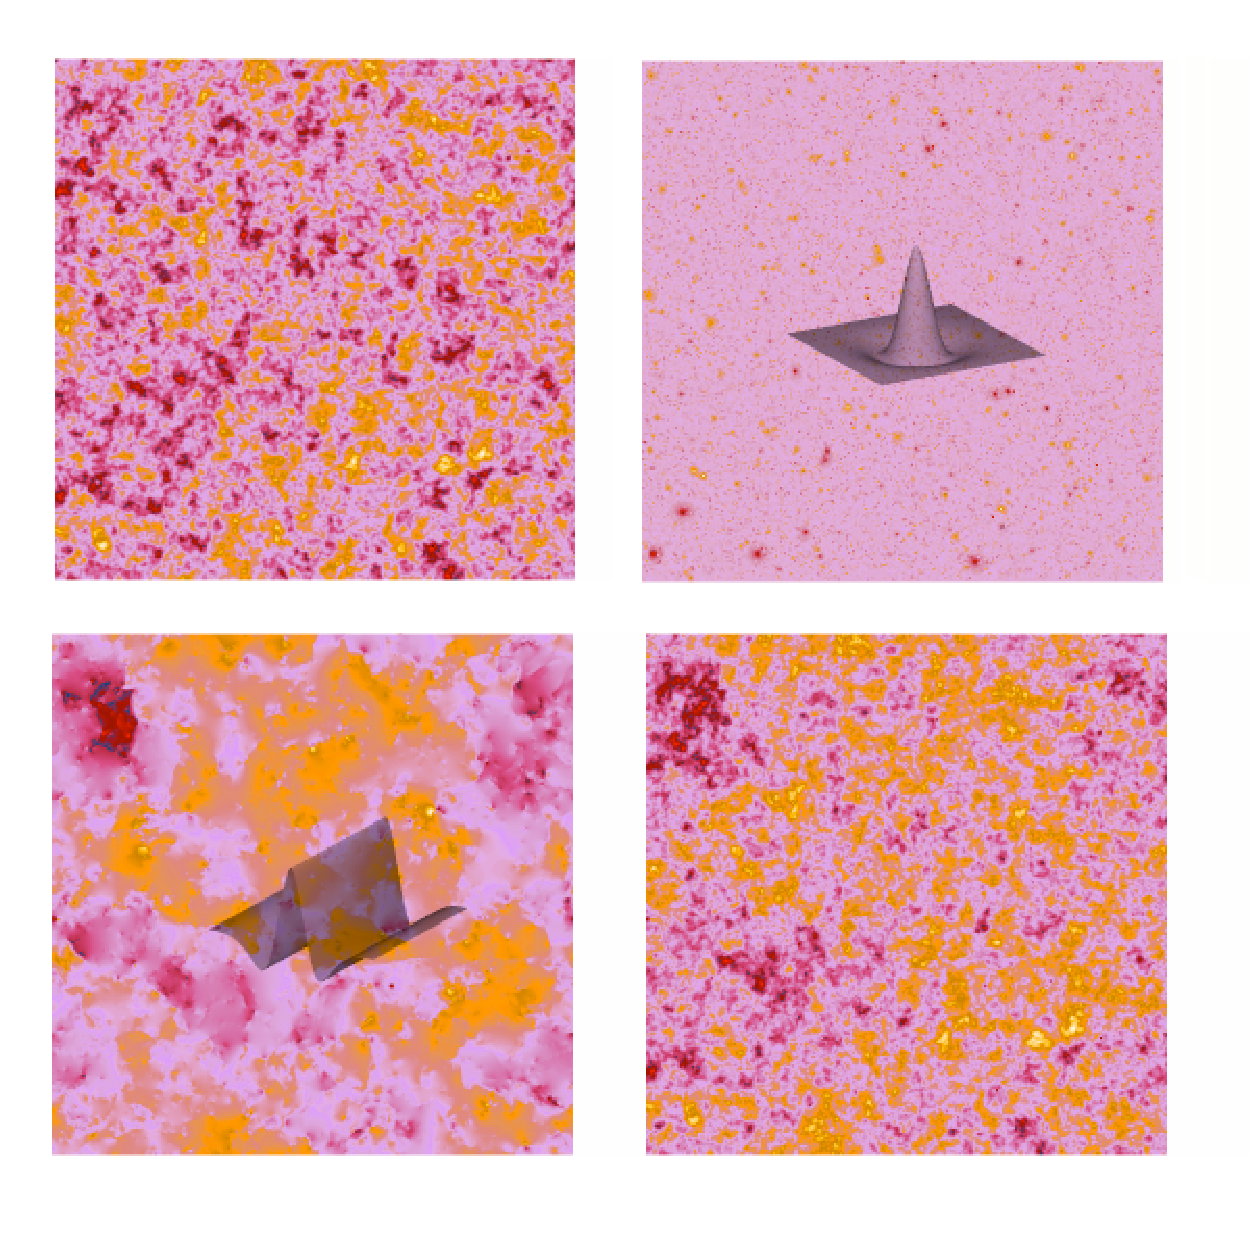
\includegraphics[width=13cm,height=13cm]{fig_cmbcssz.pdf}
\caption{Top, primary Cosmic Microwave Background anisotropies (left) and kinetic Sunyaev-Zel'dovich fluctuations (right). 
Bottom, cosmic string simulated map (left) and simulated observation containing the previous three components (right). 
The wavelet function is overplotted on the Sunyaev-Zel'dovich map and the curvelet function is overplotted on cosmic string map.}
\label{fig_cmb}
\end{figure}

In order to illustrate this, we show in Fig.~\ref{fig_cmb} a set of simulated maps. Primary CMB, kinetic SZ and cosmic string 
maps are shown respectively in Fig.~\ref{fig_cmb} top left, top right and bottom left. The ``simulated observed map", containing 
the three previous components, is displayed in Fig.~\ref{fig_cmb} bottom right. The primary CMB anisotropies dominate all the 
signals except at very high multipoles (very small angular scales). The wavelet function is overplotted on the kinetic Sunyaev-Zel'dovich 
map and the curvelet function is overplotted on cosmic string map.


CMB data are different from other astronomical data sets in the sense that they are not sparse (typical sparse data are stars or/and 
galaxies on top of a smooth background). After a component separation processing (see chapter~\ref{ch_mrs_ica}), the CMB data are not 
completely free of contaminations. Point sources still need to be detected and removed. Once we believe the data are clean enough, 
we want to check if the distribution of CMB temperature fluctuations is Gaussian by using robust statistical Gaussianity tests. 
\index{SZ effect}
\index{cosmic strings}
\index{CMB}

\section{Point Sources on a Gaussian Background}
\index{detection!point sources}
\index{wavelet!mexican hat}
\index{detection!matched filter}

Several methods have been proposed in the last years for point source detection in the CMB such as the the Mexican Hat wavelet \citep{gauss:cayon00,gauss:cayon01}, 
the pseudo-filter \citep{gauss:sanz01}, or the biparametric scale-adaptive filter \citep{gauss:sanz05}. A simple and robust technique, which maximizes 
the signal-to-noise ratio is the Matched Filter \citep{gauss:vio02}. Assuming an isotropic point spread function (PSF) with known power sprectum $\tau(q)$ 
and the CMB with power spectrum $P(q)$, the Matched Filter is \citep{gauss:vio02}:
\begin{equation} 
\label{eqn_mf}
\widehat{\psi}_{MF}(q) = \frac{1}{2 \pi \alpha}~ \frac{\tau(q)}{P(q)},\qquad \alpha \equiv \int_0^{+\infty}q \frac{\tau^2}{P} ~dq
\end{equation}
with minimum variance
\begin{equation} 
\sigma^2 = \frac{1}{2 \pi \alpha}
\end{equation}

\newpage
If the PSF is unknown (or space-variant), the Mexican Hat wavelet may be a good alternative. It consists of convolving the data 
with the wavelet function $\psi_{a,b} (x) =  \psi(\frac{x-b}{a})$, where $\psi(x)= \frac{1}{\sqrt{2\pi}}(1 - x^2) e^{- x^2/2}$. 
$a$ is the scale parameter and $b$ the position parameter. A fast implementation is obtained by using the Fourier transform to 
perform the convolution products ($\widehat{\psi}_{a}(q) = \frac{2}{\sqrt{\pi}} {(q a )}^2 e^{- \frac{1}{2}{(q a)}^2}$) \citep{gauss:sanz05}.




\section{Detecting Faint Non-Gaussian Signals Superposed on a Gaussian Signal}
\label{sec:Theory}
The superposition of a non-Gaussian signal with a Gaussian signal can be modeled as $Y = N + G$, where $Y$ is the observed image, 
$N$ is the non-Gaussian component and $G$ is the Gaussian component. We are interested in using transform coefficients to test 
whether $N \equiv 0$ or not.  

\subsection{Hypothesis Testing and Likelihood Ratio Test (LRT).}  
\label{subsec:LRT}
\index{statistic!LRT}

Transform coefficients of various kinds [Fourier, wavelet, curvelet, etc.] have been used for detecting non-Gaussian behavior 
in numerous studies. Let $X_1, X_2, \ldots, X_n$ be the transform coefficients of $Y$; we model these as  
\begin{equation}    
\label{EqAlt}
X_i = \sqrt{1 - \lam} \cdot  z_i + \sqrt{\lam} \cdot w_i,  \qquad 0< \lam < 1
\end{equation}
where $\lam >0$ is a parameter, $z_i \stackrel{iid}{\sim} N(0,1)$ are the transform coefficients of the Gaussian component $G$, 
$w_i \stackrel{iid}{\sim} W$ are the transform coefficients of the non-Gaussian component $N$, and $W$ is some unknown symmetrical 
distribution. Here without loss of generality, we assume the standard deviation for both $z_i$ and $w_i$ are $1$. 

Phrased in statistical terms, the problem of detecting the existence of a non-Gaussian component is equivalent to discriminating between the hypotheses:  
\begin{eqnarray}
\label{EqHypo2}
&H_0: \;\;\;   X_i = z_i  \label{EqHypo1}   \\
&H_1:   X_i = \sqrt{1 - \lam } \cdot z_i  + \sqrt{\lam} \cdot  w_i,   \qquad 0 < \lam < 1  
\end{eqnarray}
and $N \equiv 0$ is equivalent to $\lam \equiv 0$. We call $H_0$ the {\it null hypothesis $H_0$}, and $H_1$ the {\it alternative hypothesis}. 

% \begin{figure}
% \centering
% \includegraphics[height = 3 in]{PDF/CSDetectRegion.pdf}
% \caption{Detectable regions  in the $\alpha-r$ plane.  With $(\alpha,r)$ in the white region on the top or the undetectable region, all methods completely fail for detection. With $(\alpha,r)$ in the white region on the bottom,  both excess kurtosis and Max/HC are able to detect reliably.      While in the blue region to the left,  Max/HC is able to detect reliably, but excess kurtosis completely fails, and in the yellow region to the right, excess kurtosis is able to detect reliably, but Max/HC  completely fail.     }
% \label{Figure:Detect}
% \end{figure}

\begin{figure}[htb]
\centerline{
\hbox{
\includegraphics[width=12cm]{CSDetectRegion.pdf}%,height=12cm
% \psfig{figure=,bbllx=1.5cm,bblly=8.cm,bburx=19.5cm,bbury=23cm,height=6cm,width=7.5cm,clip=}
 }}
\caption{Detection Boundary in the $\alpha-r$ plane. The solid curve is the detection boundary of LRT, above which is not possible to detect, 
and below which it is possible to reliably detect, the dotted line segment and solid line segment together is the detection boundary for Kurtosis, 
the dotted curve and the solid curve together is the detection boundary of Max/HC. Right panel: detectable regions for Kurtosis, Max/HC.}
\label{Figure:Detect}
\end{figure}

When both $W$ and $\lam$ are known, then the optimal test for Problem (\ref{EqHypo1}) - (\ref{EqHypo2}) is simply 
the Neyman-Pearson Likelihood ratio test (LRT), \cite[Page 74 ]{Lehmann}. The size of $\lam = \lam_n$  for which 
reliable discrimination between $H_0$ and $H_1$ is possible can be derived using asymptotics. If we assume that 
the tail probability of $W$ decays algebraically, 
\begin{equation} \label{EqDefineAlg}
\lim_{x \goto \infty}   x^{\alpha}  P\{|W| > x\}  = C_{\alpha},  \qquad \mbox{$C_{\alpha}$ is a constant}
\end{equation}
(we say $W$ has a power-law tail), and we calibrate $\lam$ to decay with $n$, so that increasing amounts of data are offset by increasingly hard challenges: 
\begin{equation}   \label{EqDefineLam}
\lam = \lam_n  = n^{-r}  
\end{equation}
then there is a {\it threshold effect} for the detection problem (\ref{EqHypo1}) - (\ref{EqHypo2}). In fact, define:\\
\begin{equation} \label{EqDetectBoundary}
\rho^*_1(\alpha) = 
\left\{ \begin{array}{ll}
2/\alpha, &\   \  \alpha \leq 8 \\
1/4, &\     \       \alpha > 8
\end{array}
\right.
\end{equation}
then as $n \goto \infty$, LRT is able to reliably detect for large $n$ when $r < \rho^*_1(\alpha)$, and is unable to detect 
when $r > \rho^*_1(\alpha)$; this is proved in \citep{DJ04b}. Since LRT is optimal, it is not possible for any statistic to 
reliably detect when $r > \rho^*_1(\alpha)$. We call the curve $r = \rho^*_1(\alpha)$ in the $\alpha$-$r$ plane the 
{\it detection boundary}; see Figure \ref{Figure:Detect}.\\

In fact, when $r < 1/4$, asymptotically LRT is able to reliably detect whenever $W$ has a finite $8$-th moment, even without 
the assumption that $W$ has a power-law tail. Of course, the case that $W$ has an infinite $8$-th moment is more complicated, 
but if $W$ has a power-law tail, then LRT is also able to reliably detect if $r < 2/\alpha$. 

% One component of the above result is that, by assuming  $W$ has an 
% $\alpha$-algebraic tail 
% with $\alpha > 8$, then when $r < \frac{1}{4}$,  LRT is 
% able to reliably detect;  
% and when $r > \frac{1}{4}$, no statistic is able to detect.  
% It is interesting to notice here that, this part of the conclusion will still hold 
% when  
% the condition of requiring $W$ to have an algebraic tail is largely relaxed:  in 
% fact,  the same conclusion still holds if we only require $E[W^8] < \infty$.  It is 
% interesting to notice here that,  when $W$ has an $\alpha$-algebraic tail, 
% $E[W^8] < \infty$ if and only if $\alpha > 8$.

Despite its optimality, LRT is not a practical procedure. To apply LRT, one needs to specify the value of $\lam$ and 
the distribution of $W$, which seems unlikely to be available. We need non-parametric detectors, which can be implemented 
without any knowledge of $\lam$ or $W$, and depend on $X_i$'s only. In the next section, we are going to introduce three 
non-parametric detectors: excess kurtosis, Max and Higher Criticism (HC).   

\section{Kurtosis, HC from Wavelet and Curvelet Coefficients}
 
\subsection{Kurtosis}
\index{statistic!Kurtosis}
\index{Kurtosis}

For a statistic $T_n$, the $p$-value is the probability of seeing equally extreme results under the null hypothesis:
\[
p = P_{H_0} \{ T_n  \geq t_n(X_1,X_2, \ldots,X_n) \}
\] 
here $P_{H_0}$ refers to probability under $H_0$, and $t_n(X_1,X_2, \ldots,X_n)$ is the observed value of statistic $T_n$. 
Notice that the smaller the $p$-value, the stronger the evidence against the null hypothesis. A natural decision rule based 
on $p$-values rejects the null when $p < \alpha$ for some selected level $\alpha$, and a convenient choice is  $\alpha = 5\%$. 
When the null hypothesis is indeed true, the $p$-values for any statistic are distributed as uniform $U(0,1)$. This implies 
that the $p$-values provide a common scale for comparing different statistics. 

We now introduce two statistics for comparison. 

{\bf Excess Kurtosis ($\kappa_n$)}. Excess kurtosis is a widely used statistic, based on the $4$-th moment. 
For any (symmetrical) random variable $X$, the kurtosis is:
\[
\kappa(X) = \frac{EX^4}{(EX^2)^2} -3
\]
The kurtosis measures a kind of departure of $X$ from  Gaussianity, as $\kappa(z) =  0$.
Empirically, given $n$ realizations of $X$, the excess kurtosis statistic is defined as: 
\begin{equation}  \label{EqDefineK}
\kappa_n(X_1, X_2,\ldots,X_n)  = \sqrt{\frac{n}{24}} \biggl[ \frac{\frac{1}{n}\sum_i  X_i^4}{(\frac{1}{n}  \sum_i X_i^2)^2}  - 3  \biggr]
\end{equation} 
When the null is true, the excess kurtosis statistic is asymptotically normal:
\[
\kappa_n(X_1, X_2,\ldots,X_n)  \rightarrow_{w}  N(0,1), \qquad n \goto \infty
\]
thus for large $n$, the $p$-value of the excess kurtosis is approximately:
\[
\tilde{p} = \bar{\Phi}^{-1} (\kappa_n(X_1, X_2,\ldots,X_n))
\]
where $\bar{\Phi}(\cdot)$ is the survival function (upper tail probability) of $N(0,1)$. 

It is proved in \citep{DJ04b} that the excess kurtosis is asymptotically optimal for the hypothesis testing of \eqref{EqHypo1} - \eqref{EqHypo2} if 
\[
E [W^8] < \infty
\]
However, when $E[W^8] = \infty$, even though kurtosis is well-defined ($E[W^4] < \infty$), there are situations in which LRT 
is able to reliably detect but excess kurtosis completely fails. In fact, by assuming \eqref{EqDefineAlg} - \eqref{EqDefineLam} 
with an $\alpha < 8$, if $(\alpha,r)$ falls into the blue region of Figure~\ref{Figure:Detect}, then LRT is able to reliably detect, 
however, excess kurtosis completely fails. This shows that in such cases, excess kurtosis is not optimal; see \citep{DJ04b}. 

\subsection{Max}
\index{statistic!max}
\index{max}
The largest (absolute) observation is a classical and frequently-used non-parametric statistic:
\[
M_n =  \mmax(|X_1|,|X_2|,\ldots, |X_n|)
\] 
under the null hypothesis, 
\[
M_n  \approx \sqrt{2 \log n}
\]
and moreover, by normalizing $M_n$ with constants $c_n$ and $d_n$, the resulting statistic 
converges to the Gumbel distribution $E_v$, whose cdf is $e^{-e^{-x}}$:
\[
\frac{M_n - c_n}{d_n}  \rightarrow_{w}    E_v
\]
where approximately
\[
d_n = \frac{\sqrt{6} S_n}{\pi}, \qquad  c_n = \bar{X} - 0.5772 d_n 
\]
here $\bar{X}$ and $S_n$ are the sample mean and sample standard deviation of $\{X_i\}_{i=1}^n$ respectively. 
Thus a good approximation of the $p$-value for $M_n$ is:
\[
\tilde{p} =  \mathrm{exp}(-\mathrm{exp}(-\frac{M_n - c_n}{d_n}))
\]
We have tried the above experiment for $n = 244^2$, and found that taking $c_n = 4.2627$, $d_n = 0.2125$ gives a good approximation.  

Assuming \eqref{EqDefineAlg} - \eqref{EqDefineLam} and $\alpha < 8$, or $\lam = n^{-r}$ and that $W$ has a power-law tail 
with $\alpha < 8$, it is proved in \citep{DJ04b} that Max is optimal for hypothesis testing \eqref{EqHypo1} - \eqref{EqHypo2}. 
Recall if we further assume $\frac{1}{4} < r < \frac{2}{\alpha}$, then asymptotically, excess kurtosis completely fails; 
however, Max is able to reliably detect and is competitive to LRT. 

On the other hand, recall that excess kurtosis is optimal for the case $\alpha > 8$. In comparison, in this case, 
Max is not optimal. In fact, if we further assume $ \frac{2}{\alpha} < r < \frac{1}{4}$, then  excess kurtosis 
is able to reliably detect, but Max will completely fail. 

In Figure \ref{Figure:Detect}, we compared the detectable regions of the excess kurtosis and Max in the $\alpha$-$r$ plane. 

\subsection{Higher Criticism}
\label{sec:HC}
\index{statistic!Higher Criticism}
\index{Higher Criticism}

The Higher Criticism statistic (HC), was proposed in \citep{gauss:lin02}. To define HC first we convert the individual $X_i$'s 
into $p$-values for individual $z$-tests. Let $p_i = P\{ N(0,1) > X_i \}$ be the $i^{th}$ $p$-value, and let $p_{(i)}$ denote 
the $p$-values {\it sorted in increasing order}; the Higher Criticism statistic is defined as:
\[
       HC_{n}^* =  \max_{i}
         \biggl| \sqrt{n} [i/n  - p_{(i)}]/ \sqrt{p_{(i)} (1-p_{(i)})} \biggr|
\]
or in a modified form:
\[
HC_n^+  = \max_{\{i:  \; 1/n  \leq  p_{(i)} \leq  1 - 1/n \}}
         \biggl|   \sqrt{n} [i/n  - p_{(i)}]/ \sqrt{p_{(i)} (1-p_{(i)})}  \biggr|
\]
we let $HC_n$ refer either to $HC_n^*$ or $HC_n^+$ whenever there is no confusion. The above definition is slightly 
different from \citep{gauss:lin02}, but the ideas are essentially the same.

With an appropriate normalization sequence:
\[
a_n = \sqrt{2 \log \log n}, \qquad b_n = 2 \log \log n + 0.5 \log \log \log n - 0.5 \log (4 \pi)
\]
the distribution of $HC_n$ converges to  the Gumbel distribution $E_v^4$, whose cdf is $\mathrm{exp}(-4\mathrm{exp}(-x))$, \citep{Shorack}:
\[
a_n  HC_n - b_n  \rightarrow_w  E_v^4
\]
so the $p$-values of $HC_n$ are approximately:
\begin{equation}  
\label{EqHCP}
\mathrm{exp}(-4\mathrm{exp}( - [a_n HC_n - b_n]))
\end{equation}
For moderately large $n$, in general, the approximation in \eqref{EqHCP} is accurate for the $HC_n^+$, but not for $HC_n^*$.   

A brief remark comparing Max and HC. Max only takes into account the few largest observations, HC takes into account those outliers, 
but also moderate large observations. As a result, in general HC is better than Max, especially when we have unusually many moderately 
large observations. However, when the actual evidence lies in the middle of the distribution both HC and Max will be very weak.

% \section{The Genus and the Multiscale Genus}

\section{Experiments}

\begin{figure}[htb]
\vbox{
\centerline{
\hbox{
 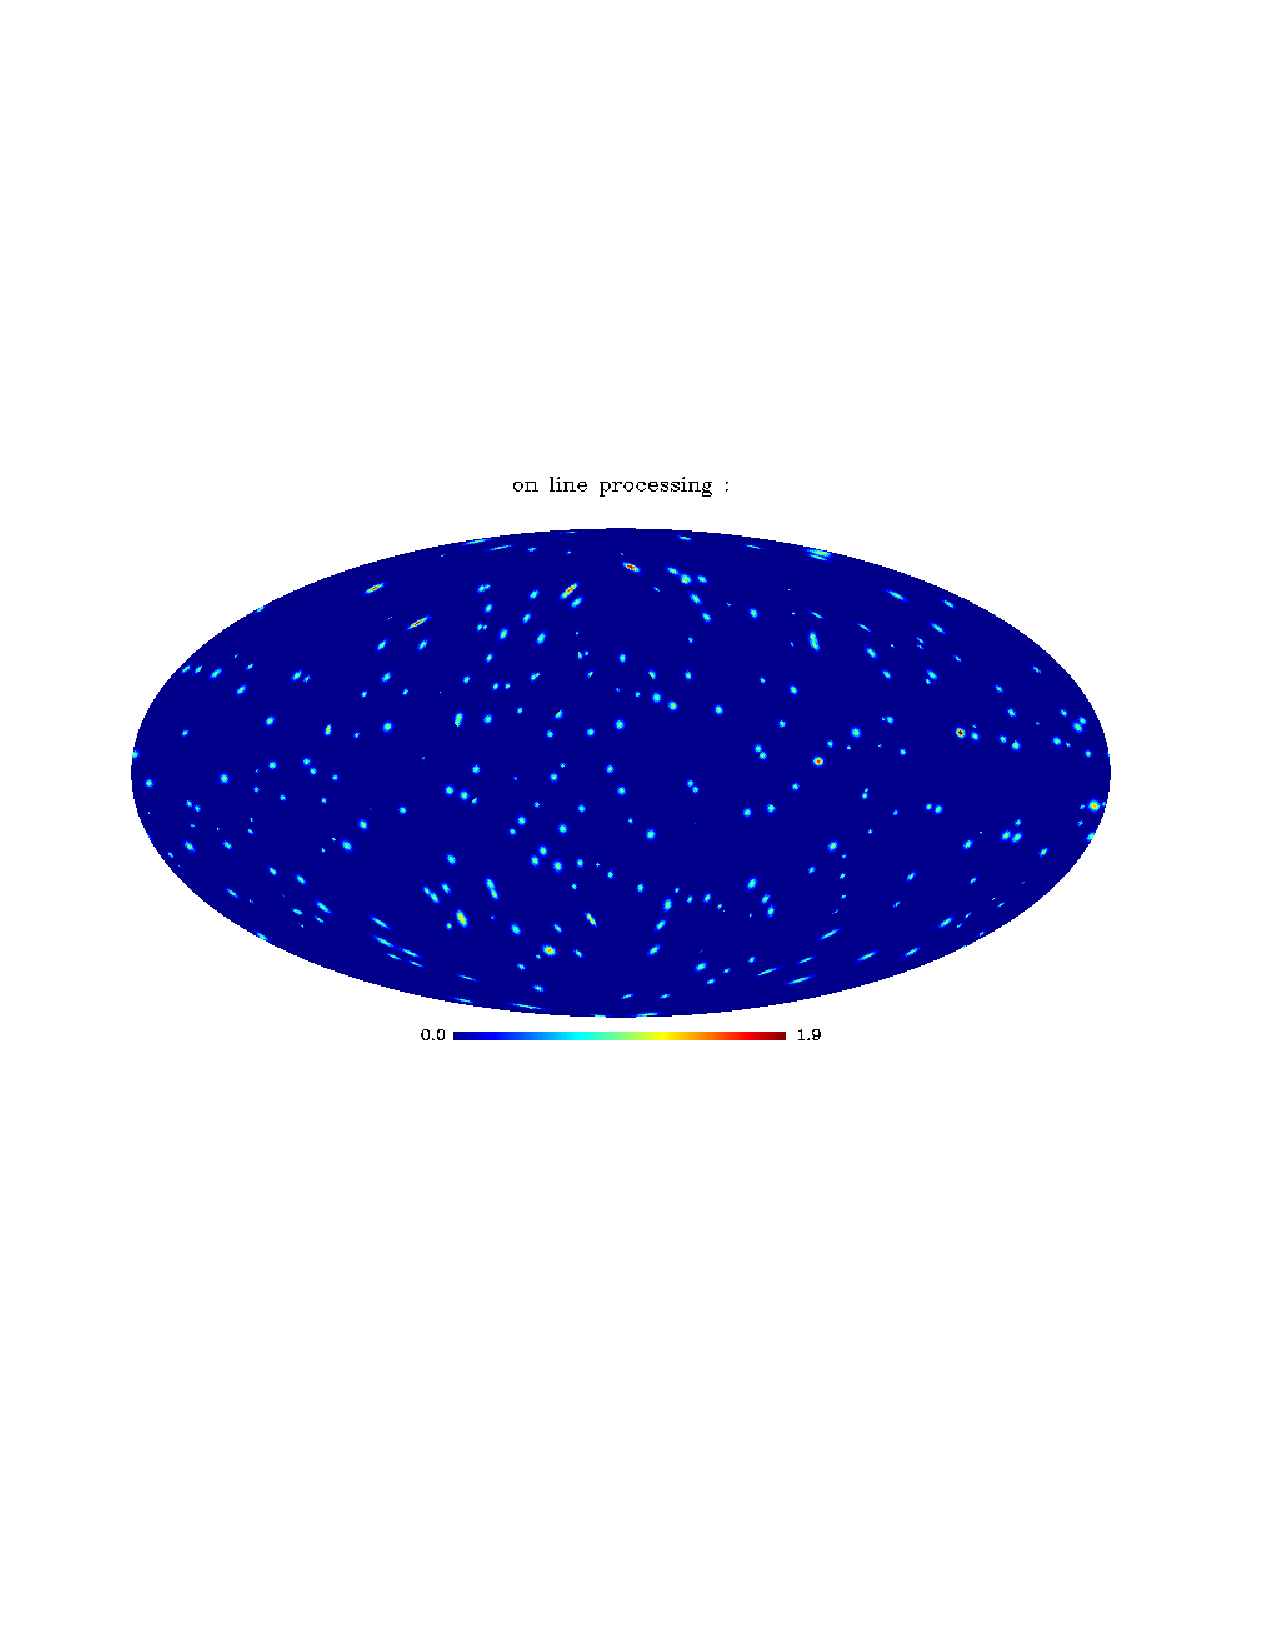
\includegraphics[trim= 2cm 8cm 2cm 8cm,width=7.9cm]{fig_sphere_gaussian.pdf}%[width=8.5cm,height=4.5cm]
 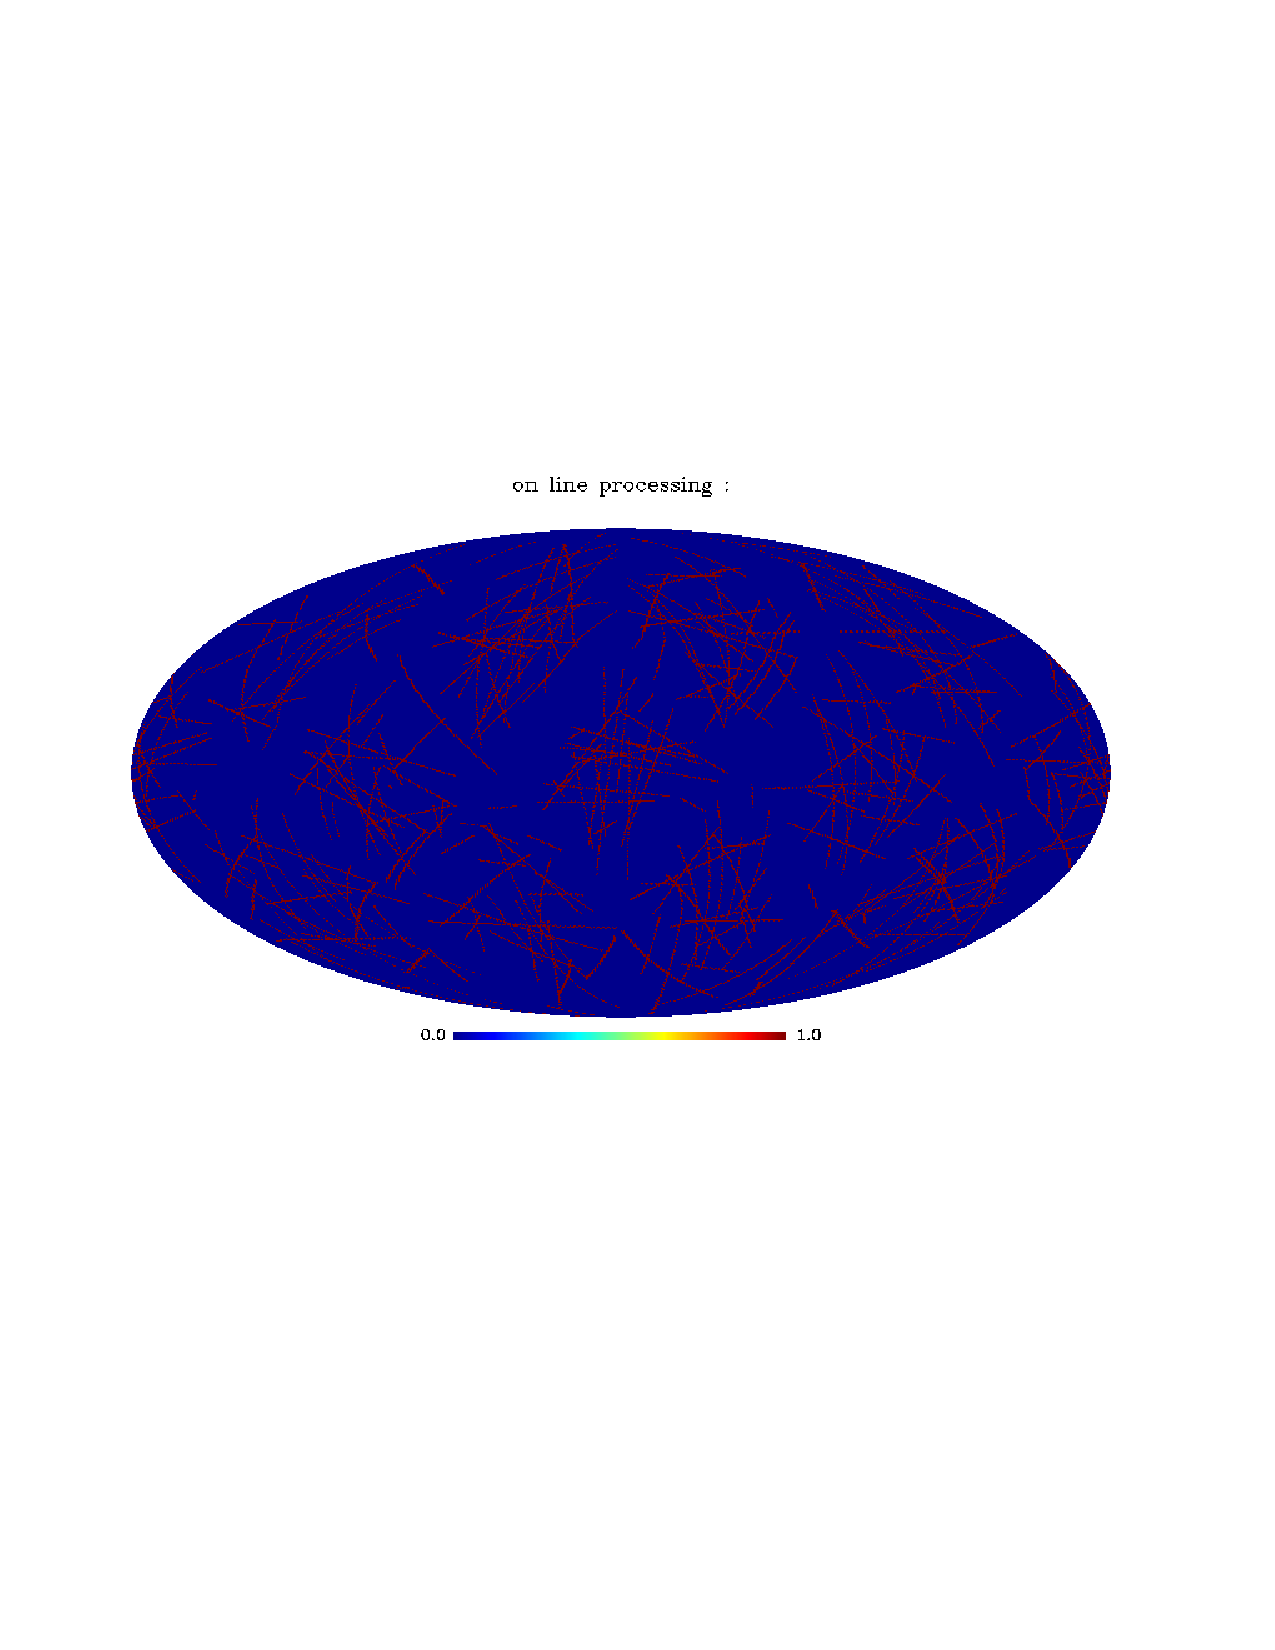
\includegraphics[trim= 2cm 8cm 2cm 8cm,width=7.9cm]{fig_sphere_line.pdf}
}}
 \centerline{
 \hbox{
 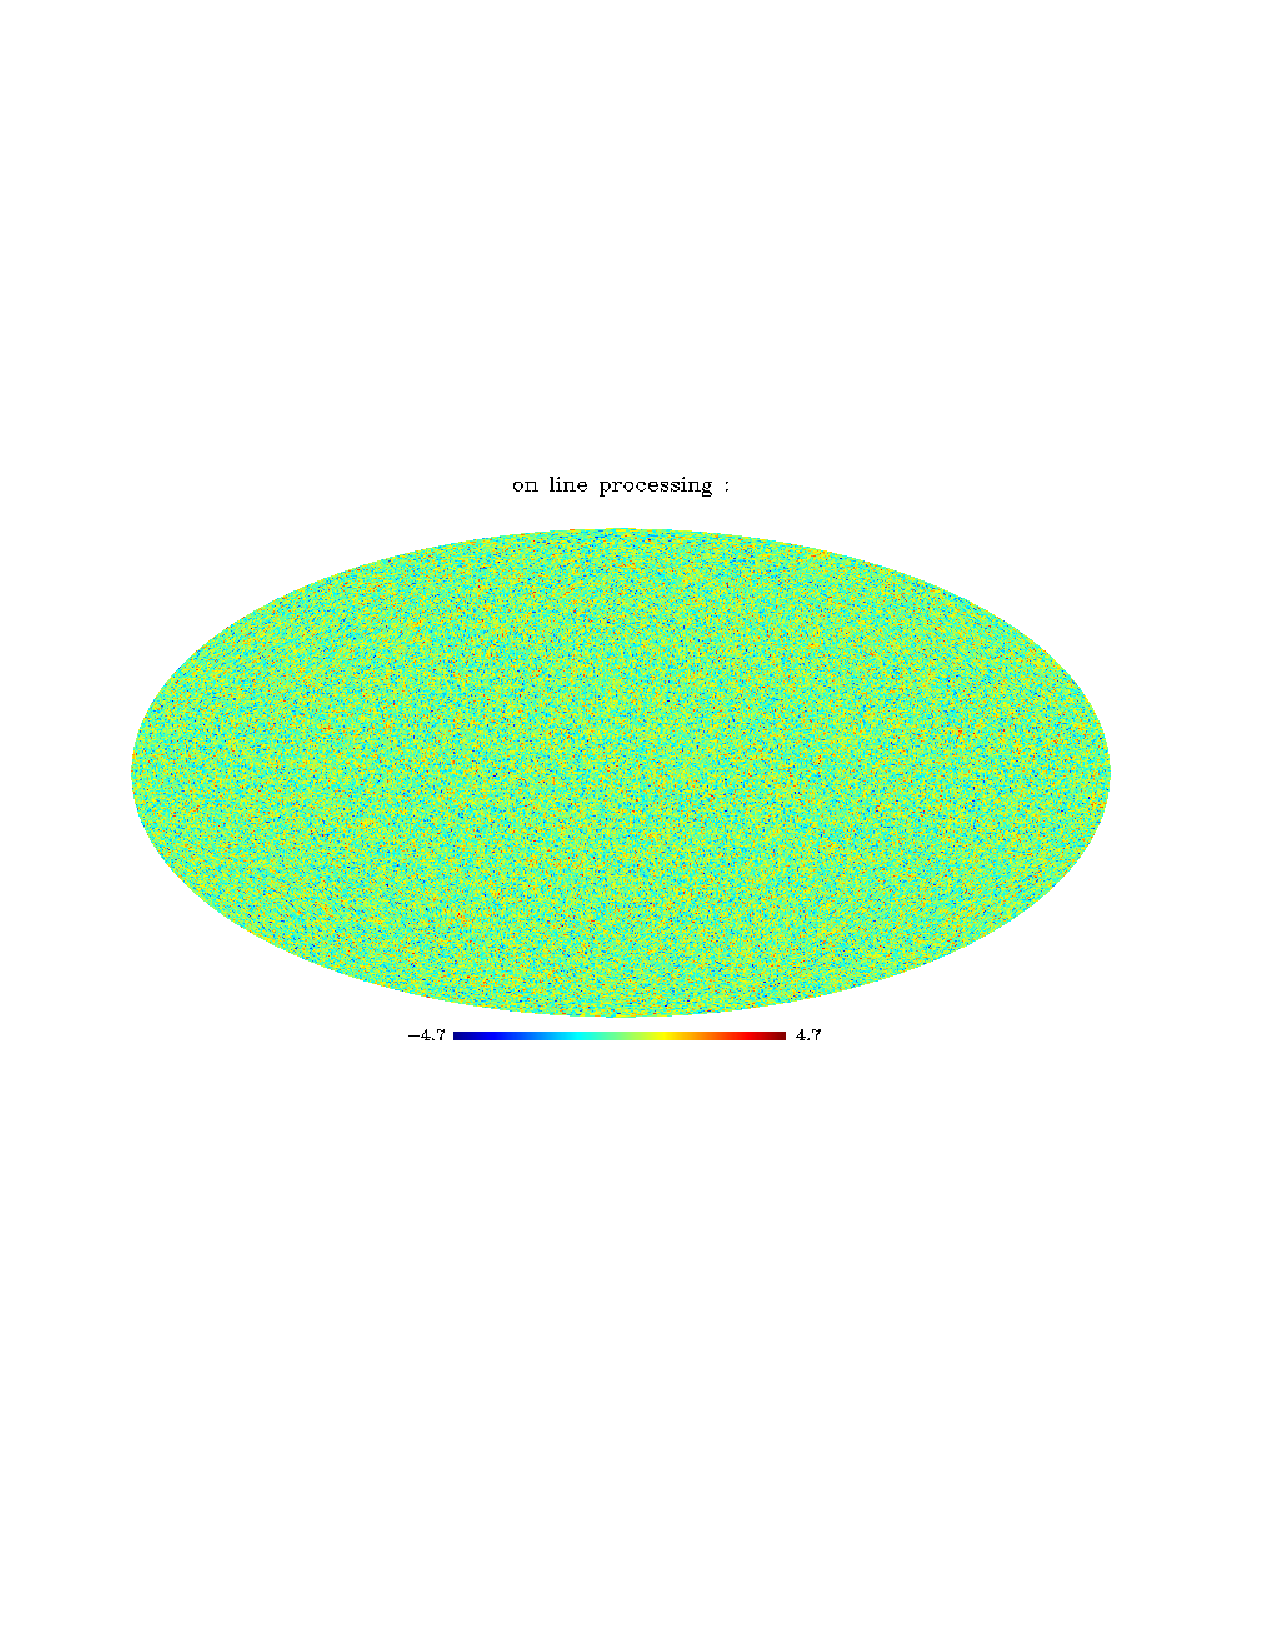
\includegraphics[trim= 2cm 8cm 2cm 8cm,width=7.9cm]{fig_sphere_gaussian_noise_snr1.pdf}
 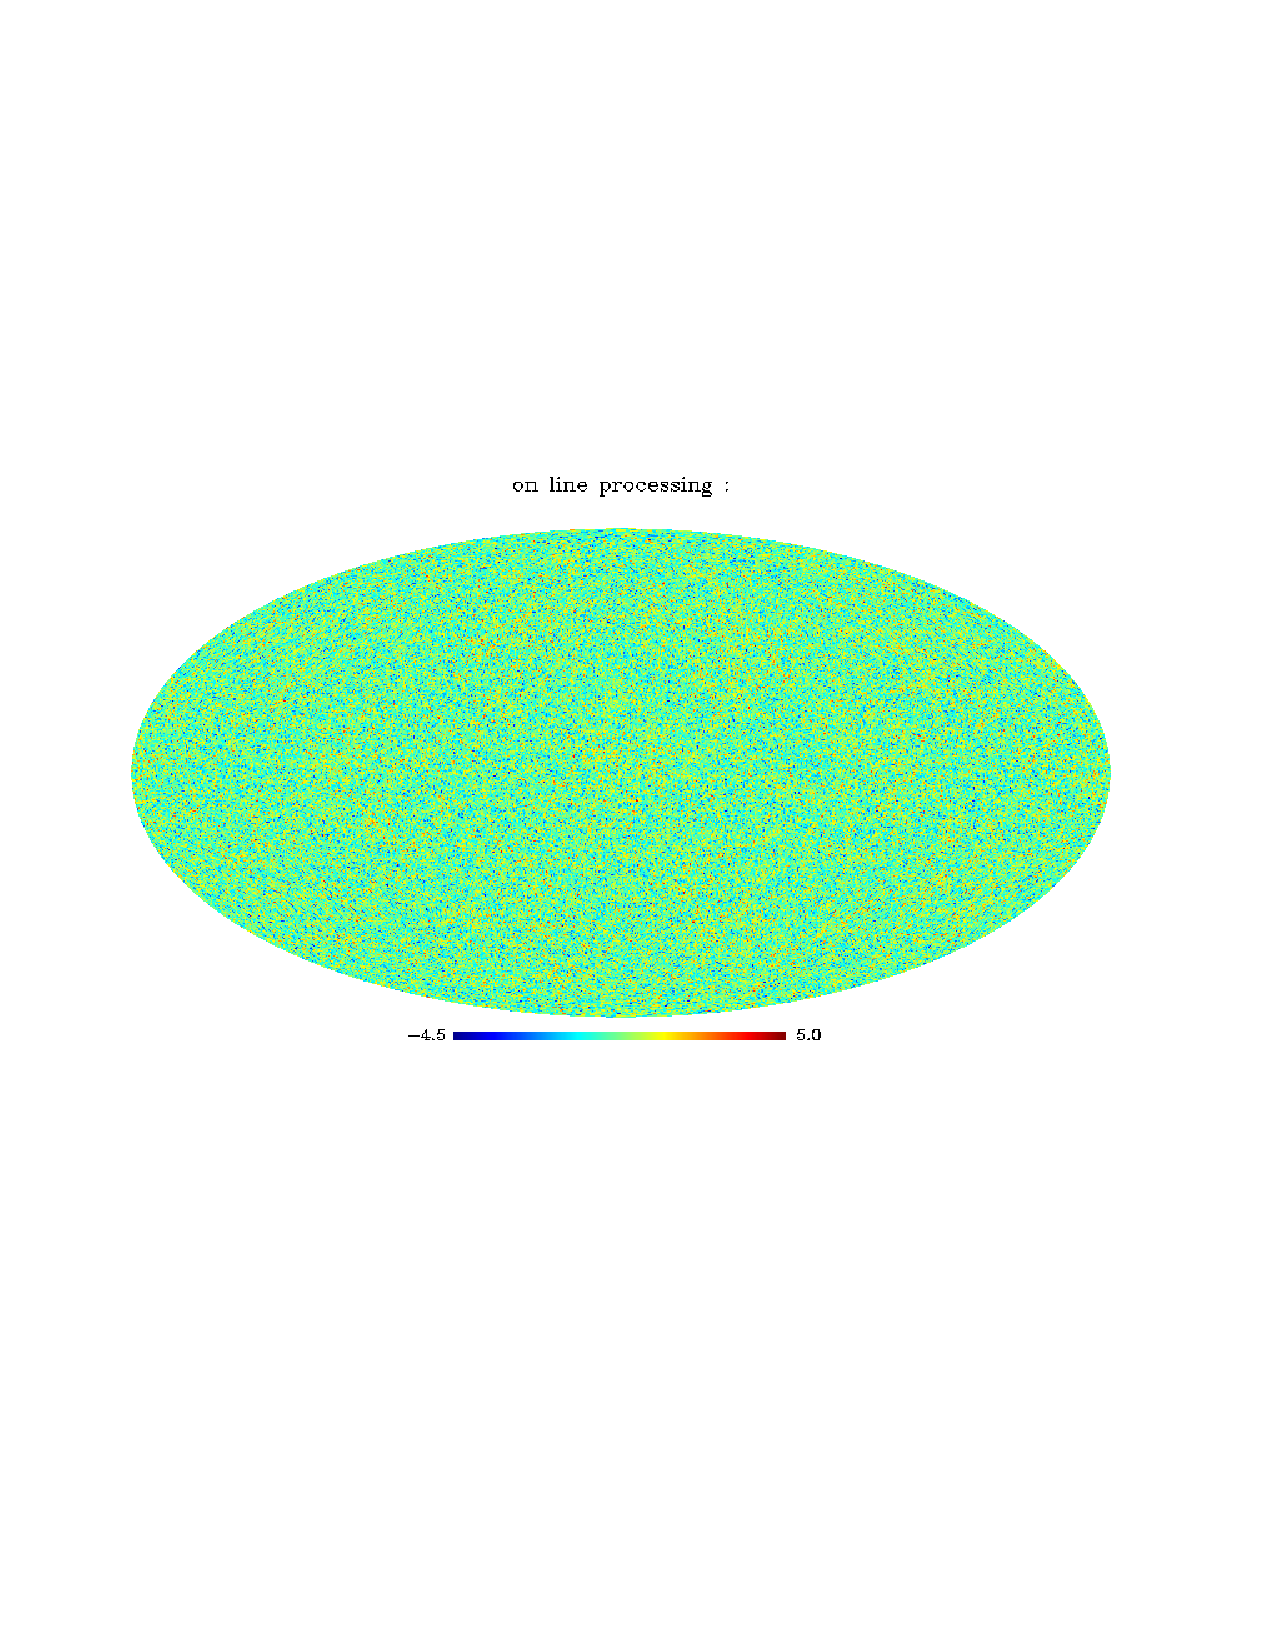
\includegraphics[trim= 2cm 8cm 2cm 8cm,width=7.9cm]{fig_sphere_line_noise_snr1.pdf}
}}}
 \caption{Top, image with Gaussians and image with lines. Bottom, same images but with an additional Gaussian noise. The SNR is equal to 1.}
\label{fig_sphere_linegauss}
\end{figure}

Fig.~\ref{fig_sphere_linegauss} shows, top left and right, two images with respectively Gaussians and lines. We have created a set 
of simulated images by adding a Gaussian white noise with different standard deviations to these two images. The Signal to Noise 
Ratio (SNR) varies between 0 and 1. For the image with lines, the SNR is defined as the pixel values along the lines divided by the 
noise standard deviation, and  for the image with Gaussians, the SNR is defined as the maximum of the Gaussians divided by the noise 
standard deviation. Fig.~\ref{fig_sphere_linegauss} shows, bottom left and right, the two noisy images with a SNR equal to 1. Hence, 
for each SNR value, we have thirty realizations of the noise, and we have calculated the kurtosis at the different scales of both the 
curvelet and the wavelet coefficients. These kurtosis values were normalized by the standard deviation of the kurtosis obtained from 
the wavelet and the curvelet transform of thirty Gaussian white noise realizations. Finally we kept for each SNR the maximum normalized 
kurtosis along the scales. Fig.~\ref{fig_wtcur_sphere_linegauss} left (resp.~right) shows the normalized kurtosis values using the wavelet 
transform (resp. the curvelet transform) for the two images (i.e. lines and Gaussians) versus the SNR. Continuous error bars correspond 
to $1\sigma$ level and dashed error bars correspond to $2\sigma$ level. We can clearly see that the detection power of the wavevet 
transform is much larger than the detection power of the curvelet transform for detecting non-Gaussianities due to isotropic features, 
while curvelets are more powerful than wavelets for detecting anisotropic features.

\begin{figure}[htb]
\centerline{
 \hbox{
% {figure=,bbllx=2.5cm,bblly=12.5cm,bburx=19.5cm,bbury=25.5cm,width=8.5cm,height=6.5cm,clip=}
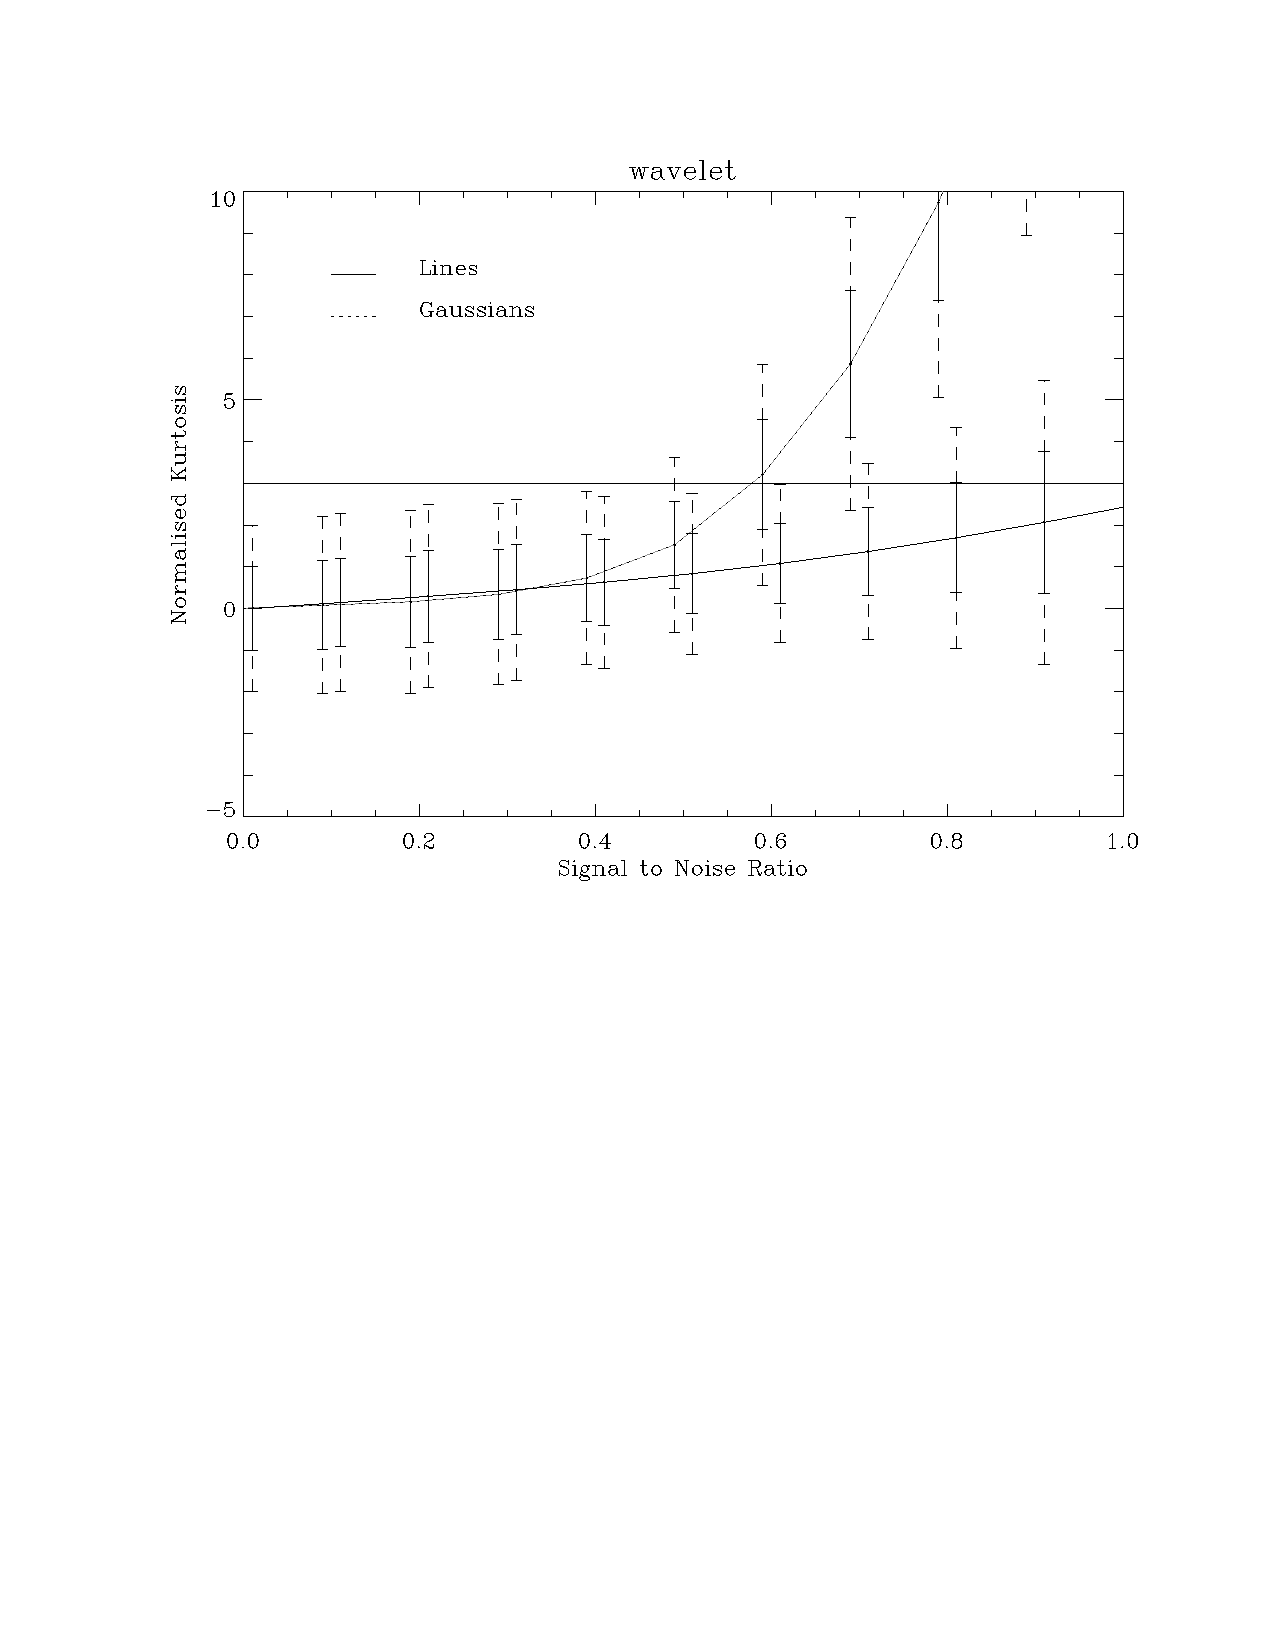
\includegraphics[trim= 2cm 13cm 2cm 3cm,width=7.9cm]{fig_sphere_wt_linedroite.pdf}%,height=6.5cm
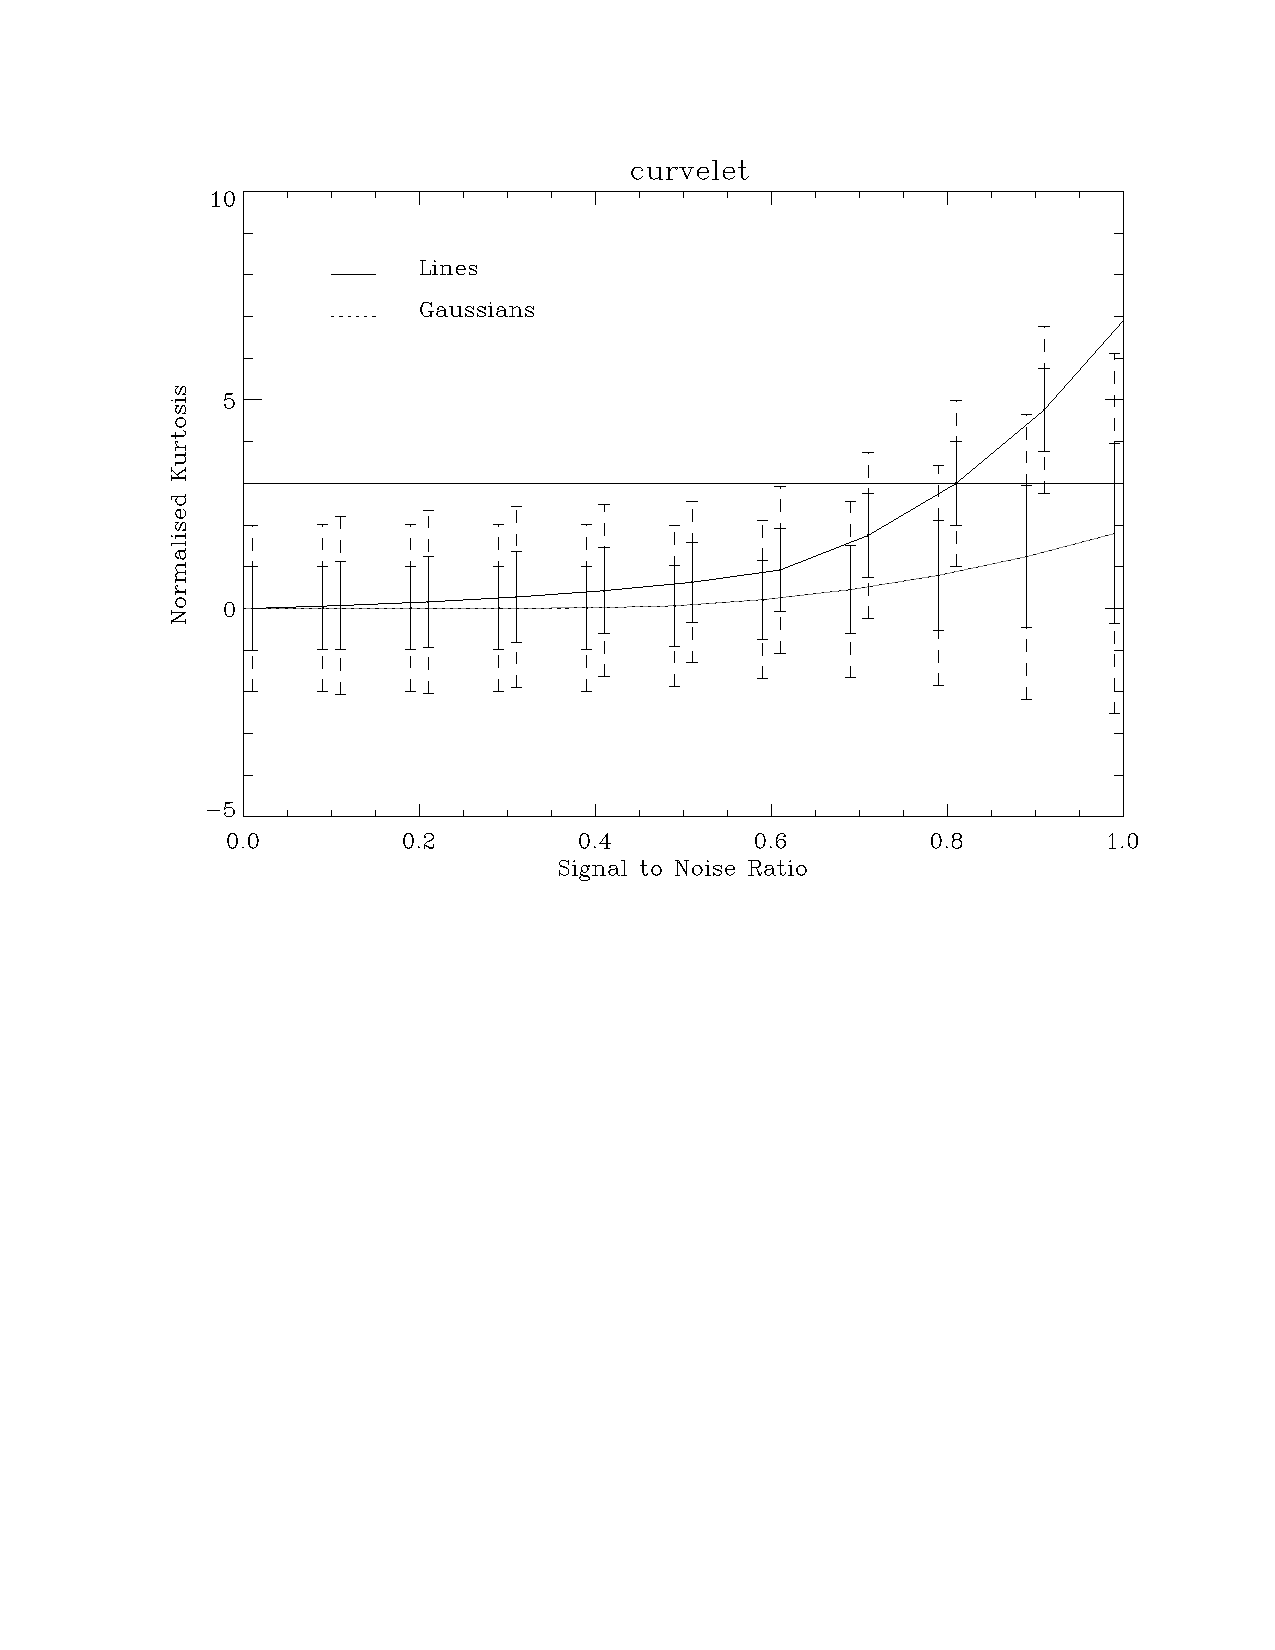
\includegraphics[trim= 2cm 13cm 2cm 3cm,width=7.9cm]{fig_sphere_cur_linedroite.pdf}
% \psfig{figure=fig_sphere_cur_linedroite.pdf,bbllx=2.5cm,bblly=12.5cm,bburx=19.5cm,bbury=25.5cm,width=8.5cm,height=6.5cm,clip=}
}}
\caption{Normalised kurtosis value versus the SNR for the wavelet coefficients (left) and the curvelet coefficients (right). 
The continuous error bars correspond to one $\sigma$ and the dashed error bars correspond to $2\sigma$.}
\label{fig_wtcur_sphere_linegauss}
\end{figure}

\section{Conclusions}
\index{wavelet!Kurtosis}
\index{wavelet!Higher Criticism}
\index{curvelet!Kurtosis}
\index{curvelet!Higher Criticism}
\index{SZ effect}
\index{cosmic strings}
\index{detection!non-Gaussianity}

The kurtosis of the wavelet coefficients is very often used in astronomy for the detection of non-Gaussianities in the CMB. It has been 
shown \citep{starck:sta03_1} that it is also possible to separate the non-Gaussian signatures associated with cosmic strings from those 
due to SZ effect by combining the excess kurtosis derived from these both the curvelet and the wavelet transform. It has been shown that 
kurtosis is asymptotically optimal in the class of weakly dependent symmetric non-Gaussian contamination with finite 8-th moments, while 
HC and MAX are asymptotically optimal in the class of weakly dependent symmetric non-Gaussian contamination with infinite 8-th moment \citep{starck:jin05}. 
Hence depending on the nature of the non-Gaussianity, a statitic is better than another one. This is a motivation for using several statistics 
rather than a single one for analysing CMB data. The case of the detection of cosmic string contaminations has been studied on simulated maps, 
and it has been shown that kurtosis outperforms clearly Max/HC \citep{starck:jin05}.  






\chapter{Multiscale Entropy as a Measure of Relevant Information in an Image}
 
Since the multiscale entropy extracts the information from the signal only, 
it was a  challenge to see if the  astronomical content of  an image
was related to its multiscale entropy.

For this purpose, we studied the astronomical content of 200 images 
of 1024 $\times$ 
1024 pixels extracted from scans of 8 different plates carried out  
by the MAMA facility (Paris, France) 
\cite{astro:guibert92} and stored at CDS (Strasbourg, France) 
in the Aladin
archive \cite{compress:bonnarel99}. We estimated the content of these images 
in three different ways:
\begin{enumerate}     
\item By counting the number of objects in an astronomical catalog
(USNO A2.0 catalog)   
within the image. The
 USNO (United States Naval Observatory) 
catalog was obtained by source extraction from the same survey 
 plates as we used in our study.
\item By counting the number of objects estimated in the image by the
 Sextractor object detection 
package \cite{astro:bertin96}. As in the case of USNO 
these detections are mainly point sources (stars, as opposed to 
spatially extended objects like galaxies).
\item  By counting the number of structures detected at several scales using 
 the MR/1 multiresolution analysis package \cite{starck:mr1_99}.
\end{enumerate}

\begin{figure}[htb]
\centerline{
\vbox{
\psfig{figure=fig_cds_pmm_entropy.ps,bbllx=2.8cm,bblly=2.8cm,bburx=20.5cm,bbury=15.4cm,width=10cm,height=6cm,clip=}
\psfig{figure=fig_cds_sext_entropy.ps,bbllx=2.8cm,bblly=2.8cm,bburx=20.5cm,bbury=15.4cm,width=10cm,height=6cm,clip=}
\psfig{figure=fig_cds_support_entropie.ps,bbllx=2.8cm,bblly=2.8cm,bburx=20.5cm,bbury=15.4cm,width=10cm,height=6cm,clip=}
}}
\caption{Multiscale entropy versus the number of objects: the number
of objects is, respectively, obtained from (top) the USNO catalog, (middle)
the Sextractor package, and (bottom) the MR/1 package.}
\label{fig_cds_entropy}
\end{figure}

Figs.~\ref{fig_cds_entropy} show the results of plotting these numbers 
for each image against the multiscale signal entropy of the image. 
The best results are obtained using the MR/1 package, 
 followed by Sextractor and then by the number of sources extracted
 from USNO. Of course the latter two basically miss the content
at large scales, which is taken into account by MR/1.

Sextractor and multiresolution methods were also applied to a set of CCD 
images from CFH UH8K, 2MASS and DENIS near infrared surveys.
Results obtained were very similar to what was obtained above.  This seems
to point to multiscale entropy as being a universal measurement of image 
content.

Subsequently we looked for the relation between the multiscale entropy and 
the optimal compression
rate of an image which we can obtain by multiresolution 
techniques \cite{starck:book98}. 
 By optimal compression rate we mean 
a compression rate which allows all the sources to be preserved, and which 
does not
degrade the astrometry and photometry.
Louys et al.\ \cite{starck:louys99}  and Couvidat \cite{compress:couvidat99}
have  estimated   this optimal
compression rate using the compression program of the 
MR/1 package  \cite{starck:mr1_99}.

\begin{figure}[htb]
\centerline{
\hbox{
\psfig{figure=fig_cds_taux.ps,bbllx=2.8cm,bblly=2.8cm,bburx=20.5cm,bbury=15.4cm,width=10cm,height=6cm,clip=}
}}
\caption{Multiscale entropy of astronomical images versus the optimal
compression ratio. Images which contain a high number of sources have
a small ratio and a high multiscale entropy value. The relation 
is almost linear.}
\label{fig_cds_taux}
\end{figure}

Fig.~\ref{fig_cds_taux} shows the relation obtained 
between the multiscale entropy and the optimal compression rate
for all the images used in our previous tests including CCD ones. 
The power law  relation is obvious thus allowing us to conclude that:
\begin{itemize}
\item  The compression rate depends strongly on the astronomical content 
of the image. We can then say that compressibility is 
also an estimator of the content of the image.
\item The multiscale entropy allows us to predict the optimal 
compression rate of the image.
\end{itemize}



% \section{Mutual Information}
\newpage
\chapter{Conclusion}
 
 - To be completed -
 
\clearpage
\newpage


% 
\chapter{\projmw Programs}
\label{ch_prog_mw}
\markright{Programs}

\section{Probability in wavelet space: mw\_proba}
\index{mw\_proba}
The program 
{\em mw\_proba} computes the probability of each wavelet coefficient to be
due to signal (i.e.\ not due to noise).
{\bf 
\begin{center}
 USAGE: mw\_proba options image\_in mr\_file\_out
\end{center}}
where options are~:
\begin{itemize}
\baselineskip=0.4truecm
\itemsep=0.1truecm
\item {\bf [-t type\_of\_multiresolution\_transform]} 
\item {\bf [-m type\_of\_noise]}
\item {\bf [-g sigma]}
\item {\bf [-c gain,sigma,mean]}
\item {\bf [-n number\_of\_scales]}
\item {\bf [-S SizeBlock]} \\
\item {\bf [-N NiterSigmaClip]} \\
\item {\bf [-R RMS\_Map\_File\_Name]} \\
\end{itemize}

\subsubsection*{Examples:}
\begin{itemize}
\item mw\_prob image\_in.d MR\_File\_out.mr \\
Compute the probability of each wavelet coefficient of an image
to be due to signal (i.e. not due to noise).
\item mr\_extract -s 1 MR\_File\_out.mr  scale1.d \\
Create an image from the first scale of the multiresolution file.
\end{itemize}

\section{Entropy of an image: mw\_entrop}
\index{mw\_entrop}
The program 
{\em mw\_entrop} computes the information (entropy) and the signal information
of an image (N1-MSE approach). The two output files mr\_file1\_out and mr\_file2\_out 
are multiresolution files (``.mr'') which contain respectively 
the information and the signal information 
relative to the wavelet coefficients. The program calculates and prints to
the screen the mean entropy and signal entropy per band.
{\bf 
\begin{center}
 USAGE: mw\_entrop options image\_in  mr\_file1\_out mr\_file2\_out
\end{center}}
where options are:
\begin{itemize}
\baselineskip=0.4truecm
\itemsep=0.1truecm
\item {\bf [-t type\_of\_multiresolution\_transform]} 
\item {\bf [-m type\_of\_noise]}
\item {\bf [-g sigma]}
\item {\bf [-c gain,sigma,mean]}
\item {\bf [-n number\_of\_scales]}
\item {\bf [-S SizeBlock]} 
\item {\bf [-N NiterSigmaClip]}
\item {\bf [-R RMS\_Map\_File\_Name]}
\end{itemize}
\subsubsection*{Example:}
\begin{itemize}
\item mw\_entrop image\_in.d MR\_File1\_out.mr MR\_File2\_out.mr \\
Compute the multiscale entropy of an image
\end{itemize}

\section{Filtering}
\subsection{1D filtering: mw1d\_filter}
\index{mw1d\_filter}
The program {\em mw1d\_filter} filters a one dimensional signal using the 
multiscale entropy method (N2-MSE approach). 
{\bf 
\begin{center}
 USAGE: mw1d\_filter options signal\_in  signal\_out
\end{center}}
where options are~:
\begin{itemize}
\baselineskip=0.4truecm
\itemsep=0.1truecm
\item {\bf [-t type\_of\_multiresolution\_transform]} 
\item {\bf [-m type\_of\_noise]}
\item {\bf [-g sigma]} 
\item {\bf [-c gain,sigma,mean]}
\item {\bf [-s NSigma]} 
\item {\bf [-n number\_of\_scales]} 
\item {\bf [-e epsilon]} \\
Convergence parameter. Default is $1e^{-4}$.
\item {\bf [-i number\_of\_iterations]} \\
Maximum number of iterations. Default is 10.
\item {\bf [-G RegulParam]} \\
Regularization parameter. Default is 1.
\item {\bf [-D]} \\
The regularization parameter is a function of the SNR in the data.
Default is no.
\item {\bf [-w FilterCoefFileName]} \\
Write to  disk the filtered wavelet coefficient.
\item {\bf [-v]} \\
Verbose. Default is no.
\end{itemize}

\subsubsection*{Examples:}
\begin{itemize}
\baselineskip=0.4truecm
\itemsep=0.1truecm
\item mw1d\_filter sig\_in.fits sig\_out.d \\
filters a signal by the multiscale entropy method, assuming
Gaussian noise (its standard deviation is automatically estimated).
\item mw1d\_filter -G 2 sig\_in.fits sig\_out.fits \\
Same as before, but the regularization will be stronger, and the solution
more smooth.  
\item mw1d\_filter -G 2 -D sig\_in.fits sig\_out.fits \\
The regularization is adaptive, depending on the wavelet SNR.
\item mw\_filter -G 2 -D -s 5 sig\_in.fits sig\_out.fits \\ 
Same as before, preserving  feature in the wavelet space greater than
$5\sigma$ instead of the default $3\sigma$ value.
\end{itemize}


\subsection{2D filtering: mw\_filter}
\index{mw\_filter}
The program {\em mw\_filter} filters an image using the 
multiscale entropy method (N2-MSE approach). 
{\bf 
\begin{center}
 USAGE: mw\_filter options image\_in image\_out
\end{center}}
where options are:
\begin{itemize}
\baselineskip=0.4truecm
\itemsep=0.1truecm
\item {\bf[-T Type\_of\_Regularization]}
\begin{enumerate}
\baselineskip=0.4truecm
\itemsep=0.1truecm
\item Use a fixed user Alpha value.
\item Estimate the optimal Alpha.
\item Estimate one  Alpha value per band.
\end{enumerate}
Default is 1.
\item {\bf [-D]} \\
Wavelet coefficients with a high signal to noise ratio are not
regularized. For a lower SNR, the Alpha parameter is modified using the SNR.
Default is no regularization.
\item {\bf [-t type\_of\_multiresolution\_transform]} 
\item {\bf [-m type\_of\_noise]} \\
Noise models 1 to 9 are available.
\item {\bf [-g sigma]} 
\item {\bf [-c gain,sigma,mean]}
\item {\bf [-s NSigma]} 
\item {\bf [-S SizeBlock]} 
\item {\bf [-N NiterSigmaClip]} 
\item {\bf [-R RMS\_Map\_File\_Name]} 
\item {\bf [-n number\_of\_scales]} 
\item {\bf [-e epsilon]} \\
Convergence parameter. Default is $1e^{-4}$.
\item {\bf [-i MaxIter]} \\
Maximum number of iterations. Default is 20.
\item {\bf [-G RegulParam]} \\
Regularization parameter. Default is 1.
\item {\bf [-C]} \\
Convergence parameter. Only used when regularization type is equal to
2 or 3.
Default is $0.01$.
\item {\bf [-P]} \\
Apply the positivity constraint. If set, the solution cannot have negative 
values.
\item {\bf [-v]} \\
Verbose. Default is no.
\end{itemize}

\subsubsection*{Examples:}
\begin{itemize}
\baselineskip=0.4truecm
\itemsep=0.1truecm
\item mw\_filter image\_in.d ima\_out.d \\
Filters an image by the multiscale entropy method, assuming
Gaussian noise (its standard deviation is automatically estimated).
\item mw\_filter -G 10 -P image\_in.d ima\_out.d \\
Same as before, but the regularization will be stronger, and the solution
more smooth. Positivity constraint is imposed.
\item mw\_filter -G 10 -D image\_in.d ima\_out.d \\
The regularization is adaptive, depending on the wavelet SNR.
\item mw\_filter -T 2 image\_in.d ima\_out.d \\
The regularization parameter is automatically estimated in an iterative way.
\item mw\_filter -T 2 -G 2.5 image\_in.d ima\_out.d \\
Same as before, but the estimated parameter is multiplied by $2.5$ (the solution
becomes more smooth).
\item mw\_filter -T 3 image\_in.d ima\_out.d \\
On regularization parameter per scale is now used. All are automatically 
estimated in an iterative way.
\item mw\_filter -T 3 -D -s 5 image\_in.d ima\_out.d \\ 
Same as before, preserving also feature in the wavelet space greater than
$5\sigma$.
\end{itemize}


\subsection{2D combined filtering: mw\_comb\_filter}
\index{mw\_comb\_filter}
The program {\em mw\_comb\_filter} filters an image using the 
combined filtering method. 
{\bf 
\begin{center}
 USAGE: mw\_comb\_filter options image\_in image\_out
\end{center}}
where options are~:
\begin{itemize}
\baselineskip=0.4truecm
\itemsep=0.1truecm
\item {\bf [-t type\_of\_multiresolution\_transform]} 
\item {\bf [-O]} \\
 Filtering by an opening (erosion+dilation). \\
The structural element is a circle of size 3
\item {\bf [-M type\_of\_multiresolution\_transform]} \\
 Filtering using the MEM method (estimating automatically
 one  Alpha value per band). Default multiresolution transform is
 the \`a trous algorithm. 
\item {\bf [-D]} \\
Wavelet coefficient with a high signa to noise ratio are not
regularized. The Alpha parameter is modified using the SNR.
Default is no. Valid only when ``-d'' or ``-M'' option is set.
\item {\bf [-G RegulParam]} \\
Regularization parameter for MEM method. 
Valid only when ``-d'' or ``-M'' option is set. \\
Default is 1.
\item {\bf [-m type\_of\_noise]}
\begin{enumerate}
\baselineskip=0.4truecm
\item Gaussian noise 
\item Poisson noise 
\item Poisson noise + Gaussian noise 
\item Multiplicative noise 
\end{enumerate}
Default is Gaussian noise.
\item {\bf [-g sigma]} 
\item {\bf [-c gain,sigma,mean]}
\item {\bf [-s NSigma]} 
\item {\bf [-n number\_of\_scales]} 
\item {\bf [-d]} \\
Use default combined methods (methods are a thresholding by the 
\`a trous algorithm,
the multiscale median transform, the orthogonal wavelet transform, the haar
transform, and the multiscale entropy method. ``-d'' option is equivalent to
the set of following options together: ``-t 2 -t 4 -t 14 -t 18 -M 2''.
\item {\bf [-v]} \\
Verbose. Default is no.
\end{itemize}
\subsubsection*{Examples:}
\begin{itemize}
\item mw\_comb\_filter -d image\_in.d ima\_out.d \\
Filters an image by the combined filtered method (default option), assuming
Gaussian noise (its standard deviation is automatically estimated).
\item mw\_comb\_filter -t 2 -t 4 -t 14 -t 18 -M 2 image\_in.d ima\_out.d \\
Ditto. 
\item mw\_comb\_filter -d -O -t 1 image\_in.d ima\_out.d \\
Same as before, with in addition a filtering using the linear \`a trous
 algorithm, and the morphological operators.
\item mw\_comb\_filter -t 14 -M 14 image\_in.d ima\_out.d \\
Filtering using only two methods: thresholding the orthogonal WT, and the MEM 
method.
\item mw\_comb\_filter -t 14 -M 14 -G 2.5 image\_in.d ima\_out.d \\
Ditto, but the estimated MEM parameter is multiplied by $2.5$.
\end{itemize}

\section{Deconvolution: mw\_deconv}
 \index{ mw\_deconv}
The program {\em mw\_deconv} deconvolves  an image using the 
multiscale entropy method. 
{\bf 
\begin{center}
 USAGE: mw\_deconv options image\_in psf\_in image\_out
\end{center}}
where options are~:
\begin{itemize}
\baselineskip=0.4truecm
\itemsep=0.1truecm
\item {\bf [-t type\_of\_multiresolution\_transform]} \\
Default is 2.
\item {\bf [-H EntropyFunction]} 
\begin{enumerate}
\baselineskip=0.4truecm
\itemsep=0.1truecm
\item Entropy = $H$ = Wavelet coefficient energy.
\item Entropy = $H_n$ = Noise information (for Gaussian noise only), using 
N2-MSE approach.
\end{enumerate}
Default is 1. For Gaussian noise, default is 2.
\item {\bf [-g sigma]} 
\item {\bf [-c gain,sigma,mean]}
\item {\bf [-m type\_of\_noise]} \\
Noise models 1 to 9 are available.
\item {\bf [-n number\_of\_scales]} 
\item {\bf [-s NSigma]} 
\item {\bf [-i number\_of\_iterations]} \\
 Maximum number of iterations. Default is 500.
\item {\bf [-K]}  \\
Suppress the last scale. Default is no. 
\item {\bf [-R RMS\_Map\_File\_Name]} \\
\item {\bf [-P]} \\
Suppress the positivity constraint.

\item {\bf [-C]} \\
Convergence parameter.
Default is $1$.
\item {\bf  [-f ICF\_Fwhm]} \\
Intrinsic correlation function. \\
Fwhm = Full-width at half maximum.
\item {\bf [-I ICF\_FileName]} \\
Intrinsic correlation function file.
\item {\bf [-F First\_Guess]} \\
Input solution file.
\item {\bf [-W DataWeightingType]} 
\begin{enumerate}
\baselineskip=0.4truecm
\item no weighting 
\item soft weighting
\item hard weighting 
\end{enumerate}
Default is 3.
\item {\bf [-A RegulProtectType]}
\begin{itemize}
\baselineskip=0.4truecm
\itemsep=0.1truecm
\item{0: } no regularization (all protected) 
\item{1: } no protection from regularization 
\item{2: } soft protection 
\item{3: } hard protection 
\item{4: } soft + hard protection 
\end{itemize}
Default is 3.
\item {\bf [-G RegulParam]} \\
Regularization parameter. Default is 1.
\item {\bf [-M NSigmaObj]} \\
NSigma level for object multiresolution determination.
Default is 3. With hard weighting (-W 3), default is 1.

\item {\bf [-r residual\_file\_name]} \\
 Write the residual to disk. 
\item {\bf [-S]} \\
Do not shift automatically the maximum of the PSF at the center.
\item {\bf [-v]} \\
Verbose. Default is no.
\end{itemize}
\subsubsection*{Example:}
\begin{itemize}
\baselineskip=0.4truecm
\itemsep=0.1truecm
\item mw\_deconv image\_in.d psf ima\_out.d \\
 Deconvolve an image using default options
\item mw\_deconv -W 3 -A 0  image\_in.d psf ima\_out.d \\
Deconvolution from the multiresolution support.
\item mw\_deconv -A 3 image\_in.d psf ima\_out.d \\
Regularization with a protection of high SNR wavelet coefficients.
\item mw\_deconv -A 3 -G 2.5 image\_in.d psf ima\_out.d \\
Ditto, but increases the regularization (solution more smooth).
\item mw\_deconv -f 3 image\_in.d psf ima\_out.d \\
Impose that the solution is the result of the convolution product between
a Gaussian (full-width at half maximum equal to 3) and a hidden solution.
\end{itemize}

% 
\section{IDL Routines}
\label{ch_mr2_idl}
%\chapterhead{IDL Routines}
\markright{IDL Routines}

\subsection{Introduction}
A set of routines has been developed in IDL. Starting IDL using
the script program {\em mre} allows the user to get the multiresolution
environment, and all routines
described in the following can be called. An online help facility 
is also available by
invoking the {\em mrh} program under IDL.

\subsection{mw1d\_filter}
Filter a 1D signal by the the multiscale entropy.
{\bf
\begin{center}
     USAGE: mw1d\_filter, Signal, Result, Opt=Opt
\end{center}}
where 
\begin{itemize}
\item {\em Signal}: input  one-dimensional IDL array.
\item {\em Result}: output one-dimensional IDL array (filtered signal).
\item {\em Opt}:  string which contains the different options 
(see the {\em mw1d\_filter} C++  program).
\end{itemize}

\subsection{mw1d\_predict}
Considering a temporal signal $S$ with $n$ measures ($S[0..n-1]$), 
 {\em mr1d\_predict} estimates (or predicts) the next values $S[n .. n+dt]$.
A multiscale transformation is first applied, followed by filtering
in the wavelet space. At each scale, a predictor is then applied,
and the predicted signal is obtained from the reconstruction of
the predicted signal. 

{\bf
\begin{center}
     USAGE: Result = MW1D\_PREDICT(Signal,wave=wave,PredWave=PredWave,
                      NPredict=NPredict, Nscale=Nscale,  OPT=OPT, NCoef=NCoef)
\end{center}}
where 
\begin{itemize}
\item {\em wave}: output 2D IDL array; filtered wavelet coefficient
\item {\em PredWave}: output 2D IDL array; Predicted wavelet coefficient
\item {\em NPredict}: number of values to predict. Default is one.
\item {\em Nscale}: number of scales used for the wavelet transform
\item {\em NCoef:} Number of coefficients used for the prediction. Default is 3.
\item {\em OPT}: string which contains the differents options accepted by the
mw1d\_filter C++ program.
\end{itemize}

\subsection{mw\_filter}
Filter  an image by the multiscale entropy. 
This routine is calling the C++ executable {mw\_filter}. The keyword 
``OPT" allows 
all options described in the section corresponding to the 
 {\em mw\_filter} program.

{\bf
\begin{center}
     USAGE: mw\_filter, Data, FilterData, opt=opt
\end{center}}
{\em Data} is an image (2D IDL array), and {\em FilterData} is the result
of the filtering.

\subsection{mw\_deconv}
Deconvolve an image by  the  multiscale entropy. This routine calls 
the C++ executable {mw\_deconv}. The keyword ``OPT" 
allows 
all options described in the section corresponding to the 
 {\em mw\_deconv} program.

{\bf
\begin{center}
     USAGE: mw\_deconv, Data, PSF, DeconvData, opt=opt
\end{center}}
\subsubsection*{Examples:} 
\begin{itemize}
\item mw\_deconv, Imag, Psf, Result \\
deconvolve an image with all default options.
\item  mw\_deconv, Imag, Psf, Result, OPT='-i 30 -e 0'  \\
same example, but impose the number of iterations to be 30.
\end{itemize}

 


\bibliographystyle{plain}
\bibliography{starck,wave,restore,ima,entropy,markov,astro,compress}

\clearpage
\newpage

\chapter*{Appendix A: The ``\`A Trous'' Wavelet Transform Algorithm}
\addcontentsline{toc}{chapter}{Appendix A: The ``\`A Trous'' Wavelet Transform Algorithm}

In a wavelet transform, a series of transformations of a signal is 
generated, providing a resolution-related set of  ``views'' of the signal.  
The properties satisfied by a wavelet transform, and in particular by the
{\it \`a trous} wavelet transform, are further discussed by Bijaoui et al. \cite{starck:bij94_1}. 
Extensive literature exists on the wavelet transform
and its applications (\cite{wave:daube88,wave:chui92,wave:ruskai92,starck:book98}). 
The discrete {\it \`a trous} algorithm is described in \cite{wave:hol89,wave:shensa92}.

We consider spectra, 
$\{c_0(k)\}$, defined as  the scalar product at 
samples $k$ of the function $f(x)$ with a scaling function $\phi(x)$
which corresponds to a low pass filter:
\begin{eqnarray}
c_0(k) = < f(x), \phi(x-k)>
\end{eqnarray}
The scaling function is chosen to satisfy the dilation equation:
\begin{eqnarray}
\frac{1}{2}\phi(\frac{x}{2}) = \sum_l h(l)\phi(x-l)
\end{eqnarray}
where $h$ is a discrete low-pass filter associated with the scaling function
$\phi$.  This means that a low-pass filtering
of the signal is, by definition, closely linked to another resolution level
of the signal.  The distance between levels increases by a factor 2 from one
scale to the next.


The smoothed data $c_j(k)$ at a given resolution $j$ and at a position
$k$  is the scalar product 

\begin{eqnarray}
c_j(k)= \frac{1}{2^j}< f(x), \phi(\frac{x-k}{2^j})>
\end{eqnarray}

This is consequently obtained by the convolution:
\begin{eqnarray}
c_j(k) = \sum_l h(l) \ \ c_{j-1} (k+2^{j-1}l)
\end{eqnarray}
The signal difference $w_j$ between two consecutive resolutions is:
\begin{eqnarray}
w_j(k) = c_{j-1}(k) - c_j(k) 
\end{eqnarray}
or:
\begin{eqnarray}
w_j(k) = \frac{1}{2^j}< f(x), \psi(\frac{x-k}{2^j})>  
\label{wj}
\end{eqnarray}
Here, the wavelet function $\psi$ is defined by:
\begin{eqnarray}
\frac{1}{2}\psi(\frac{x}{2})  = \phi(x) - \frac{1}{2}\phi(\frac{x}{2})
\end{eqnarray}

Equation~\ref{wj} defines the discrete wavelet transform, for a  
resolution level $j$.

For the scaling function, $\phi(x)$, the B-spline of degree 3 
was used in our calculations. As a filter we use 
$h = ( \frac{1}{16}, \frac{1}{4}, \frac{3}{8}, \frac{1}{4}, \frac{1}{16})$. 
See  Starck (1993)
for discussion of 
linear and other scaling functions.  Here  
we have derived a simple algorithm in order to compute the 
associated wavelet transform:
\begin{enumerate}
\item We initialize $j$ to 0 and we start with the data $c_j(k)$.
\item We increment $j$, and carry out a discrete convolution of the data
$c_{j-1}(k)$ using  the filter $h$. The distance between the central sample
and the adjacent ones is $2^{j-1}$.
\item After this smoothing, we obtain the discrete wavelet transform
from the difference $c_{j-1}(k) - c_j(k)$.
\item If $j$ is less than the number $p$ of resolutions we want to
compute, then we go to step 2.
\item The set ${\cal W} = \{ w_1, ..., w_p, c_p \}$ represents the
wavelet transform of the data.
\end{enumerate}

A series expansion of the original signal, $c_0$, 
in terms of
the wavelet coefficients is now given as follows. 
The final smoothed array $c_{p}(x)$ is added to all the differences $w_j$:
\begin{eqnarray}
c_0(k) = c_{p} + \sum_{j=1}^{p} w_j(k)
\label{eqn_rec}
\end{eqnarray}
 This equation provides a reconstruction formula for the original signal. At each scale $j$, we obtain a set $\{w_j\}$ which 
we call a wavelet scale.  The  wavelet scale 
has the same number of samples as the signal. 

\chapter*{Appendix B: Noise Modeling the Wavelet Space}
\addcontentsline{toc}{chapter}{Appendix B: Noise Modeling the Wavelet Space}
 

\subsection*{Gaussian noise}
\index{noise}
We have the probability density
\begin{eqnarray}
p(w_j(x,y)) = \frac{1}{\sqrt{2\pi} \sigma_j} e^{{-w_j(x,y)^2}/2\sigma^2_j} 
\end{eqnarray}

So we need to estimate, in the case of Gaussian noise models,
 the noise standard deviation at each scale.  These standard deviations can 
be determined analytically in the case of some transforms, including the 
\`a trous transform, but the calculations can become complicated.  

The appropriate value of $\sigma_j$ 
in the succession of wavelet planes is assessed 
from the standard deviation of the noise $\sigma_I$ in the original image
$I$, 
and from study of the noise in the wavelet space.  This study consists of 
simulating an image containing Gaussian noise with a standard deviation 
equal to 1, and taking the wavelet transform of this image.  Then we
compute the standard deviation $\sigma^e_j$ at each scale.  We get a curve 
$\sigma^e_j$ as a function of $j$, giving the behavior of the noise in the 
wavelet space.
(Note that if we had used an orthogonal wavelet transform, this curve would
\index{wavelet transform}
be linear.)  Due to the properties of the wavelet transform, we have 
$ \sigma_j = \sigma_I \sigma^e_j $.
The standard deviation of the noise at a scale $j$ of the image is equal to
the standard deviation of the noise of the image multiplied by the 
standard deviation of the noise of  scale $j$ of the wavelet transform.
 
\subsection*{Poisson noise}
\index{noise}

If the noise in the data $I$ is Poisson, the Anscombe transform 
\begin{eqnarray}
t(I(x,y)) = 2\sqrt{I(x,y) + \frac{3}{8}}
\label{eqn_noise_anscombe}
\end{eqnarray}
acts as if the data arose from a
Gaussian white noise model (Anscombe, \cite{rest:anscombe48}), 
with $\sigma = 1$, under the
assumption that the mean value of $I$ is large.
\index{Anscombe transformation}

For Poisson parameter values under about 20, the Anscombe transformation 
looses control over the bias.  In this case, an alternative approach to 
variance stabilization is needed. An approach for very small numbers of 
counts, including frequent zero cases, has been described in 
in \cite{astro:slezak93}, \cite{astro:bijaoui94} and \cite{astro:bury95},
and  will be described below. 
Small numbers of detector counts will most likely be associated  with the 
image background. 
Note that errors related to small values carry the risk of 
removing real objects, but not of amplifying noise.   

\subsection*{Gaussian and Poisson Noise}
\index{variance stabilization}
\index{noise}

The arrival of photons, and their expression by electron counts, on CCD
detectors may be modeled by a Poisson distribution.  In addition, there is 
additive Gaussian read-out noise.  
The Anscombe 
transformation (eqn.\ \ref{eqn_noise_anscombe}) has been extended \cite{starck:mur95_2}
to take this combined noise into account.
As an
approximation, consider the signal's value, $I(x,y)$, as a sum of a Gaussian
variable, $\gamma$, of mean $g$ and standard-deviation $\sigma$; and a
Poisson variable, $n$, of mean $m_0$: we set 
$I(x,y) = \gamma + \alpha n $ where $\alpha$
is the gain.  

The generalization of the variance stabilizing Anscombe formula is:
\begin{eqnarray}
t = \frac{2}{\alpha} \sqrt{\alpha I(x,y) + \frac{3}{8} \alpha^2 + \sigma^2 -
\alpha g}
\label{eqn_noise_bijaoui}
\end{eqnarray}
With appropriate values of $\alpha$, $\sigma$ and $g$, this reduces to 
Anscombe's transformation (eqn.\ \ref{eqn_noise_anscombe}).  
\index{Anscombe transformation}


\subsection*{Poisson Noise with Few Photons or Counts}
\index{noise}
\label{noise_few_photons}

A wavelet coefficient at a given position and at a given scale $j$ is
\begin{eqnarray}
w_j(x,y) =  \sum_{k \in K} n_k \psi(\frac{x_k - x}{2^j} , \frac{y_k - y}{2^j})
\end{eqnarray}
where $K$ is the support of the wavelet function  $\psi$ and $n_k$ is the 
number  of events which contribute to the calculation of $w_j(x,y)$ (i.e.\ the 
number of 
photons included in the support of the dilated wavelet centered at ($x$,$y$)).
\index{wavelet transform}

If a wavelet coefficient $w_j(x,y)$ is due to the noise, it can be considered
as a realization of the sum $\sum_{k \in K} n_k$ of 
independent random variables 
with the same distribution as that of the wavelet function ($n_k$
being the number of photons or events used for the calculation of $w_j(x,y)$).
Then we compare the wavelet coefficient of the data to the values 
which can be taken by the sum of $n$ independent variables.

The distribution of one event in the wavelet space is directly 
given by the histogram $H_1$ of the wavelet $\psi$. Since 
independent events are considered, the distribution of the random variable 
$W_n$ (to be associated with a wavelet coefficient) related to $n$
events is given by $n$ autoconvolutions of $H_1$
\begin{eqnarray}
H_n = H_1 \otimes  H_1 \otimes ... \otimes H_1
\end{eqnarray}
For a large number of events, $H_n$ converges to a Gaussian. 

In order to facilitate the comparisons, the variable $W_n$ of distribution
 $H_n$ 
 is reduced by
\begin{eqnarray}
c = \frac{W_n - E(W_n)}{\sigma(W_n)}
\end{eqnarray}
and the cumulative distribution  function is 
\begin{eqnarray}
F_n(c) = \int_{-\infty}^{c} H_n(u) du
\end{eqnarray}

From $F_n$, we derive $c_{min}$ and $c_{max}$ such 
that $F(c_{min}) = \epsilon$
and $F(c_{max}) = 1 - \epsilon$.

Therefore a reduced wavelet coefficient $w^r_j(x,y)$, calculated from
$w_j(x,y)$, and  resulting 
from $n$ photons or counts is
significant if:
\begin{eqnarray}
F(w^r) > c_{max}
\end{eqnarray}
or
\begin{eqnarray}
F(w^r) < c_{min}
\end{eqnarray}
and $w^r_j(x,y)$ is obtained by
\begin{eqnarray}
w^r_j(x,y)  & = &   \frac{w_j(x,y)}{\sqrt{n} \sigma_{\psi_j}} \\
             & =  & \frac{w_j(x,y)}{\sqrt{n} \sigma_{\psi}} 4^j
\end{eqnarray}
where $\sigma_{\psi}$ is the standard deviation of the wavelet function, and
$\sigma_{\psi_j}$ is the standard deviation of the dilated wavelet function
($\sigma_{\psi_j} = \sigma_{\psi}/4^j$).

\subsection*{Root mean square map}
If, associated to the data $I(x,y)$, we have the root mean square map  
$R_{\sigma}(x,y)$, the noise in $I$  is non homogeneous.
For each wavelet coefficient $w_j(x,y)$ of $I$, the 
exact standard deviation $\sigma_j(x,y)$ have to be calculated from 
 $R_{\sigma}$. A wavelet coefficient $w_j(x,y)$ is obtained by
the correlation product between the image $I$ and a function 
$g_j$:
\begin{eqnarray}
 w_j(x,y) = \sum_k \sum_l I(x,y)  g_j(x+k,y+l)
\end{eqnarray}

 
Then we have
\begin{eqnarray}
\sigma_j^2(x,y) =  \sum_k \sum_l R_{\sigma}^2(x,y) g_j^2(x+k,y+l).
\end{eqnarray}

In the case of the \`a trous algorithm, the coefficients $g_j(x,y)$
 are not known exactly, but they can easily be computed by taking the
wavelet transform of a Dirac $w^{\delta}$. The map $\sigma_j^2$ is calculated 
by correlating the square of the wavelet scale $j$ of  $w^{\delta}$
by $R^2_\sigma(x,y)$.
 
\subsection*{Speckle Noise}
Speckle occurs in all types of coherent imagery such as synthetic aperture
 radar (SAR) imagery,  acoustic imagery and laser illuminated imagery. 
 The probability density function (pdf) of the modulus of a homogeneous
 scene is a Rayleigh distribution:
\begin{eqnarray*}
p(\rho)={\rho\over \sigma^2}e^{-{\rho^2\over 2\sigma^2}} 
\quad  M_{\rho} = \sqrt{ \frac{\pi}{2} } \sigma \quad \sigma_{\rho}=\sqrt {\frac{4-\pi}{2}}\sigma
 \end{eqnarray*}
The ratio $\sigma_{\rho}/M_{\rho}$ is a constant of value $\sqrt{\frac{4-\pi}{\pi}}$.
This 
means that the speckle is a multiplicative noise. The pdf of the  modulus of a log-transformed 
 speckle noise is:
\begin{eqnarray*}
p(\ell) =  \frac{e^{2\ell}}{ \sigma^2} e^{-\frac{e^{2\ell}}{2 \sigma^2} } \quad 
M_{\ell} = 0.058 + \log(\sigma) \quad \sigma_{\ell}= \sqrt{\frac{\pi^2}{24}} = 0.641
\end{eqnarray*}

A better estimator for Rayleigh distribution is the  energy ($I=\rho^2$)
which is known to have an exponential ({\it i.e.} Laplace) 
distribution of parameter $a=2\sigma^2$
\begin{eqnarray*}
p(I)={1\over a}e^{-\frac{I}{a}}
\end{eqnarray*}

\subsection*{Other Types of Noise}
For any type of noise, an analogous study can be carried out in order to find
the detection level at each scale and at each position. The 
types of noise considered so far in this chapter correspond to the general 
cases in astronomical imagery. 
We now describe briefly methods which can be used for non-uniform and
multiplicative noise. 

\subsubsection*{Additive Non-Uniform Noise}
\label{noise_addi_uni}
If the noise is additive, but non-uniform, we cannot estimate a standard
deviation for the whole image. However, we can often assume that the noise
is locally Gaussian, and we can compute a local standard deviation of the 
noise for each pixel. In this way, we obtain a standard deviation 
map of the noise, $I_{\sigma}(x,y)$. 
A given wavelet coefficient $w_j(x,y)$ is calculated
from the pixels of the input image $I$ in the range $I(x-l \dots x+l, y-l 
\dots y+l)$
where $l$ is dependent on the wavelet transform algorithm, the wavelet 
function,
and the scale $j$. An upper limit $u_j(x,y)$ for the noise associated with
$w_j(x,y)$ is 
found by just considering the maximum value in 
$I_{\sigma}(x-l \dots x+l,y-l \dots y+l)$ and
 by multiplying this value by the constant $\sigma_j^e$ (defined in the 
subsection ``Gaussian noise'' at the beginning of this Appendix).
\begin{eqnarray}
u_j(x,y) = \max(I_{\sigma}(x-l \dots x+l, y-l \dots y+l)) \sigma_j^e
\end{eqnarray}
The detection level is not constant over each scale. 
 
\subsubsection*{Multiplicative Noise}
If the noise is multiplicative, the image can be transformed by taking
its logarithm. In the resulting image, the noise is additive, and 
a hypothesis of Gaussian noise can be used in order to find the 
detection level at each scale.

\subsubsection*{Multiplicative Non-Uniform Noise}
In this case, we take the logarithm of the image, and the resulting image
is treated as for additive non-uniform noise above.

\subsubsection*{Unknown Noise}
If the noise does not follow any known distribution, 
we can consider as significant
only wavelet coefficients which are greater than their local standard deviation
multiplied by a constant: $w_j(x,y)$ is significant if 
\begin{eqnarray}
\mid w_j(x,y) \mid \ > \ k \sigma(w_j(x-l \dots x+l, y-l \dots y+l)) 
\end{eqnarray}


 
 


% \chapter*{Appendix C: Derivative Needed for the Minimization}
\label{annexB}
\addcontentsline{toc}{chapter}{Appendix C: Derivative Needed for the 
Minimization}

\subsection*{The error function}
 The error function is written erf(x) and the complementary error function
 erfc(x). Their definitions are:
\begin{eqnarray}
  \mbox{erf(x)} = \frac{2}{\sqrt{\pi}}\int_{0}^{x} e^{-t^{2}} dt 
\end{eqnarray}

\begin{eqnarray}
  \mbox{erfc}(x) = 1-\mbox{erf}(x) = \frac{2}{\sqrt{\pi}}\int_{x}^{\infty} e^{-t^{2}} dt 
\end{eqnarray}

These functions have the following limits and symmetries:
\begin{eqnarray}
   \begin{tabular}{c|c} 
   \hline
    \mbox{erf}(0) = 0         & $ \mbox{erf}(\infty) = 1 $  \\
   \mbox{erfc}(0) = 1        & $  \mbox{erfc}(\infty) = 0 $ \\
   \mbox{erf}(-x) = \mbox{erf}(x)   &   \mbox{erfc}(-x) = 2-\mbox{erfc}(x) \\
   \hline
   \end{tabular}
\end{eqnarray}

\subsection*{N1-MSE}
Now we compute the contribution of the wavelet coefficient $x$ to the noise information: 
\begin{eqnarray}
h_{n}(x) = \frac{x^2}{2\sigma^2}\mbox{erfc}(\frac{x}{\sqrt{2}\sigma})
\end{eqnarray}

\begin{eqnarray}
\frac{ d h_{n}(x)}{dx} = \frac{x}{\sigma^2}\mbox{erfc}(\frac{x}{\sqrt{2}\sigma}) + \frac{x^2}{2\sigma^2} \frac{\partial \mbox{erfc}(\frac{x}{\sqrt{2}\sigma})}{\partial x} 
\end{eqnarray}
We derive the function erfc:
\begin{eqnarray}
\frac{\partial \: \mbox{erfc}(x)}{\partial x} = - \frac{2}{\sqrt{\pi}}   e^{-x^{2}} 
\end{eqnarray}
then 
\begin{eqnarray}
\frac{ d h_{n}(x)}{dx} = \frac{x}{\sigma^2}\mbox{erfc}(\frac{x}{\sqrt{2}\sigma})  -\frac{x^2}{\sqrt{2\pi}\sigma^3}e^{-\frac{x^{2}}{2\sigma^2}} 
\end{eqnarray}

In order to minimize the functional~\ref{eqn_func1}, we may want to calculate
the derivative of $h_s(x-y)$, $h_s(x-y)$ measuring the amount of information
contained in the residual ($y$ being the data).
\begin{eqnarray}
h_s(x-y) = \frac{(y-x)^2}{2\sigma^2}\mbox{erf}(\frac{y-x}{\sqrt{2}\sigma}) 
\end{eqnarray}
Denoting $z = y - x$, we have
\begin{eqnarray}
h_s(z) = \frac{z^2}{2\sigma^2}\mbox{erf}(\frac{z}{\sqrt{2}\sigma}) 
\end{eqnarray}
\begin{eqnarray}
\frac{ d h_{s}(z)}{dz} & = & \frac{z}{\sigma^2}\mbox{erf}(\frac{z}{\sqrt{2}\sigma}) + \frac{z^2}{2\sigma^2} \frac{\partial \mbox{erf}(\frac{z}{\sqrt{2}\sigma})}{\partial z}  \\
                & = & \frac{z}{\sigma^2}\mbox{erf}(\frac{z}{\sqrt{2}\sigma}) + \frac{z^2}{\sqrt{2\pi}\sigma^3} e^{-\frac{z^{2}}{2\sigma^2}}
\end{eqnarray}
and
\begin{eqnarray}
\frac{ d h_{s}(x-y)}{dx}  =  - \frac{ d h_{s}(z)}{dz}
\end{eqnarray}


\subsection*{N2-MSE}
We compute the contribution of the wavelet coefficient $x$ to the noise information: 
\begin{eqnarray}
h_{n}(x) = 
\frac{1}{\sigma^{2}}\int_{0}^{x} t \: \mbox{erfc}( \frac{x-t}{\sqrt{2}\sigma}) dt 
\end{eqnarray}

\begin{eqnarray}
\frac{d h_{n}(x)}{dx} &  = &  h_{n}(x+dx) - h_{n}(x)  \\
   &  = & \frac{1}{\sigma^{2}} \int_{0}^{x+dx} 
             \mbox{erfc}(\frac{x+dx-t}{\sqrt{2}\sigma}) dt -
\frac{1}{\sigma^{2}}\int_{0}^{x} \mbox{erfc} (\frac{x-t}{\sqrt{2}\sigma}) dt 
\end{eqnarray}

\begin{eqnarray}
\frac{d h_{n}(x)}{dx} = 
\frac{x}{\sigma^{2}}  \, \mbox{erfc}( \frac{x-x}{\sqrt{2}\sigma})  +
\frac{1}{\sigma^{2}}\int_{0}^{x} 
          \frac{ \partial \: t \, \mbox{erfc} (\frac{x-t}{\sqrt{2}\sigma})}{ \partial x} dt 
\end{eqnarray}

Now, because erfc(0) = 1  we have:
\begin{eqnarray}
\frac{d H_{n}(x)}{dx} = 
\frac{x}{\sigma^{2}}   +
\frac{1}{\sigma^{2}}\int_{0}^{x} 
          \frac{ \partial \: t \, \mbox{erfc} (\frac{x-t}{\sqrt{2}\sigma})}{ \partial x} dt 
\end{eqnarray}

We derive the function erfc:
\begin{eqnarray}
\frac{\partial \: \mbox{erfc}(x)}{\partial x} = - \frac{2}{\sqrt{\pi}}   e^{-x^{2}} 
\end{eqnarray}

\begin{eqnarray}
\frac{ \partial\:  \mbox{erfc}( \frac{(x-t)}{\sqrt{2}\sigma} )}{\partial x} = 
-\frac{2}{\sqrt{\pi}} \frac{1}{\sqrt{2}\sigma}  
  e^{-\frac{(x-t)^{2}}{2\sigma^{2}}} =
 -\sqrt{\frac{2}{\pi}} \frac{1}{\sigma} e^{-\frac{(x-t)^{2}}{2\sigma^{2}}}
\end{eqnarray}

Now we deduce for the derivative of $h_n$:

\begin{eqnarray}
\frac{d h_{n}(x)}{dx} = 
\frac{x}{\sigma^{2}}   +
\frac{1}{\sigma^{2}}\int_{0}^{x} 
 -\sqrt{\frac{2}{\pi}}\frac{1}{\sigma}t \, e^{-\frac{(x-t)^{2}}{2\sigma^{2}}}dt 
\end{eqnarray}

\begin{eqnarray}
\frac{d h_{n}(x)}{dx} = 
\frac{x}{\sigma^{2}}   +
\frac{1}{\sigma^{3}}\sqrt{\frac{2}{\pi}} \int_{0}^{x} t \, e^{-\frac{(x-t)^{2}}{2\sigma^{2}}}dt 
\end{eqnarray}

We create the variable J
\begin{eqnarray}
J = \int_{0}^{x} t \, e^{-\frac{(x-t)^{2}}{2\sigma^{2}}}dt 
\end{eqnarray}

We create the variable u
\begin{eqnarray}
\begin{array}{cc} 
  u = \frac{t-x}{\sqrt{2}\sigma}  &  t = x+u \, \sqrt{2}\sigma         \\
   & dt = \sqrt{2}\sigma du         \\
  t=0 \Rightarrow u = \frac{-x}{\sqrt{2}\sigma}  &
  t=x \Rightarrow u = 0                     \\
   \end{array}
\end{eqnarray}


The variable J can be written with u
\begin{eqnarray}
 J = \int_{\frac{-x}{\sqrt{2}\sigma} }^{0} (x+u \,\sqrt{2}\sigma) e^{-u^{2}}\sqrt{2}\sigma du
\end{eqnarray}
\begin{eqnarray}
 J = \sqrt{2}\sigma x \int_{\frac{-x}{\sqrt{2}\sigma} }^{0} 
 e^{-u^{2}} du  +
 2 \sigma^{2} \int_{\frac{-x}{\sqrt{2}\sigma} }^{0} u \,
 e^{-u^{2}} du
\end{eqnarray}

The first part of J can be rewritten as:
\begin{eqnarray}
 J_{0} = \sqrt{2}\sigma x \int_{0}^{\frac{x}{\sqrt{2}\sigma} } 
 e^{-u^{2}} du  
\end{eqnarray}
$ J_{0} $ can be expressed with the error function.
\begin{eqnarray}
 J_{0} = \sqrt{2}\sigma \frac{\sqrt{\pi}}{2} x  \mbox{erf}(\frac{x}{\sqrt{2}\sigma}) 
 J_{0} = \sigma \sqrt{\frac{\pi}{2}} \: x \:  \mbox{erf}(\frac{x}{\sqrt{2}\sigma}) 
\end{eqnarray}
Now the second part of J is obvious
\begin{eqnarray}
 J_{1} = 2 \sigma^{2} \int_{\frac{-x}{\sqrt{2}\sigma} }^{0} u \,
 e^{-u^{2}} du  
\end{eqnarray}
 or
\begin{eqnarray}
\frac{d e^{-u^{2}}} {du} = -2 u e^{-u^{2}} 
\end{eqnarray}

We replace
\begin{eqnarray}
 J_{1} = -\sigma^{2}  \int_{\frac{-x}{\sqrt{2}\sigma} }^{0} d(e^{-u^{2}})  
\end{eqnarray}
\begin{eqnarray}
 J_{1} = \sigma^{2}  [e^{-\frac{x^{2}}{2\sigma^{2}}} - 1]  
\end{eqnarray}

Now we can write J
\begin{eqnarray}
 J = J_{0} + J_{1}
  = \sigma \sqrt{\frac{\pi}{2}} \: x \:  \mbox{erf}(\frac{x}{\sqrt{2}\sigma}) 
    + \sigma^{2}  [e^{-\frac{x^{2}}{2\sigma^{2}}} - 1 ]  
\end{eqnarray}

Now we can write the derivative of $h_n$
\begin{eqnarray}
\frac{d h_{n}(x)}{dx} & = & 
\frac{x}{\sigma^{2}}   -
\frac{1}{\sigma^{3}} \sqrt{\frac{2}{\pi} } \: J \\
                   & = &   \frac{x}{\sigma^{2}} -
  \frac{x}{\sigma^{2}}\: x \:  \mbox{erf}(\frac{x}{\sqrt{2}\sigma})
  + \frac{1}{\sigma} \sqrt{\frac{2}{\pi} } \:
      [1 - e^{-\frac{x{2}}{2\sigma{2}}}]  \\
                    & = &  \frac{x}{\sigma^{2}}\mbox{erfc}(\frac{x}{\sqrt{2}\sigma})
    + \frac{1}{\sigma} \sqrt{\frac{2}{\pi} } \:
      [1 - e^{-\frac{x^{2}}{2\sigma^{2}}}] 
\end{eqnarray}

In order to minimize the functional~\ref{eqn_func1}, we may want to calculate
the derivative of $h_s(x \mid y)$, $h_s(x \mid 
y)$ measuring the amount of information
contained in the residual ($y$ being the data).
\begin{eqnarray}
h_s(x \mid y) = \frac{1}{\sigma^{2}} \int_{0}^{y-x} t \mbox{ erf}(\frac{y-x-t}{\sqrt{2}\sigma}) dt
\end{eqnarray}
Denoting $z = y - x$, we have
\begin{eqnarray}
h_s(z) &  =  & \frac{1}{\sigma^{2}} \int_{0}^{z} t \mbox{ erf}(\frac{z-t}{\sqrt{2}\sigma}) dt \\
       &  =  & \frac{1}{\sigma^{2}} \int_{0}^{z} t dt - \frac{1}{\sigma^{2}} \int_{0}^{z} t \mbox{ erfc}(\frac{z-t}{\sqrt{2}\sigma}) dt
\end{eqnarray} 
and
\begin{eqnarray}
\frac{d h_s(x)}{dx} = \frac{\partial h_s(z)}{\partial z} \frac{\partial z}{\partial x}
\end{eqnarray}
\begin{eqnarray}
\frac{\partial h_s(z)}{\partial z} & = \frac{z}{\sigma^2} - \frac{\partial h_n(z)}{\partial z}
 \end{eqnarray}
then
\begin{eqnarray}
\frac{d h_s(x)}{dx} & = & - \frac{y-x}{\sigma^2} + \frac{y-x}{\sigma^2}\mbox{erfc}(\frac{y-x}{\sqrt{2}\sigma}) + \sqrt{\frac{2}{\pi}}\frac{1}{\sigma}[1 - e^{-\frac{(y-x)^{2}}{2\sigma^{2}}}] \\
                    & = & - \frac{y-x}{\sigma^2} \mbox{erf}(\frac{y-x}{\sqrt{2}\sigma}) + \sqrt{\frac{2}{\pi}}\frac{1}{\sigma}[1 - e^{-\frac{(y-x)^{2}}{2\sigma^{2}}}]
\end{eqnarray}

% \chapter*{Appendix D: Generalization of Derivative Needed for Minimization}
\label{annexC}
\addcontentsline{toc}{chapter}{Appendix D:  Generalization of Derivative Needed for Minimization}

The contribution of the wavelet coefficient $x$ to the noise and signal
information in the general case is
\begin{eqnarray}
h_n(x) & = & \int_{0}^{\mid x \mid } p_n(u|x) (\frac{\partial h(x)}{\partial 
x})_{x=u} du \\ \nonumber 
h_s(x) & = & \int_{0}^{\mid x \mid } p_s(u|x) (\frac{\partial h(x)}{\partial 
x})_{x=u} du
\end{eqnarray}

Assuming $h(x) = \frac{1}{2}x^2$, we have
\begin{eqnarray}
h_n(x) & = & \int_{0}^{\mid x \mid } p_n(x-u) u du \\ \nonumber 
h_s(x) & = & \int_{0}^{\mid x \mid } p_s(x-u) u du
\end{eqnarray}


\begin{eqnarray}
\frac{ d h_{s}(x)}{dx} = \int_0^x  \frac{\partial P_s(x-u)}{\partial x})_{x=u} u du +
         \frac{1}{dx}  \int_x^{x+dx} P_s(x-u) u  du
\end{eqnarray}

As $P_s(0) = 0$, the second term tends to zero.

Denoting  $\frac{\partial P_s(x-u)}{\partial x} = - \frac{\partial P_s(x-u)}{\partial u}$, we have  
\begin{eqnarray}
\frac{ d h_{s}(x)}{dx} & = & - \int_0^x \frac{\partial P_s(x-u)}{\partial u} u du \\
& = &  - ( [u P_s(x-u) ]_0^x - \int_0^w P_s(x-u) du) \\
& = & \int_0^x P_s(x-u) du \\
& = & \int_0^x P_s(u) du
\end{eqnarray}

and from $h_n = h - h_s$ we get
\begin{eqnarray}
\frac{ d h_{n}(x)}{dx} & = &  x -  \int_0^x P_s(u) du
\end{eqnarray}
and 
\begin{eqnarray}
\frac{ d h_{s}(y-x)}{dx} = - \int_0^{y-x} P_s(u) du
\end{eqnarray}

It is easy to verify that replacing $P_s(x) = \mbox{erf}(x)$, 
and $P_n(x) = \mbox{erfc}(x)$,
(case of Gaussian noise) we find the same equation as in Appendix B.


 
\end{document}
